	\documentclass[ 	%draft,
				 %  	final,
				 fontsize=10pt,%           Schriftgroesse
				 paper=a4,%         Papier
				 headinclude=true, footinclude=false, %kleinerer unterer Rand (footer nicht zum Textkoerper zaehlen)
				 parskip=half-,%
				 footsepline,headsepline, %
				 mpinclude=true, % Randnotizen ermöglichen
				 twoside%
		 ]{skript-saz}
%  \usepackage{etex}		 
% \reserveinserts{64}
\usepackage[maxfloats=36]{morefloats}  % adds another 18 floats
 %
\setboolean{@loesunganzeigen}{true}
%	

\newcommand{\Kommentar}[4]{\ifthenelse{\boolean{@loesunganzeigen}}{\bgroup\color{magenta}\ttfamily{#1}\egroup}
		 { \ifthenelse{\equal{#4}{\empty}}{\def\breite{1\textwidth}}{\def\breite{#4}}
			 \ifthenelse{\equal{#2}{\empty}}{}{\begin{tikzpicture}
		        \draw[step=0.4cm,color=gray	,opacity=0.6] (0,0) grid (\breite,#2);    \end{tikzpicture}}%
			\vspace{#3}}%
			 }	%
	  	\specialcomment{comment}{\begingroup\color{magenta}\ttfamily}{\endgroup}
		\ifthenelse{\boolean{@loesunganzeigen}}{ }{\excludecomment{comment}}
		

% **********************************************************************************
  %%% leider funktioniert li/re für ``caution`` nicht !!
		%%% Befehle für die ``caution''' Umgegbung %%%
		%\usepackage[dvipsnames]{xcolor}
		\usepackage{ragged2e}
		\usepackage{xparse}
		%\usepackage[framemethod=tikz]{mdframed}
		\usepackage{tikzpagenodes}
		%\usepackage{lipsum}
		\usepackage{ifoddpage}
		\usepackage[fulladjust]{marginnote}
		 \usepackage{vwcol} 

		\newcounter{mycaution}
		\newlength\trianglexshift
		\newlength\boxhshift
		\newlength\boxvshift
		\newlength\noteheight
		\newlength\uppertrianglecorner
		\newcommand\side{}
		\newcommand\boxanchor{}
		\newcommand\otherside{}
		\newcommand\pointeranchor{}

		\newcommand\tikzmark[1]{%
		  \tikz[remember picture,overlay]\node[inner xsep=0pt,outer sep=0pt] (#1) {};}

		\NewDocumentCommand{\caution}{O{c}O{BrickRed}O{Caution!}m}{%
		%
		\checkoddpage
% 		\ifoddpageoroneside
		\ifoddpage
		\setlength\trianglexshift{-3pt}
		\setlength\boxhshift{-6\marginparsep}
		\renewcommand{\side}{west}
		\renewcommand{\otherside}{east}
		\else
		\setlength\trianglexshift{3pt}
		\setlength\boxhshift{-1\marginparsep}
		\renewcommand{\side}{east}%
		\renewcommand{\otherside}{west}
		\fi

		\settoheight{\noteheight}{\parbox{\marginparwidth}{\RaggedRight\small#4}}
		\stepcounter{mycaution}%
		\tikzmark{\themycaution}%

		\if#1b\relax
		\renewcommand\pointeranchor{mybox\themycaution.south \side}%
		\renewcommand\boxanchor{south \side}%
		\setlength\boxvshift{\noteheight}%
		\addtolength\boxvshift{0.7\baselineskip}
		\setlength\uppertrianglecorner{13pt}%
		\else
		\if#1t\relax
		\renewcommand\pointeranchor{mybox\themycaution.north \side}%
		\renewcommand\boxanchor{north \side}%
		\setlength\boxvshift{-\noteheight}%
		\addtolength\boxvshift{1.3\baselineskip}
		\setlength\uppertrianglecorner{-7pt}%
		\else
		\if#1c\relax
		\renewcommand\pointeranchor{mybox\themycaution.\side}%
		\renewcommand\boxanchor{\side}%
		\setlength\boxvshift{\baselineskip}%
		\setlength\uppertrianglecorner{3pt}%
		\fi\fi\fi%

		\begin{tikzpicture}[remember picture,overlay]
		\node[draw=#2,anchor=\side,xshift=\boxhshift,yshift=\boxvshift]   
		  (mybox\themycaution)
		  at ([yshift=3pt]current page text area.\otherside|-\themycaution) 
		  {\parbox{\marginparwidth}{\vskip10pt\RaggedRight\small#4}};
		\node[fill=white,font=\color{#2}\sffamily,anchor=west,xshift=7pt]
		  at (mybox\themycaution.north west) {\ #3\ };
		\fill[#2]
		  ([yshift=\uppertrianglecorner]\pointeranchor) --
		  ([yshift=\uppertrianglecorner-3pt,xshift=\trianglexshift]\pointeranchor) --
		  ([yshift=\uppertrianglecorner-6pt]\pointeranchor) -- cycle;
		\end{tikzpicture}}
		%% ************************************************************************
	%% Befehl für mdframed boxen
	% ***************************************
	\usepackage{mdframed}
		% MD-box mit grauem Hintergrund und gelbem Titelbalken
			\mdfdefinestyle{exampledefault}{%
			rightline=true,innerleftmargin=10,innerrightmargin=10,
			frametitlerule=true,frametitlerulecolor=green,
			frametitlebackgroundcolor=yellow, usetwoside=false,
			frametitlerulewidth=2pt}	
		% MD-box mit rotem, gerundetem Rand und gelbem Titelbalken	
			\global\mdfdefinestyle{roundcorner}{%
			outerlinewidth=5pt,innerlinewidth=0pt,align=center,
			outerlinecolor=red,roundcorner=5pt}
	%***********************************************************
		
% \newcommand{\fboxp}[2]{\begin{center}\fbox{\parbox{#1}{#2}}\end{center}}
\usepackage[percent]{overpic}
\input{glasswarelib.tex}
\usepackage{marginnote}
\usepackage{sidenotes}
\usepackage{xparse}
\usepackage{l3keys2e}
\usepackage{changepage}
\usepackage{fontawesome}
\usepackage{chemfig}
\renewcommand{\textrightarrow}{$\rightarrow$}
  \renewcommand{\textleftarrow}{$\leftarrow$}

%%Regentropfen:
%%%%%%%%%%%%%%%%%%%%%%%%%%%%%%%%%%%%%%%5
\pgfdeclareradialshading[droplet color]{droplet}{\pgfqpoint{-10bp}{-10bp}}{%
 color(0bp)=(droplet color!50!white);
 color(9bp)=(droplet color!75!white);
 color(18bp)=(droplet color!85!black);
 color(25bp)=(droplet color);
 color(50bp)=(droplet color!50!white)}

\colorlet{droplet color}{blue!50!cyan}
\tikzset{%
  raindrop/.pic={
    code={\tikzset{scale=1/10}
 \shade [shading=droplet]
 (0,0)  .. controls ++(0,-1) and ++(0,1) .. (1,-2)
 arc (360:180:1)
 .. controls ++(0,1) and ++(0,-1) .. (0,0) -- cycle;
  }}}
%%%%%%%%%%%%%%%%%%%%%%%%%%%%%%%%%%%%%%%%
%%************************************************************************
\usepackage{tocstyle}
\usetocstyle{nopagecolumn}
%%***************************************
%% include films in your pdflatex
% \usepackage{media9} %funktioniert leider nicht.... (29.12.15)

%%
%************  Präsentation  *********************************************
% \usepackage[display]{texpower} \usepackage{pdfslide} 
% 		\overlay{~/LaTex/presentations/background.png}
	      \usepackage{hyperref}     \usepackage[printout]{texpower}  
%%****************************************	   
							\hypersetup{%
							colorlinks=true, % Einfaerbung von Verknuepfungen
							citecolor=brown,	% LitZitate blau anstatt grün 
							linkcolor=blue,
							pdfpagemode=UseThumbs, % Anzeige der Piktogramme
							bookmarksopen=true,% Anzeige aller Ebenen
							bookmarksnumbered=true, % Anzeige der Abschnittsnummern
							breaklinks=true,	%links können umgebrochen werden
							pdfstartpage={1} }
%***************************************************************************
\renewcommand*{\theHsection}{\thepart.\thesection}  % damit kann pro part die section-Nummerierung wieder bei 1 beginnen ( mit  \setcounter{section}{0})
%
\renewcommand*{\figureformat}{fig.~\thefigure\autodot}  
\addto\extrasngerman{\def\figureautorefname{figure}}
	\renewcommand*{\tableformat}{table~\thetable\autodot}
	\addto\extrasngerman{\def\tableautorefname{table}}
		 \chead{\ifthenelse{\boolean{@loesunganzeigen}}{\textcolor{red}{SOLUTION}}{}}
		 \ihead{\leftmark}
		 \ohead{anatomy and physiology}
\ifthenelse{\boolean{@loesunganzeigen}}{\usepackage[phantomtext,dot,teachernotes]{dashundergaps}}{\usepackage[phantomtext,dot]{dashundergaps}}


	\includeonly{ 
% 		./Biology/hum00_anatomy/introduction_HS17,
% 	anatomy_hs18,
% 		   ./Biology/hum01_digestion_nutrition/digestion_HS18,
% 		   ./Biology/met02_enzymes/enzymes-5-1_HS18,
% % % % 		./Biology/hum00_anatomy/bones-skeleton_HS17,
% 		   ./Biology/hum02_gaseous-exchange/vascularsystem-blood-HS18,
% 		   ./Biology/hum11_immunobiology/immunity_HS18,
% 			./Biology/hum02_gaseous-exchange/heart-circulation_HS18,
		RespiratorySystem_HS18,
% 		./Biology/hum14_homeostasis/homeostasis_HS18,
% 		./Biology/hum05_hormones/EndocrineControl_HS18,
		CellRespiration_HS18,
		kidneys_HS18,
% % % %		./Biology/hum02_gaseous-exchange/lung-Xrays-HS14
			}%
%
%

\begin{document}\label{BEGINDOKU}
%%%%%%%%%%%%%%%%%%%%%%%%%%%%%%%%%%%%%%%%%%%%%%%%%%%%%%%%%%%%%%%%%%%%%%%%%%%%%%%%%%%%
% 	 \setlength{\marginparwidth}{0.9\marginparwidth}  %KOMA: Randnotiz
\zeitanzeigen=1
% 	\ifthenelse{\boolean{@loesunganzeigen}}{\includecomment{comment} }{\excludecomment{comment}} %nötig hier?  - evtl. löschen
\bibliographystyle{plainnat}
%%%%%%%%%%%%%%%%%%%%%%%%%%%%%%%%%%%%%%%%%
\tolerance 1414
\hbadness 1414
\emergencystretch 1.5em
\hfuzz 0.3pt
\widowpenalty=10000
\vfuzz \hfuzz
\raggedbottom
%%%%%%%%%%%%%%%%%%%%%
	 \areaset[0cm]{14cm}{25cm}   % = breit
\begin{center} \vspace{6cm}
 {\fontfamily{pag} \fontseries{bx} \fontshape{sc} \fontsize{44pt}{50pt} \selectfont
Human biology January -- April 2019}

\vspace{2em}
\textsl{We should all be very familiar with human biology - however, living in our body doesn't necessarily imply knowing how it works! It is the aim of this hand-out to teach you more about anatomy ("`what is where?"') and physiology ("`what works how?"') of the human body - our body. This may help you for a better understanding of what a physician ("`\textit{doctor}"') may explain to you after a visit - or to enable you, to ask him / her the right questions.}
\end{center}

\begin{flushright}
	Kaspar A. Schwarzenbach\\
	Bülach, August 2018
\end{flushright}
\vspace{2cm}
% \begin{comment}
% 		this file contains both solutions to various exercises and hints for didactics and planning
%
% 	feel free to print out parts of the document
%
% 	do not distribute this document without the author's consent
% \end{comment}
% \todol{wallpaper gestalten}
% 		\ThisTileWallPaper{\paperwidth}{\paperheight}{erstelleBild}


		\ThisTileWallPaper{1\paperwidth}{1\paperheight}{/share/00_SCHULE_DATA-add/bilder_saz/Humanbio_Bilder/Humanbio_Smith/Smith05_var04.png}
		\thispagestyle{plain} % keine header/footer
		\cleardoubleoddplainpage %nächste bedruckte Seite soll ungerade sei


	%%%  INHALTSVERZEICHNIS  %%%
		\pagenumbering{Roman}	% Römische Seitenzahlen
		\thispagestyle{empty}
		\clearpage
		\tableofcontents
		\cleardoublepage
% 		\addtocounter{page}{-1}	
% 		\fillwithdottedlines{\stretch{1}}
	%%%%%%%%%%%%%%%%%%%
	 \areaset[0cm]{11.5cm}{27.4cm}   % = default; kann geändert werden
		\pagenumbering{arabic}
\section{Introduction}\label{sec:EinleitAnatomie}
	\begin{sloppypar}
	 \begin{description}
	\item \textsc{Your aims of this section:}\\
	Revision of your cell biology knowledge \\
	MRS GREN and the 7 criteria of life \\
	Anatomic terms to locate a specific part of the body \\
	Functions of the 10 organ systems \\
	% Structure and function of a long bone \\
	% Structure and function of the vertebral column \\
	\end{description}
	\end{sloppypar}
\subsection{Mrs Gren -- living or not?}
	\marginnote{\caution[c][blue][Starr]{ch 4.11 p 70 with a short but worthwile reading on ``\textit{what is life?}''}}
		\Kommentar{ 
		Discussion: mankind, nature; what is life; how can we distinguish between living and non living things?
		
		- do you remember Mrs Gren? \rechts \emph{plant, disk of wood, a mouse, beans dry and sprouting, stone, candle, etc}
		}{}{3cm}{}


\textbf{The seven criteria of life:}

	\vspace{4pt}
	\hspace{-1cm}
	\begin{minipage}[htbp]{0.35\textwidth}
	{\includegraphics[width=1\linewidth]{/share/SB_Unterricht/Biologie/bio00-Intro_dt/mrs-Gren_NEU.jpg}}   \captionof{figure}[Mrs Gren von N. Lieske]{Mrs Gren is certainly alive}  	\label{fig:MrsGren}
	\vspace{2pt}
	\end{minipage}
		\hspace{5mm}
		\begin{minipage}{0.7\textwidth}
		    \renewcommand{\arraystretch}{1.8}
		 	    \begin{tabularx}{10cm}[]{p{5cm} p{5cm}} %
	\toprule
	Englisch & Deutsch  \\\midrule
	 \gapa{\textbf{M}otion \hfill} & \gapa{\textcolor{Plum}{Bewegung} \hfill}\\
	 \gapa{\textbf{R}espiration \hfill} & \gapa{\textcolor{Plum}{(Zell-)Atmung} \hfill}\\
	 \gapa{\textbf{S}ensitivity \hfill} & \gapa{\textcolor{Plum}{Erregbarkeit} \hfill}\\    \\[6pt]
	 \gapa{\textbf{G}rowth \hfill} & \gapa{\textcolor{Plum}{Wachstum} \hfill}\\
	 \gapa{\textbf{R}eproduction\hfill} & \gapa{\textcolor{Plum}{Vermehrung} \hfill}\\
	 \gapa{\textbf{E}exretion \hfill} & \gapa{\textcolor{Plum}{Ausscheidung} \hfill}\\
	 \gapa{\textbf{N}utrition \hfill} & \gapa{\textcolor{Plum}{Ernährung} \hfill}\\
	\bottomrule
	\end{tabularx}%
			    \renewcommand{\arraystretch}{1}
		\end{minipage}	
	


\clearpage
\subsection{Do you still remember cell biology?}
\begin{enumerate}[leftmargin=*]
\item  Human bodies are made of cells and therefore we need to revise our knowledge in this topic. (Re-)read the topics indicated in Starr (9ed) and take your own notes - you may rely on them for your test in human biology.
\end{enumerate}
    \enlargethispage{30pt}
    \begin{addmargin*}[0cm]{-5cm}
	\begin{minipage}[!h][][b]{16cm}
		\bgroup \normalsize
		\setcapmargin*[0cm]{0cm}
			\setlength{\extrarowheight}{0pt}	
		 \captionof{table}[]{repetition: numbers indicate the corresponding chapters in Starr, 9ed. Read these chapters and take your own notes!}
	    \begin{tabularx}{16cm}[]{m{4cm} m{12cm}} %
	\toprule
	Chapter & Your  notes \\ \midrule
	2.4 water and life & \Answer{\begin{itemize} 
		\item water is essential to life due to its property as a solvent
		\item adhesion and cohesion; hydrogen bonds; polarity
		\item high temperature capacity
		 \end{itemize}}{1.75cm} \\ \midrule
	3.2 carbohydrates  &  \Answer{\begin{itemize} 
		\item consist of C, H, O
		\item energy carriers and structural materials
		\item simple (1), short-chained (2-10), complex (>>10) carbohydrates
		\end{itemize}}{1.75cm} \\ \midrule
	3.4 proteins, amino-acids  &  \Answer{\begin{itemize}
		 \item amino acids, chains (primary), coils/sheets (secondary), working 3-D (tertiary), aggregates (quarternary) 
		 \item structural materials and functional proteins
		 \item sequence of AA defines structure; struture defines function
		 \end{itemize}}{1.75cm} \\ \midrule 
	4.1 what is a cell?   &  \Answer{\begin{itemize} 
		\item smallest unit of life
		\item  compartments with specific functions (e.g. mitochondria, nucleus, Golgi Apparatus)
		\item  lipid bilayer around (= plasma membrane); cytoplasma; nucleus in eukayryotes; specific size (limitations through surface-to-volume ratio) 
		\end{itemize}}{1.75cm} \\ \midrule
	4.3 biological membranes   &   \Answer{\begin{itemize} 
		\item double layer of phospho-lipids + proteins:  fluid mosaic
		\item barrier around every cell / organelles
		\item cell communication, adhesion, recognition, transport etc.
		\end{itemize}}{1.75cm} \\ \midrule
	4.7 mitochondria &   \Answer{\begin{itemize} 
		\item production of ATP under aerobic conditions
% 		\item 1 to 4 \micro\metre
		\item double membrane around
		\end{itemize}}{1.5cm} \\ \midrule
	Fig. 4.24 cell organelles and structures  &   \Answer{\begin{itemize} 
		\item functions of the different structures / organelles 
		\item differences of plant- and animal-cells
		\end{itemize}}{1.5cm} \\
	\bottomrule
	\end{tabularx}%
	  \label{tab:Repetitionsthemen}%
				 \vspace{2pt}
		 \egroup
	  \end{minipage}
	\end{addmargin*}

	
	
\clearpage 	 \areaset[0cm]{16cm}{26.5cm} 
\subsection{Anatomical terminology: anatomical planes and relative localisation}\label{ssec:OrientierungKoerper}
 Learn to address anatomical planes and directions at a body like the health professionals! 
 
%  
%  In order address the different parts of a body independently from the way one looks at the body, anatomists developed a system to address the different locations. With this system it doesn't make any difference whether you look at a body from the left, the right or from bottom up or from top down.
% 
% 	\begin{enumerate}[itemsep=1.5em, leftmargin=*]   
% 		\item Learn how to use the different anatomical planes \ref{fig:SchnittEbenen}, \textit{sagital plane, median plane, coronal plane, transverse plane} - use light colours in order to colour these planes! \Kommentar{Farbstifte für Kap. \ref{ssec:OrientierungKoerper}}{}{0cm}{}
% 
% 		\item  Figure \ref{fig:AnatomicalTerms} shows relative anatomical terms used to describe any position at a body. Not shown in the figure are the terms \textsc{anterior} and \textsc{posterior}. Often used synonyms for these terms are \textsc{ventral} and \textsc{dorsal}.
% 		
% 		Match these terms with the arrows shown in \ref{fig:AnatTermsApplication} and colour the arrows. 
% 			
% 		\item \textbf{partner work}: Use self adhesive coloured dots in green and red. Stick a green dot on your partner's body' anywhere you like. Stick a red dot on your partner somewhere else. Use the \emph{anatomical terms} to describe the position of the red dot in relation to the green dot! . Repeat this game using all of the anatomical terms, including the synonyms. Change roles afterwards - your partner will stick dots on your body now.
% 		
% 				\Kommentar{rote und grüne Punkte für Kap. \ref{ssec:OrientierungKoerper}}{}{0cm}{}
% 	\end{enumerate}

\enlargethispage{2cm}
         \vspace{-4pt}
% \begin{addmargin*}[3cm]{0cm}

% \hspace{-1.5cm}
	\begin{center}

	\begin{minipage}[htbp]{12cm}
 		{\includegraphics[width=12cm]{./Biology/hum00_anatomy/anatomical-planes-comp_v2.png}}
		\captionof{figure}[Anatomical planes AnatAtlas
		 table 1]{Anatomical planes with examples}  \label{fig:SchnittEbenen}
		\vspace{2pt}
	\end{minipage}
		
	\end{center}

		
			  \begin{figure}[htbp]
			    \begin{minipage}{0.35\textwidth}
			     \centering
			      \includegraphics[width=1\textwidth]{./Biology/hum00_anatomy/DirectionalTerms_WikiPedia_v1.png}
			      \caption{Relative anatomical terms allow to describe any point of a body relative an other point, a reference.}  \label{fig:AnatomicalTerms}
			    \end{minipage}\hspace{0.2cm}
			    \begin{minipage}{0.7\textwidth}
			     \centering
			      \includegraphics[width=0.9\textwidth]{/share/SB_Unterricht/Biology/hum00_anatomy/AnatomieMalatlas002_v4.png}
			      \caption{Asign the correct terms!}  \label{fig:AnatTermsApplication}
			    \end{minipage}
 				 \end{figure}
		

\areaset[0cm]{11.5cm}{26.5cm}


%  \Kommentar{visible human excluded in hs15}{}{0cm}{}
		% \subsection{A deep frozen man becomes a \emph{Visible Human}}\label{ssec:Tiefgefroren}
		% 	\begin{enumerate}[resume, leftmargin=*]
		% 	\item You are shown parts of the film
		% 			\hrefL{/share/Dropbox/Public/BlueEnd_TV-clips.avi}{}{TV-clips\textsl{``Blue End, the visible human''}} and \href{/temp/temp-filme/BlueEnd_full.avi}{Blue End, full length}
		% 		please take notes about this story. \todol{translate}
		% 		 \Loesung{
		% 	      P.J. wurde als Wiederholungstäter eingeschätzt und zum Tode verurteilt; vor der Exekution unterschrieb er, dass er einverstanden sei, der Forschung seinen Körper z.V. zu stellen; sofort nach dem Tod durch eine Giftspritze wurde P.J. Körper entwässert, tiefgefroren und alle Hohlräume mit blauem Kunststoff aufgefüllt - daher der Name des Dokumentarfilmes; der Körper wurde in mm-dicke Scheiben zerschnitten, von denen jede fotografiert und eingescannt wurde; heute stehen diese Bilder im Internet z.V.	}
		% 	      {16em}
		% 	      
		% 	\item P. J.'s body was cut in slices of 1 mm thickness. From every of these slices photos were taken and published on the world wide web. Computer animations now allow us to virtually scroll through a human body - a suspected murder became a transparent human, "` \textsl{``VisibleHuman''}. 
		% 	
		% 	Use a computer and navigate to the following website provided by the EPFL, the ETH in Lausanne:  \url{http://visiblehuman.epfl.ch/intapplet.php}. The link should take you directly to an application called  \textsc{RealTime SliceNavigation}. Be patient, the application requires quite some time to start. If the application doesn't launch and you have java enabled, you may need to apply for a login  to the website.
		% 	
		% 	\bgroup \centering \fbox{\rechts \emph{java} is required and must be allowed to run on your computer \links} \egroup
		% 	
		% 	Now take a sagital slice which runs through the chest at the height of the gall bladder. Mount here a screenshot of your slice!
		% 	
		% 	\vspace{1cm}
		% 	
		% 		    \Ersatz{
		% 				  \piccaptionoutside
		% 				  \piccaption[human longitudinal slice through the gallbladder, EPFL]{[Human longitudinal slice through the gallbladder, visible human project, EPFL}  \label{fig:bla}
		% 					\hpic[c]{\includegraphics[width=0.35\textwidth]{/share/00_SCHULE_DATA-add/bilder_saz/Humanbio_Bilder/VisibleHuman-EPFL/Liver-Gallbladder-Lungs_slice.png}}\\
		% 					The gall bladder is shown in purple; the large intestine in blue due to the blue plastic fill for all body cavities of J.P.\\
		% 					From top to bottom: lungs, liver, (right) kidney.
		% 		      }{
		% 		    \fboxsep4mm\fbox{
		% 		\begin{minipage}{8cm}
		% 			\hfill\vspace{6cm}
		% 		\end{minipage}
		% 		}}
		% 		
		% 	\end{enumerate}
		% 
		% \clearpage


\subsection{The eleven organ systems}\label{ssc:AnatOrgansysteme} 
		
		\begin{mdframed}[style=exampledefault, userdefinedwidth=12cm,frametitle={Starr 28.7}\label{mat:TenOrgansystems}]	  
			All the different tissues and organs can be grouped into eleven different systems. They are all interconnected, working together and forming together an entire system - the \textbf{body} of a human or animal.
		\end{mdframed}

	\marginnote{\caution[t][red][sickness is:]{Any disturbance in one of the eleven systems may impact all the other systems and thus sickness usually affects the entire body!}}


	\begin{enumerate}[itemsep=0.5em, leftmargin=*]   %  <ctrl-alt-i>  für "item"

		\item Enlarge the contour of the male figure shown in Fig. \ref{fig:RasterizedMale} using the enlarged grid \textit{(extra copy, A3) }!
		
		\item Add to your figure the following organs: \textsc{ heart, aorta, vena cava, lungs, diaphragm, esophagus, stomach, pancreas, small intestine, large intestine, colon, rectum, liver, gallbladder, spleen, kidneys, ureter, bladder, urethra. }\\
			(\textit{hint: you may find all these terms in  \ding{229} Starr})
		
	\end{enumerate}
			   
			   \todol{distribute A3 copies of \href{/share/SB_Unterricht/Biologie/hum00_Humanbiologie_allgemein/anat-grid_HS17.pdf}{8x4 grid} }

			   
	 	\marginnote{\caution[b][blue][The 11 organ systems]{Test yourself and list the ten organ systems by heart! (\textit{the order doesn't matter})
	 	\begin{enumerate}[label=\textit{(\arabic*)},itemsep=1em,leftmargin=1.9em,series=zaehler]
	 		\item \gap{ integumentary \hfill }
	 		\item \gap{  nervous\hfill}
	 		\item \gap{ endocrine \hfill}
	 		\item \gap{ muscular\hfill }
	 		\item \gap{ skeletal \hfill}
	 		\item \gap{ circulatory \hfill}
	 		\item \gap{ lymphatic \hfill}
	 		\item \gap{ respiratory \hfill}
	 		\item \gap{ digestive \hfill}
	 		\item \gap{ urinary \hfill}
	 		\item \gap{ reproductive \hfill}
	 	\end{enumerate}
	 	}}[12cm]
	 	

\enlargethispage{2cm}	 	

	\hspace{-1cm}
		\begin{addmargin*}[0cm]{0cm}
		 \begin{minipage}{16cm}
			\begin{overpic}[angle=0,scale=1.2,grid,tics=12.5]%
			{/share/00_SCHULE_DATA-add/bilder_saz/Humanbio_Bilder/Humanbio_Smith/smith015-2_sw_v2.jpg}
			\end{overpic}
			\vspace{2ex}  %\setcapmargin*[0cm ]{-1.5cm }  
			\captionof{figure}[Anatomie Figur aus Smith mit 8x4 Raster ]{A gride of 8 x 4 units help to learn the proportions of a human body - practise this!!}	\label{fig:RasterizedMale}
				%\setcapmargin*[0cm ]{0cm }  
		\end{minipage}
		\end{addmargin*}

	
% \vspace{\stretch{1}}
% \begin{flushright}
% \textbf{Prüfungsstoff}: Skizzieren einer menschlichen Figur in einen 4 x 8 Raster, Kenntnis der Lage der inneren Organe; einzeichnen der Organe; Kenntnis der Funktionen der 10 Organsysteme
% \end{flushright}
% 
% \clearpage
% 		\enlargethispage{4ex}	
% 			\vspace{4pt}
% 		
% 			 \begin{center}
% 				\begin{minipage}[htbp]{1\columnwidth}
% 			 \centering
% 				\begin{tikzpicture}[scale=2.9]
% 					\draw (0,0) grid (4,8);
% 				\end{tikzpicture}
% 					\captionof{figure}[8x4 Raster tzkip-pict]{Grid to draw an anatomical figure - see figure \ref{fig:RasterFiguren}}  \label{fig:AnatRaster}
% 				\end{minipage}
% 			   \end{center}

% \areaset[0cm]{11.5cm}{26.5cm}  



\clearpage
\clearpage 	 \areaset[0cm]{16cm}{26.5cm} 
\subsection{Anatomical terminology: anatomical planes and relative localisation}\label{ssec:OrientierungKoerper}
 Learn to address anatomical planes and directions at a body like the health professionals! 
 
  In order address the different parts of a body independently from the way one looks at the body, anatomists developed a system to address the different locations. With this system it doesn't make any difference whether you look at a body from the left, the right or from bottom up or from top down.

	\begin{enumerate}[itemsep=1.5em, leftmargin=*]   
		\item Learn how to use the different anatomical planes (text below and figure \ref{fig:BodyPlanesAnatAtl}), \textit{sagital plane, median plane, coronal plane, transverse plane} - use light colours in order to colour these planes! 

		\item  Figure \ref{fig:AnatDirections} shows relative anatomical terms used to describe any position at a body. Not shown in the figure are the terms \textsc{anterior} and \textsc{posterior}. Often used synonyms for these terms are \textsc{ventral} and \textsc{dorsal}.
		
		Match these terms with the arrows shown in \ref{fig:AnatDirections} and colour the arrows. 
			
		\item \textbf{partner work}: Use self adhesive coloured dots in green and red. Stick a green dot on your partner's body' anywhere you like. Stick a red dot on your partner somewhere else. Use the \emph{anatomical terms} to describe the position of the red dot in relation to the green dot! . Repeat this game using all of the anatomical terms, including the synonyms. Change roles afterwards - your partner will stick dots on your body now.
	\end{enumerate}
	
				
\enlargethispage{2cm}
         \vspace{-4pt}
% \begin{addmargin*}[3cm]{0cm}

% % \hspace{-1.5cm}
% 	\begin{center}
% 
% 	\begin{minipage}[htbp]{12cm}
%  		{\includegraphics[width=12cm]{./Biology/hum00_anatomy/anatomical-planes-comp_v2.png}}
% 		\captionof{figure}[Anatomical planes AnatAtlas
% 		 table 1]{Anatomical planes with examples}  \label{fig:SchnittEbenen}
% 		\vspace{2pt}
% 	\end{minipage}
% 		
% 	\end{center}
% 
% 		
% 			  \begin{figure}[htbp]
% 			    \begin{minipage}{0.35\textwidth}
% 			     \centering
% 			      \includegraphics[width=1\textwidth]{./Biology/hum00_anatomy/DirectionalTerms_WikiPedia_v1.png}
% 			      \caption{Relative anatomical terms allow to describe any point of a body relative an other point, a reference.}  \label{fig:AnatomicalTerms}
% 			    \end{minipage}\hspace{0.2cm}
% 			    \begin{minipage}{0.7\textwidth}
% 			     \centering
% 			      \includegraphics[width=0.9\textwidth]{/share/SB_Unterricht/Biology/hum00_anatomy/AnatomieMalatlas002_v4.png}
% 			      \caption{Asign the correct terms!}  \label{fig:AnatTermsApplication}
% 			    \end{minipage}
%  				 \end{figure}
% 		
% 
% \areaset[0cm]{11.5cm}{26.5cm}

\subsubsection*{The four body planes}\ref{sss:FourBodyPlanes}
Study of the human body requires an organized visualization of its internal parts. Dissection ("`dis"`, \textit{apart}; "`sect"`, \textit{cut}) is the term given to preparation of the body for general or specific internal inspection. Internal body structure is studied in sections cut along imaginary flat surfaces called \textbf{planes}. These planes are applied to the erect, standing body with limbs extended along the sides of the body, palms and toes forward, thumbs outward. See this \textsc{anatomical position }in the following page. Views of the internal body in life and after death can be obtained by a number of techniques that produce computer-generated representational images of human structure in series (sections) along one or more planes. These anatomic images may be produced by computerized tomography (CT) and magnetic resonance imaging (MRl). 

The \textbf{median plane} is the midline longitudinal plane dividing the head and torso into right and left halves. The presence of the sectioned midline of the vertebral column and spinal cord is characteristic of this plane. 

Planes parallel to the median plane are \textbf{sagittal}. Watch out! "'Medial"` is not a plane. The sagittal plane is a longitudinal plane dividing the body (head, torso, limbs) or its parts into left and right parts (nof halves). lt is parallel to the median plane. 

The \textbf{coronal} or frontal plane is a longitudinal plane dividing the body or its parts into front and back halves or pafts. These planes are perpendicular to the median and sagittal planes. 

The \textbf{transverse} or cross plane divides the body into upper and lower halves or parts (cross sections). This plane is perpendicular to the longitudinal planes. Transverse planes are horizontal planes of the body in the anatomical position.


% \begin{minipage}{10.5cm}\centering
% 	\includegraphics[width=1\textwidth]{/images/AnatomieMalatlas001_txt.png}
% 	\captionof{figure}[Text zu den Schnittebenen von Abb. 1 im Anatomieatlas]{Text zur Abbildung \ref{fig:SchnittEbenenRichtungen}}
% 	\label{fig:EbenenText}
% \end{minipage}
% \hspace{0.3cm}
\begin{minipage}{5cm}\centering
	\includegraphics[width=1\textwidth]{/images/AnatomieMalatlas002_v2.png}
	\captionof{figure}[Tetrapode aus Lagebeziehungen im Anatomieatlas, S.2]{Lagebeziehungen bei einem Vierbeiner}
	\label{fig:Vierbeiner}
\end{minipage}

\areaset[1cm]{18cm}{30cm} \thispagestyle{empty}
\enlargethispage{32pt} \thispagestyle{empty}
\hspace{-0.4cm}
\begin{minipage}{6cm}
	Terms of position and direction describe the relationship of one structure on / in the body to another with reference lo the anatomical position: body standing erect, limbs extended, palms of the hands forward, thumbs directed outwardly. 
	
	\textbf{Cranial} and superior refer to a structure being closer to the top of the head than another structure in the head, neck, or torso (excluding limbs). 
	
	\textbf{Anterior or ventral} refers to a structure being more in front than another structure in the body. 
	
% 	\textbf{Ventral} refers to the abdominal side; in bipeds, it is synonymous with anterior. 
	
% 	\textbf{Rostral} refers to a beak-like structure in the front of the head or brain that projects forward. 
	
	\textbf{Posterior and dorsal} refer to a structure being more in back than another structure in the body. Dorsal is synonymous with posterior (the preferred term) except in quadrupeds. 
	
	\textbf{Medial} refers to a structure that is closer to the median plane than another structure in the body. 
	
	\textbf{Lateral} refers to a structure that is farther away from the median plane than another structure in the body.
	
	 Employed only with reference to the limbs, \textbf{proximal} refers to a structure being closer to the median plane or root of the limb than another structure in the limb. Employed only with reference to the limbs, \textbf{distal} refers to a structure being farther away from the median plane or the root of ihe limb than another structure in the limb. 
	 
	 \textbf{Caudal} and inferior refer to a structure being closer to the feet or the lower part of the body than another structure in the body. These terms are not used with respect to the limbs. In quadrupeds, caudal means closer to the tail. 
	 
% 	 The term superficial is synonymous with exfernal, the term deep with internal. Related to the reference point on the chest wall, a structure closer to the surface of the body is superficial; a structure further away from the surface is deep. Ipsilateral means "on the same side" (in this case, as the reference point); contralateral means "on the opposite side" (of the reference point). The quadruped presents four points of direction: head end (cranial), tail end (caudal), belly side (ventral), and back side (dorsal).
\end{minipage}
\hspace{0.3cm}
\begin{minipage}{9cm}
	\includegraphics[width=1\textwidth]{/share/00_SCHULE_DATA-add/bilder_saz/Humanbio_Bilder/Anatomie_MalAtlas_en/2nd-edition/AnatCol-4ed_001_v1.png}
	\captionof{figure}[aus malatlas-en fig. 001]{The four body planes}
	\label{fig:BodyPlanesAnatAtl}
 		\centering
		{\includegraphics[width=0.5\textwidth]{/share/00_SCHULE_DATA-add/bilder_saz/Humanbio_Bilder/Anatomie_MalAtlas_en/2nd-edition/AnatCol-4ed_002_v1.png}}
		\captionof{figure}[terms of direction anat atlas 4th p002]{Anatomical terms of direction}  \label{fig:AnatDirections}
		\vspace{2pt}
	\end{minipage}
  


%********************************************************
 \areaset[0cm]{18cm}{26cm}
\begin{landscape} \thispagestyle{plain}
	\hspace{-2cm}
	\begin{minipage}{26cm}
	\begin{multicols}{3}[\subsection{The eleven organ systems}\label{ssc:AnatOrgansysteme}]
		The multitude of tissues and organs can be organised in ten organ systems. \textit{Solution texts in the table taken from Russel, Dynamic Science, chapter 38; "'interactions"` copied mainly from \url{https://www.wsfcs.k12.nc.us/cms/lib/NC01001395/Centricity/Domain/8472/Body\%20Systems\%20Interactions\%20chart.pdf}  }%
		\columnbreak

		Use the learning cards alongside: \href{/share/SB_Unterricht/Biology/hum00_anatomy/11-Organsystems-cards_HS18.sla}{11-Organsystems-cards\_HS18 as pdf written in scribus}
	\end{multicols}	
	\end{minipage}
	 
%% Erste von zwei Tabellen  %%%%%%%%%%%%%%%%%%%%%%%%%	

	\Ersatz{	 \hspace{-2cm}
	\begin{minipage}{26.5cm}
% 	 \begin{table}
		 \captionof{table}{The eleven organ systems}
  		  \setlength{\extrarowheight}{0pt}
  \begin{tabularx}{26cm}[]{m{1.6cm} m{2.4cm} m{4cm} m{7cm} m{8.5cm}}
	\toprule
	 pict & system & parts & task \& functions & interactions \\\midrule
	
	 \includegraphics[height=2.5cm]{/images/figures/Russel-38_10_01.png}
	& Nervous System &  Brain, spinal cord,  peripheral nerves,  sensory organs &
	Principal regulatory  system; monitors  changes in internal  and external  environments and  formulates  compensatory  responses; responsible for instinctive and learned behaviors; coordinates body  activities & Controls all other systems; Hypothalamus maintains homeostasis by working with all systems.   \\  \midrule

	\includegraphics[height=2.4cm]{/images/figures/Russel-38_10_02.png}
	& Endocrine System (ES) &  Pituitary gland, hypothalamus, thyroid gland,  adrenal gland, pancreas,  and other hormone-secreting glands& Regulates and  coordinates body  activities through  secretion of  hormones; long lasting but slow acting & 1. circulatory: transports hormones to target organs. ~ 2. nervous:  maintain homeostasis, hormone release. ~ 3. reproductive: ES controlled by hormones. ~ 4. skeletal: ES controls growth of bones.  \\  \midrule

	\includegraphics[height=2.4cm]{/images/figures/Russel-38_10_03.png}
	& Muscular System  & Skeletal, cardiac, and smooth muscle & Moves body parts;  helps run bodily  functions; generates  heat; moves intestinal lumen contents & 1. skeletal: allow movement; ~ 2. digestive: allow organs to contract to push food through; ~ 3. respiratory: diaphragm (muscle) controls breathing; ~ 4. circulatory: controls pumping of blood (heart muscle); ~ 5. nervous: controls all muscle contractions   \\  \midrule

	\includegraphics[height=2.4cm]{/images/figures/Russel-38_10_04.png}
	& Skeletal System (SK)  & Bones, tendons,  ligaments, cartilage &Supports and  protects body parts;  provides leverage for  body movements;  stores minerals & 1. muscular: allow movement 2. circulatory: SK produces red blood cells 3. immune: SK produces white blood cells 4. circulatory and respiratory: SK protects it’s organs and opens the chest's volume  \\  \midrule

	\includegraphics[height=2.4cm]{/images/figures/Russel-38_10_05.png}
	& Integumentary System  & Skin, sweat glands, hair, nails & Covers external body surfaces and  protects against  injury and infection;  helps regulate water  content and body  temperature & 1. excretory: removes cellular waste; 2. nervous: controls body temperature (sweating, goose bumps) 3. immune: prevents pathogens from entering ("'first line of defense"`)  \\  \midrule
	\bottomrule
	\end{tabularx}%
	  \label{tab:ZehnOrgansysteme}%
% 		 \end{table}
	\end{minipage}
	}{
	\hspace{-2.2cm} \begin{minipage}{26.5cm}
	 \captionof{table}{The eleven organ systems}
  		  \setlength{\extrarowheight}{0pt}
  \begin{tabularx}{26cm}[]{m{1.6cm} m{2.4cm} m{4cm} m{7cm} m{8.5cm}}
	\toprule
	pict & system & parts & task \& functions & interactions \\\midrule

			\includegraphics[height=2.4cm]{/images/figures/Russel-38_10_01.png}
			   & & & & \\  \midrule
			\includegraphics[height=2.4cm]{/images/figures/Russel-38_10_02.png}
			 & & & & \\  \midrule
			
			\includegraphics[height=2.4cm]{/images/figures/Russel-38_10_03.png}
			  & & & & \\  \midrule

			\includegraphics[height=2.4cm]{/images/figures/Russel-38_10_04.png}
			 & & & & \\  \midrule

			\includegraphics[height=2.4cm]{/images/figures/Russel-38_10_05.png}
			  & & & & \\ 
	\bottomrule
	\end{tabularx}%
	  \label{tab:ZehnOrgansysteme}%
% 		 \end{table}	
	\end{minipage}
	}
	 \end{landscape}
%%% Zweite von zwei Tabellen %%%%%%%%%%%%%%%%%%%%%%%%%%	 
		 
 \areaset[0cm]{19.4cm}{26cm} \begin{landscape}	\thispagestyle{plain}\enlargethispage{1cm}
\Ersatz{ \hspace{-2.2cm}
	\begin{minipage}{26.5cm}
	 \captionof{table}{The eleven organ systems (cont.)}
  	 \setlength{\extrarowheight}{0pt}
     \begin{tabularx}{26cm}[]{m{1.5cm} m{2.2cm} m{4.3cm} m{7cm} m{9cm}}
		\toprule 
		 pict & system & parts & task \& functions & interactions \\\midrule

	\includegraphics[height=2.4cm]{/images/figures/Russel-38_10_06.png}
	& Cardiovascular System  & Heart, blood  vessels, blood & Distributes water,  nutrients, oxygen,  hormones, and other substances  throughout body  and carries away  carbon dioxide and  other metabolic  wastes; helps  stabilize internal  temperature and pH-value & 1. Respiratory: deliver \ce{O2} from lungs to cells and drop off \ce{CO2} from cells to lungs. 2. Digestive: absorb digested nutrients and deliver to cells. 3. Excretory: kidneys filter waste out of blood. 4. Lymphatic: takes up excess plasm. 5. Immune: transports white blood cells to fight disease. 6. Nervous: brain controls heartbeat. 7. endocrine: transport of hormones   \\  \midrule

		\includegraphics[height=2.4cm]{/images/figures/Russel-38_10_07.png}
		& Lymphatic (\textit{immune}) System  & The lymph fluid, network of lymph vessels and nodes, white blood cells; specialised organs: spleen, thymus, bone marrow.  & Produces and transports the fluid lymph which contains white blood cells; defends against  disease-causing  microorganisms  and viruses  (pathogens); Removes excess lymph from these places between body tissues and returns it to the blood. & 1. circulatory: transports white blood cells to fight invaders 2. lymphatic: has lots of white blood cells to fight invaders and the spleen filters bacteria and viruses out of blood 3. skeletal: whit blood cells made in bone marrow 4. integumentary: prevents invaders from getting into the body. \\  \midrule
		
		\includegraphics[height=2.4cm]{/images/figures/Russel-38_10_08.png}
		& Respiratory System  & Lungs, diaphragm, trachea, and other airways & Exchanges gases  with the  environment, including uptake of oxygen and release  of carbon dioxide  & 1. Circulatory System: takes in \ce{O2} for delivery to cells and removes \ce{CO2} brought from cells. ~ 2. Excretory System: removes waste via the lungs. ~3. Nervous System: controls breathing.~ 4. Muscular System: controls breathing through the diaphragm (muscle). \\  \midrule
		
		\includegraphics[height=2.4cm]{/images/figures/Russel-38_10_09.png}
		& Digestive System  & Oral cavity, pharynx,  esophagus, stomach, intestines, liver,  pancreas, rectum, anus & Converts ingested matter into  molecules and ions that can be  absorbed into body;  eliminates  undigested matter; helps regulate water content & 1. circulatory: absorb \& deliver the digested nutrients to the cells 2. muscular: control the contractions of many of the digestive organs to pass food along 3. nervous: hypothalamus maintains homeostasis by triggering appetite (stomach growling). \\  \midrule
		
		\includegraphics[height=2.4cm]{/images/figures/Russel-38_10_10.png}
		& Urinary System  &  Kidneys, bladder,  ureter, urethra & Removes and eliminates excess water, ions, and  metabolic wastes from body; helps regulate internal osmotic balance  and pH; helps regulate blood pressure & 1. circulatory: filters waste out of blood; 2. lungs: removes excretory waste; 3. integumentary: removes excretory waste \\  \midrule
		
		\includegraphics[height=2.4cm]{/images/figures/Russel-38_10_11.png}
		& Reproductive System  &Female: ovaries, oviducts, uterus, vagina, mammary  glands Male: testes, sperm ducts,  accessory glands, penis& Maintains the sexual characteristics and passes on genes to the next generation & 1. endocrine: controls production of sex cells.  2. muscular: uterus contracts to give birth - controlled by hormones (endocrine) \\
		\bottomrule
	\end{tabularx}%
	  \label{tab:ZehnOrgansystemeCont}%
		 \end{minipage}
		  }{
	\hspace{-2.2cm} \begin{minipage}{26.5cm}
	 \captionof{table}{The eleven organ systems (cont.)}
  	 \setlength{\extrarowheight}{9pt}
     \begin{tabularx}{26cm}[]{m{1.6cm} m{2.4cm} m{4cm} m{7cm} m{8.5cm}}
		\toprule 
		 Bild & Organsystem & Funktion &  weitere Aufgaben & Besonderes  \\\midrule
		\includegraphics[height=2.5cm]{/images/figures/Russel-38_10_06.png}
		  & & & & \\  \midrule
		
		\includegraphics[height=2.5cm]{/images/figures/Russel-38_10_07.png}
		  & & & & \\  \midrule
		
		\includegraphics[height=2.5cm]{/images/figures/Russel-38_10_08.png}
		  & & & & \\  \midrule
		
		\includegraphics[height=2.5cm]{/images/figures/Russel-38_10_09.png}
		 & & & & \\  \midrule
		
		\includegraphics[height=2.5cm]{/images/figures/Russel-38_10_10.png}
		 & & & & \\ \midrule

		\includegraphics[height=2.5cm]{/images/figures/Russel-38_10_11.png}
		 & & & & \\  \midrule
		\bottomrule
	\end{tabularx}%
	  \label{tab:ZehnOrgansystemeCont}%
		 \end{minipage}

		 }%		 
\end{landscape}

 \areaset[0cm]{18cm}{28cm} \begin{landscape} \thispagestyle{plain}
	\begin{enumerate}[resume, leftmargin=*]   %  <ctrl-alt-i>  für "item"
		\item Übertragen Sie fünf der zehn Organsyteme in die nachfolgenden Figuren: Herz-Kreislauf-System; Endokrines System; Verdauungssystem; Atemsystem; Harnsystem
	\end{enumerate}

% \enlargethispage{4ex}

\vspace{4ex}
% \hspace{-1cm}
\begin{minipage}{8cm} \centering
\begin{overpic}[angle=0,scale=1.2,grid,tics=12.5]%
{/share/00_SCHULE_DATA-add/bilder_saz/Humanbio_Bilder/Humanbio_Smith/smith10-2_sw.jpg}
\end{overpic}
%\captionof{figure}[Anatomie Figuren aus Smith mit 8x4 Raster ]{Mit Hilfe eines 8 x 4 Rasters  kann man sich die Proportionen der menschlichen Gestalt sehr gut merken.}	\label{fig:RasterFiguren}
\end{minipage}
\hspace{1cm}
\begin{minipage}{8cm} \centering
\begin{overpic}[angle=0,scale=1.2,grid,tics=12.5]%
{/share/00_SCHULE_DATA-add/bilder_saz/Humanbio_Bilder/Humanbio_Smith/smith015-2_sw_v2.jpg}
\end{overpic}
\end{minipage}
\hspace{0.6cm}
\begin{minipage}{8cm} \centering
\begin{overpic}[angle=0,scale=1.2,grid,tics=12.5]%
{/share/00_SCHULE_DATA-add/bilder_saz/Humanbio_Bilder/Humanbio_Smith/smith015-XX_sw.jpg}
\end{overpic}
\end{minipage}
\end{landscape}

 \areaset[0cm]{18cm}{28cm} \begin{landscape} \thispagestyle{plain}
\vspace{3ex}
\hspace{-1cm}
\begin{minipage}{8cm} \centering
\begin{overpic}[angle=0,scale=1.2,grid,tics=12.5]%
{/share/00_SCHULE_DATA-add/bilder_saz/Humanbio_Bilder/Humanbio_Smith/smith015-2_sw_v2.jpg}
\end{overpic}
\end{minipage}
\hspace{0.6cm}
\begin{minipage}{8cm} \centering
\begin{overpic}[angle=0,scale=1.2,grid,tics=12.5]%
{/share/00_SCHULE_DATA-add/bilder_saz/Humanbio_Bilder/Humanbio_Smith/smith015-XX_sw.jpg}
\end{overpic}
\end{minipage}
\hspace{1cm}
\begin{minipage}{8cm} \centering
\begin{overpic}[angle=0,scale=1.2,grid,tics=12.5]%
{/share/00_SCHULE_DATA-add/bilder_saz/Humanbio_Bilder/Humanbio_Smith/smith015-2_sw_v2.jpg}
\end{overpic}
\end{minipage}
	
	\vspace{1cm}
	\begin{enumerate}[resume, leftmargin=*]   %  <ctrl-alt-i>  für "item"
		\item Vergrössern Sie eine der in Abb. \ref{fig:RasterFiguren} abgebildeten leeren Figuren auf ein A3-Papier mit derselben Rastereinteilung. Zeichnen sie in ihre vergrösserte Figur die folgenden Organe ein: \textbf{Lungen, Thymus, Herz, Leber, Zwerchfell, Hirn, Milz, Oberschenkelknochen mit Mark, Blase und Nieren} ein. Achten Sie auf die Körperproportionen und die korrekte Lage der Organe. Diese Darstellung geben Sie bis zum vereinbarten Datum ab - sie wird bewertet.
	\end{enumerate}
	
\end{landscape}
		
% %%%  ein A3-Papier-Raster nötig!! %%%%		
% 		\enlargethispage{4ex}	
% 			\vspace{4pt}
% 		
% 			 \begin{center}
% 				\begin{minipage}[htbp]{1\columnwidth}
% 			 \centering
% 				\begin{tikzpicture}[scale=2.9]
% 					\draw (0,0) grid (4,8);
% 				\end{tikzpicture}
% 					\captionof{figure}[8x4 Raster tzkip-pict]{Raster für eine anatomische Figur - vgl. Abb. \ref{fig:RasterFiguren}}  \label{fig:AnatRaster}
% 				\end{minipage}
% 					\marginline{\todol{extra Kopie für SuS!}}
% 			  %\hfill 
% 			 \end{center}






% % \include{./Biology/hum00_anatomy/bones-skeleton_HS17} %skipped in HS18
% \clearpage
\areaset[0cm]{11.5cm}{26.5cm}
\section{Digestive System} \label{sec:DigestSyst} 
  We eat up to one ton of food yearly (\url{http://www.livescience.com/18070-food-americans-eat-year-infographic.html}).
	 	\marginline{\bgroup  \ttfamily There is an animation about the human digestive system on  \textsc{moodle} \egroup\\ \centering \includegraphics[width=2cm]{/share/SB_Unterricht/moodle-QR-code.png}. }
 Even if we restrict our diet, lets say to 500 kg, this remains a huge figure, approx. eight times your body weight. How does our digestive system cope with this regular load of food? Find this answer and learn even more about the \textsc{digestive system} with help of  \ding{229} \textsc{Starr} and \Forward \textsc{moodle}!

			\begin{mdframed}[style=exampledefault, userdefinedwidth=12cm,%
				%  rightmargin=2cm,
					 frametitle={Starr 36.2}\label{mat:BEISPIELMATERIAL}]	  
			this section is part of our matura syllabus!
		\end{mdframed}


The food processing begins with ripping and crushing food, using a beak, like birds, or teeths, like other vertebrates. 
	\marginline{fill the gaps with these terms: \textsl{fox; crush; rip;  cow; sharp, pointed teeth; broad teeths}}
		\begin{enumerate}[itemsep=1.5em, leftmargin=*]
		\item  What can we learn from looking at different kind of teeths?\\
			 \emph{broad teeths} like those from a \gap{cow ~~} are suitable to \gap{crush ~~} food \hfill \\
			 \emph{sharp, pointed teeth} like those from a \gap{fox ~~} are suitable to \gap{rip ~~} food \hfill
		\end{enumerate}

Within the mouth food is formed into a ball, a so called \textbf{bolus} by aid of the tongue and saliva. The subsequent step, \emph{swallowing}
		\marginline{the process of swallowing may be observed by X-rays - see \textsc{moodle} for the link to  \hrefL{/share/SB_Unterricht/Biologie/hum01_VerdauungErnaehrung/WegDerNahrung_PUZZLE/Roentgen_Aufnahme-_Schluckakt.mp4}{https://www.dropbox.com/s/fw7rlr5t8pp3ja9/Roentgen_Aufnahme-_Schluckakt.mp4?dl=0}{swallowing in an x-ray}}
	 is a highly complex set of actions, best shown with an animation. Check \textsc{moodle} for  \hrefL{/share/SB_Unterricht/Biologie/hum01_VerdauungErnaehrung/Verdauungstrakt/Kauen_Schlucken_ZS_2010-10-29/Schlucken.swf}{https://dl.dropboxusercontent.com/u/28539935/Humanbio/Schlucken.swf}{an Animation of swallowing}. 
	
\begin{enumerate}[resume, leftmargin=*]
% 		\item  Explain how you can make visible the process of swallowing using x-ray technology! \hrefL{/share/SB_Unterricht/Biologie/hum01_VerdauungErnaehrung/WegDerNahrung_PUZZLE/Roentgen_Aufnahme-_Schluckakt.mp4}{https://dl.dropboxusercontent.com/u/28539935/Humanbio/Roentgen_Aufnahme-_Schluckakt.mp4}{swallowing in an x-ray} \\
% 		\Loesung{The person had to eat Barium rich food which absorbs x-rays passing through the body and leaving a white area on the x-ray film}{2cm}
		
		\item On its way through the alimentary canal, food is split in nutrients which are taken up and waste which is not usable to the body. Study chapter 36.3 - 36.6 in Starr (9ed) and take notes next to the different stations of the alimentary canal shown on the following double-page!
		\end{enumerate}

\emph{Hint:} The digestion of food through enzymatic cleavage will later be discussed in details (see chapter \ref{sec:Enzymes}, page \pageref{sec:Enzymes}).

		\vspace{1cm}
		\begin{mdframed}[style=exampledefault, userdefinedwidth=12cm, frametitle={Starr 36.3 \& 36.4 \& 36.5 \& 36.6}\label{mat:BEISPIELMATERIAL}]	  
			These sections are part of our syllabus: learn and revise them using your text book,  including the \textit{self quiz-, data analysis- and critical thinking-} subsections.
		\end{mdframed}


%% in die Präambel (bzw. Vorlage)
%\global\mdfdefinestyle{RedGray}{%
%linecolor=red,linewidth=1.5pt,%
%leftmargin=1cm,rightmargin=1cm,%
%backgroundcolor=gray!40
%}

\hfill
\begin{mdframed}[style=RedGray]
This is \textbf{self-learning unit:} Work in groups; ask the teacher if you encounter problems or in case of uncertainty what to learn / not to learn.

For the \textbf{correction}s: only FOUR variants of the double-page "`alimentary canal"' will be corrected by the teacher - thus you must work in groups and ensure to spread the teacher's feedback back to all members of your group; due-date to hand in your solution is \textbf{January 15th 2019}.
\end{mdframed}
\hfill

% %  \vspace{2cm}
% %  \begin{enumerate}[resume, leftmargin=*]
% % \item  Our liver takes a central role in our metabolism. Check out figure \ref{fig:LeberzelleNaehrstoffe} together with the corresponding gap text (with numbers (1) to (15)).  You are allowed to use your book and webressources as well, in order to solve the crossword on page \pageref{fig:CrossWordLiver}. Which school taught you best to meet these standards?
% % \end{enumerate}
% %
% % 	 \marginnote{\caution[c][BrickRed][competition!]{Which one of the Manchester Grammar Schhol wins?}}

 \clearpage
    \includepdf[pages=1-2,landscape=false,angle=90,scale=1, addtotoc={
     1,subsection,2,alimentary canal,p1}]	% last p -entry NO COMMA!
     {/share/SB_Unterricht/Biology/hum01_digestion_nutrition/DigestiveSystem-A4} 

\clearpage
\enlargethispage{2cm}
\hspace{-4.6cm}
\karo{16cm}{24cm}

%  \enlargethispage{2cm}
\section{Enzymes are essential to life}\label{sec:Enzymes}
	\begin{quote}
	Enzymes speed up reactions which otherwise wouldn't take place in a cell \\
	Enzymes allow for life at relatively low temperatures \\ 
	Enzymes may be called "`working proteins"'\\
	Enzymes are susceptible to conditions of pH or salinity within a cell \\
	Enzymes can be positively regulated - "`activated"' \\
	Enzymes can be negatively regulated - "`inhibited"'
	\end{quote}
	
\subsubsection*{Enzymes' BrainStorm}
\Kommentar{ \includegraphics[width=12cm]{/share/Dropbox/Kamera-Uploads/20181029_155010626.jpg}
		}{}{6cm}{}

\subsubsection*{Enzymes in a nutshell}
\Kommentar{ \includegraphics[width=4cm]{/share/SB_Unterricht/Biologie/met02_Enzyme/20181102_092820430_v1.png}
\includegraphics[width=8cm]{/share/SB_Unterricht/Biologie/met02_Enzyme/20181030_113931359_v1.png}
		}{}{8cm}{}

\clearpage
\subsection{Introductory experiment with lactase tablets}
	\begin{marginfigure}[1cm]%
		\hspace{1cm}  \includegraphics[width=2.5cm]{/share/SB_Unterricht/Biologie/met02_Enzyme/Lactase-Intoleranz/Milch-Emmi-Tetrapack.jpeg}
	 \end{marginfigure}

Do you like drinking milk, without any amendments such as chocolate? If you say "`no"' your body might give you a warning: a quarter of the Europeans are unable to digest \textbf{lactose}, milk sugar. The problem here is \emph{conveniance food} and the addition of milk sugar in countless food products, from "`Aromat"', to pralinés, power bars, Fasnachtschüechli or even ordinary bread. The inability to digest lactose can lead to diarrhoea, stomach cramps and more. The cause is genetically encoded: lactose intolerant people lack a mutation enabling many Europeans (but only about 5\% of Asians) to produce the enzyme \textbf{lactase} longer than the breast feeding period (toddlers up to three years).



\begin{enumerate}[itemsep=1.5em, leftmargin=*]
\item  Glucose test strips may be used to observe the activity of the \textbf{enzyme lactase}. Use the world cloud to \emph{describe} the experiments shown in class!
\end{enumerate}
\begin{marginfigure}[0pt]%
  \includegraphics[width=\linewidth]{/share/SB_Unterricht/Biologie/met02_Enzyme/Lactase-Intoleranz/Lactase-Wirkung_vonNovartisSkript.png}
%   \caption[VERZEICHNIS]{CAPTION}
%   \label{fig:LABEL}
\end{marginfigure}

\hspace{1.4cm}
\includegraphics[width=7cm]{/share/SB_Unterricht/Biology/met02_enzymes/lactase-wordcloud.png}

%%%%%%%%%%%%%%%%%%%%%%%%%%%%%%%%%%%%%%%%
% % I used these words in \url{https://worditout.com/word-cloud/create}
% % 	lactose lactose lactose lactose  lactose lactose
% % 	lactase lactase lactase lactase lactase lactase lactase lactase lactase
% % 		0.5%-lactose-solution 0.5%-lactose-solution 0.5%-lactose-solution
% % 		tap-water  tap-water  tap-water
% % 		grind grind
% % 		mortar-with-pistil mortar-with-pistil
% % 		incubation incubation
% % 		37°C  37°C
% % 	enzyme enzyme enzyme enzyme
% % 	glucose glucose glucose
% % 	galactose galactose galactose
% % 	separation separation separation
% % 	enzyme-substrate-complex
% % 	cleavage
% % 	disccharide  monosaccharide
% % 	glucose-test-strips glucose-test-strips glucose-test-strips glucose-test-strips glucose-test-strips
% % 	mmol-per-litre mmol-per-litre
% % 	increase increase
% % 	value value
% % 	measurement
% % 	-ase -ase -ase
% % 	milk milk milk milk milk milk milk
% % 	lactose-free-milk lactose-free-milk  lactose-free-milk lactose-free-milk lactose-free-milk
%%%%%%%%%%%%%%%%%%%%%%%%%%%%%%%%%%%%%%%%


 \areaset[0cm]{15cm}{28cm}
\subsection{The Starr read on the priniciples of energy conversion}
%  \thispagestyle{empty}
		\begin{mdframed}[style=exampledefault, userdefinedwidth=12cm,frametitle={Starr chapters 5.1, 5.2, 5.3, 5.4}\label{mat:BEISPIELMATERIAL}]	  
			Starr placed the enzymes at the beginning of his book: they are essential to life, allowing for the conversion of either energy or any biochemichal molecules. (see \textit{Mrs Gren, the criteria of life}!)
		\end{mdframed}
	
\begin{enumerate}[itemsep=1.2em, leftmargin=*]
	\item  From \ding{229} Starr chapter 5.1, summarise the \emph{first law of thermodynamics}: \\
		\Loesung{... read it from the book... \fillwithdottedlines{1cm}}{1.7cm}
		
	\item  From \ding{229} Starr chapter 5.1, summarise the \emph{second law of thermodynamics}:\\
		\Loesung{... read it from the book... \fillwithdottedlines{1cm}}{1.7cm}
	
	\item  From \ding{229} Starr chapter 5.1, explain in your own words the sentence \textit{``everytime energy is transferred, a bit of it disperses''}:\\
		\Loesung{... write an answer!... \fillwithdottedlines{1cm}}{1.7cm} 
		
	\item From \ding{229} Starr chapter 5.2 explain the term \emph{chemical bond energy}:\\
		\Loesung{... write an answer!... \fillwithdottedlines{1cm}}{1.7cm} 
		
	\item From \ding{229} Starr chapter 5.2 explain the term \emph{activation energy}\\
		\Loesung{... write an answer!... \fillwithdottedlines{1cm}}{1.7cm} 
	
	\item From \ding{229} Starr chapter 5.2 explain the pair of terms \emph{exergonic reaction} and \emph{endergonic reaction} \\
		\Loesung{... write an answer!... \fillwithdottedlines{1cm}}{1.7cm} 
\end{enumerate}

% \karo{16cm}{26cm}

% \begin{pdfwidth}   %% NUR TUFTE.CLS
% \setkeys{Gin}{width=0.4\textwidth}   %% NUR XELATEX
\includepdf[pages=75,clip=true,angle=0,scale=0.9, pagecommand=\pagestyle{headings}, viewport=1cm 1cm 19.4cm 26.4cm, addtotoc={
     75,subsection,3,Exercise Q4,Q4}]	% last p -entry NO COMMA!
     {/share/00_SCHULE_DATA-add/Buecher_Bio/revision_CGP-bio_GSCE/CGP-Bio-GCSE-A4.pdf}
% \end{pdfwidth}  %% NUR TUFTE.CLS
%\setkeys{Gin}{width=0.8\textwidth}  %% NUR XELATEX

% \begin{pdfwidth}   %% NUR TUFTE.CLS
% \setkeys{Gin}{width=0.4\textwidth}   %% NUR XELATEX
\includepdf[pages=76,clip=true,angle=0,scale=0.9, pagecommand=\pagestyle{headings}, viewport=1.75cm 1.3cm 19.9cm 27.4cm, addtotoc={
     76,subsection,3,Enzymes and digestion,DigestEnzymes}]	% last p -entry NO COMMA!
     {/share/00_SCHULE_DATA-add/Buecher_Bio/revision_CGP-bio_GSCE/CGP-Bio-GCSE-A4.pdf}
% \end{pdfwidth}  %% NUR TUFTE.CLS
%\setkeys{Gin}{width=0.8\textwidth}  %% NUR XELATEX


	 \areaset[0cm]{11.5cm}{27.4cm}

\subsection{Regulation of Enzymes}
\subsubsection{The case of the Ink Cap Mushroom}

The first reported case in the United States occurred in Montana in 1964.  A group of two men and two women were out and about collecting mushrooms, and once they drank some beer became ill with extreme flushing of the face, nauseousness, and in an elderly gentleman, confusion.  Thinking they had been poisoned by the beer, they found their way to an emergency room, where their symptoms improved, though two stayed overnight in the hospital.  It was later confirmed that they had consumed \textit{Coprinus atramentarius}, the "`ink cap mushrooms"'.  The beer, being capped and of a well known brand, was off the hook.

\begin{enumerate}[itemsep=1.5em, leftmargin=*]
\item  Now study figures  \ref{fig:Alkoholabbaustufen}, \ref{fig:ADH-Kurve} and \ref{fig:ALDH-Kurve} in order to figure out why the group of mushroom gatherers became sick!
\end{enumerate}

		\begin{figure}[htp]
		  \includegraphics[width=0.6\textwidth]{/share/SB_Unterricht/Biologie/met02_Enzyme/Faltentintling_Alkoholabbau.png}
		  \caption[Alkoholabbauweg aus PdN 5/58 2009]{The \emph{Breakdown of alcohol} requires the action of several enzymes. The "`Zitronensäurezyklus"' or "`Krebs cycle"' is part of the cell respiration where energy stored in Acetat is being made available to the cell, respectively the entire body. }
		  \label{fig:Alkoholabbaustufen}
		%\setfloatalignment{b}
		\end{figure}

The first product of alcohol degradation, \textbf{Acetaldehyd}, is toxic to the human body, causing the "`overhang"` after having drunken too much. Acetat isn't much of a problem as it is being converted  \ce{CO2} and water in the process of cell respiration (including the Krebs cycle or "'Zitronensäurezyklus"`) reloading ADP to ATP in the cell. In order to figure out whether one of the two enzymes, either \textbf{ADH} or \textbf{ALDH} were affected by Coprin, two different experiments were carried out: Various concentrations of the respective substrates were added to a constant concentration of either ADH or ALDH and processed under standardised conditions (e.g. 25\degreecelsius). Now compare the courses of enzymatic activities in figures \ref{fig:ADH-Kurve} and \ref{fig:ALDH-Kurve}!


		\enlargethispage{1.6cm}
			    \begin{minipage}{0.48\textwidth}
			     \centering
			      \includegraphics[width=0.9\textwidth]{/share/SB_Unterricht/Biologie/met02_Enzyme/Faltentintlin_Enzymkurven_v2-a.png}
			      \captionof{figure}{Activity of \textsc{alcohol dehycrogenase} (ADH),\newline \textbf{1} without Coprin, \textbf{2} in presence of Coprin}  \label{fig:ADH-Kurve}
			    \end{minipage}\hfill
			    \begin{minipage}{0.48\textwidth}
			     \centering
			      \includegraphics[width=0.95\textwidth]{/share/SB_Unterricht/Biologie/met02_Enzyme/Faltentintlin_Enzymkurven_v2-b.png}
			       \captionof{figure}{Activity of \textsc{Acetaldehyddehydrogenase}, \textbf{1} without Coprin, \textbf{2} in presence of Coprin}  \label{fig:ALDH-Kurve}
			    \end{minipage}

\clearpage


\subsubsection{Regulation of enzyme activity through allosteric inhibition }
	\begin{enumerate}[resume, leftmargin=*]
\item  Read \ding{229} Starr (9ed), chp 5.4 and then explain figure \ref{fig:AllostericInhibition} in your own words! \\
	\Loesung{... has to be yet written...}{1.1 cm}
\end{enumerate}

		\begin{figure}[htp]
		  \includegraphics[width=7cm]{/share/00_SCHULE_DATA-add/bilder_saz/Purves/abbildungen/kap-06/06-18-2_v4.jpg}
		  \caption[allosteric inhibition, Purves chp 6 fig 06-18-2]{Visualisation of \textbf{allosteric} inhibition of an enzymatically catalysed reaction}
		  \label{fig:AllostericInhibition}
		%\setfloatalignment{b}
		\end{figure}

\subsubsection{Regulation of enzyme activity through competitive inhibition }
	\begin{enumerate}[resume, leftmargin=*]
\item  Unfortunately, Starr doesn't explain you the concept of ``competitive inhibition``. Study figure \ref{fig:CompetitiveInhibition} and figure out, what this process is all about:\\
	\Loesung{... has to be yet written...}{1.1 cm}
\end{enumerate}				

		\begin{figure}[htp]
		  \includegraphics[width=8cm]{/share/00_SCHULE_DATA-add/bilder_saz/Purves/abbildungen/kap-06/06-18_v2.jpg}
		  \caption[allosteric inhibition, Purves chp 6 fig 06-18\_v2]{ Visualisation of \textbf{competitive} inhibition of an enzymatically catalysed reaction}
		\label{fig:CompetitiveInhibition}
		%\setfloatalignment{b}
		\end{figure}
		

		\vspace{2cm} \enlargethispage{1.8cm}
\subsubsection{Feedback inhibition}
		\begin{enumerate}[resume, leftmargin=*]
\item  Read \ding{229} Starr (9ed), chp 5.4 and then explain the concept of \emph{feedback inhibition}!\\
	\Loesung{ feedback inhibition describes how products of foregoing enzymatic reactions may alter a subsequent reaction

	\vspace{0.1cm}
	\includegraphics[width=10cm]{/share/00_SCHULE_DATA-add/Starr/Starr-9ed_res/chapter05/starr05-016.jpg}
	}{2cm}
\end{enumerate}		
\clearpage

% 			
% 	\textcolor{white}{...}
% 	\vspace{4pt}
% 	\begin{minipage}[htbp]{16cm}
% 	\centering {\includegraphics[width=16cm]{/share/SB_Unterricht/Biology/met02_enzymes/EnzymesConceptMap.png}} \captionof{figure}[Enzyme concept map (sse www-bozeman)]{General concept of processes involved in enzyme activity. See figure \ref{fig:EnzymeSubstrateCompetitor} - the top sub figure - for a general model of enzymatic cleavage!}  	\label{fig:EnzymesConceptMap}
% 	\vspace{2cm}
% 	\end{minipage}	
% 	
% 
% 		\piccaptionoutside 					
% 		%\setcapmargin*[-2cm ]{0cm }  
% 		\piccaption[Regulation of an allosteric enzyme - activation and inhibition; Schroedel SII, p.60, Fig. 1]{\label{fig:EnzymeRegulatoryCenters} Enzymes may be positively or negatively regulated - activated or inhibited.}    
% 		\parpic[l]{\includegraphics[width=12cm]{/share/SB_Unterricht/Biologie/met02_Enzyme/SchroedelSII_p60_enzym_v3.png}}
% 		\picskip{0}
% 		%\setcapmargin*[0cm ]{0cm }	
		
%   \areaset[0cm]{11.5cm}{26.5cm}  			
		
		
	\clearpage
  \areaset[0cm]{11.5cm}{26.5cm}  
% 				

	\subsubsection{Exercises and calculations}
				\begin{enumerate}[itemsep=1.5em, leftmargin=*]

\marginline{ \vspace{3cm}
		 \includegraphics[width=5cm]{/share/00_SCHULE_DATA-add/Buecher_Bio/biozone/cells/BioZone_cells_p028-3_v2.jpg}}	

		 		\item  The enzyme pepsin is found in the stomach. Would it function in the small intestine as well? Formulate a reasonable hypothesis!
				\Loesung{\\ pH value in the stomach is very low, about pH 1; pH in the small intestine is neutral, or slightly acidic, about pH 7.6 } {1.2cm}

				\item A given enzyme works faster if warmed - double the speed for an increase of 10°C. Why does the same enzyme slow down, when heated 30°C above its normal range?
				\Loesung{\\ enzymes are proteins; heat destroys the 3-D structure, the quart. and tert. structures of proteins. }{2cm}
		
				\item Repeat the concepts enzymatic activity and its inhibtion: \hrefL{/share/SB_Unterricht/Biology/met02_enzymes/Enzyme_Animation.mp4}{https://www.dropbox.com/s/7pwjuofi68304a8/Enzyme_Animation.mp4?dl=0}{film link: Enzyme\_Animation.mp4}
				
				
				
				\item Explain why paints containing Cadmium or other heavy metals were expelled from sale and use! Famous painter VanGogh didn't know about these problems and developed a heavy neural illness. What do we learn from VanGoghs' fate? More on this: \href{http://en.wikipedia.org/wiki/Vincent_van_Gogh\%27s_health}{Wikipedia, VanGogh, health - see "`lead poisoning"'}
					
	\marginline{ 
		 \includegraphics[width=3.5cm]{/share/SB_Unterricht/Biologie/met02_Enzyme/SchroedelSII_p58-1_enzym_v2.png}}
% 		 \captionof{figure}[VERZEICHNIS]{LEGENDE}
% 	         \label{fig:LABEL} }
					
% 	\vspace{4pt}
% 	\begin{minipage}[htbp]{1\columnwidth}
% 	\centering {\includegraphics[width=5.5cm]{/share/00_SCHULE_DATA-add/Buecher_Bio/biozone/cells/BioZone_cells_p028-3_v1.jpg}}
% 	\vspace{2pt}
% 	\end{minipage}
				
				\item Explain the graph "`Reaktionsgeschwindigkeit"' over "`Substratkonzentration"' by help of the three small pictures in the margin (\textit{Randspalte}).
				
				
	\vspace{4pt}
	\begin{minipage}[htbp]{1\columnwidth}
	\centering {\includegraphics[width=8cm]{/share/SB_Unterricht/Biologie/met02_Enzyme/SchroedelSII_p58-2_enzym_v2.png}} \captionof{figure}[Rekationsgeschw. in Abhängigkeit der Substratkonzentration aus Schroedel SII]{The \textbf{rate of a reaction} (\textit{dt: Reaktionsgeschwindigkeit}) depends on \textbf{substrate concentration} (\textit{dt: Substratkonzentration}) }  	\label{fig:ReactionrateSubstrateConc}
	\vspace{2pt}
	\end{minipage}
				
				
	\clearpage			
			\item An enzyme shows inhibition in the presence of a specific agent. Plotting the reaction rates in response to this agent allows for the identification of the kind of inhibition - competitive or allosteric. Describe figure \ref{fig:ReversibleHemmung} in your own words.
			
		
	\vspace{4pt}
	\
	\begin{minipage}[htbp]{16cm}
	\centering {\includegraphics[width=16cm]{/share/SB_Unterricht/Biologie/met02_Enzyme/SchroedelSII_p58-3_enzym_v1.png}} \captionof{figure}[Zwei Typen reversibler Hemmung, aus SchroedelSII p58]{Reversible inhibition might be competitive (A) or non-competitive (B)}  	\label{fig:ReversibleHemmung}
	\vspace{2pt}
	\end{minipage}
				
				
	\item Please find below some more exercises on enzymatic reactions (\textit{taken from the biozone workbook}):

	\enlargethispage{2cm}
\begin{minipage}{15cm}
\begin{multicols*}{2}
		\includegraphics[width=0.8\columnwidth]{/share/00_SCHULE_DATA-add/Buecher_Bio/biozone/cells/BioZone_cells_p027_v1.png}
	\vfill\null
	\columnbreak
		 \textbf{Enzyme concentration}
	 		\begin{enumerate}[label=\textit{(\arabic*)},leftmargin=0em,series=zaehler]
		      \item Describe the change in the rate of reaction when the enzyme concentration is increased (assuming there is plenty of the substrate present):
			      \Loesung{\\linear increase of the reaction rate with concentration of the enzyme}{1.2cm}
		      \item  Suggest how a cell may vary the amount of enzyme present in a celI: 
			      \Loesung{\\ Trough the production of enzymes (proteins...) or throuhg the break down of (old) enzymes.}{1.2cm}
		      \end{enumerate}
	\end{multicols*}
\end{minipage}

\begin{minipage}{15cm}
\begin{multicols*}{2}
		\includegraphics[width=0.8\columnwidth]{/share/00_SCHULE_DATA-add/Buecher_Bio/biozone/cells/BioZone_cells_p027_v2.png}
	\vfill\null
	\columnbreak
			 \textbf{Substrate concentration}
	 		\begin{enumerate}[label=\textit{(\arabic*)},leftmargin=0em,series=zaehler]
		      \item  Describe the change in the rate of reaction when the substrate concentration is increased (\textit{assuming a fixed amount of enzyme and enough of evtl. required cofactors}):
			      \Loesung{\\ At first a steep increase in reaction rate can be observed; followed by a slow down of the increase; finally reaching a constant reaction rate.}{1.8cm}
		      \item  Explain why the rate changes the way it does:
			      \Loesung{\\ Each conversion of a substrate requires a certain time span. As soon as every enzyme molecule is being constantly active without having to wait for a substrate molecule to arrive at the active site, the maximum rate of reaction is reached (\textit{= horizontal line}).}{1.8cm}
		      \end{enumerate}
	\end{multicols*}
\end{minipage}

\hspace{-3cm}
\begin{minipage}{15cm}
\begin{multicols*}{2}
		\includegraphics[width=0.8\columnwidth]{/share/00_SCHULE_DATA-add/Buecher_Bio/biozone/cells/BioZone_cells_p027_v3.png}
	\vfill\null
	\columnbreak
			 \textbf{Temperature}\\
			 Higher temperatures speed up all reactions, but few enzymes can tolerate temperatures higher than $50 - 60\,\celsius$. The rate at which enzymes are denatured (change their shape and become inactive) increases with higher temperatures.
	 		\begin{enumerate}[label=\textit{(\arabic*)},leftmargin=0em,series=zaehler]
		      \item 
		       Describe what is meant by an optimum temperature for enzyme activity:
			      \Loesung{\\ The temperature at which an enzyme performs best (to asses this, substrate- and enzyme-concentrations have to be kept constant)}{1.8cm}
		      \item  Explain why most enzymes perform poorly at low temperatures:
			      \Loesung{\\ The lower the temperature, the slower the \emph{molecular movement} ("`Brown's particle movement"') and thus the threshold of the activation energy is less likely to be reached by a particular substrate molecule.}{2.6cm}
		      \end{enumerate}
	\end{multicols*}
\end{minipage}

\vspace{1cm}
\hspace{-3cm}
\begin{minipage}{15cm}
\begin{multicols*}{2}
		\includegraphics[width=0.8\columnwidth]{/share/00_SCHULE_DATA-add/Buecher_Bio/biozone/cells/BioZone_cells_p027_v4.png}
	\vfill\null
	\columnbreak
		 \textbf{pH (acidity / alkalinity}
		 Like all proteins, enzymes are denatured by extremes of pH (very acid or alkaline). Within these extremes, most enzymes are still influenced by pH. Each enzyme has a preferred pH range for optimum activity.
	 		\begin{enumerate}[label=\textit{(\arabic*)},leftmargin=0em,series=zaehler]
		      \item  State the optimum pH for each of the enzymes: \\
			      Pepsin: \gap{pH 1.5}; Trypsin: \gap{pH 8} Urease: \gap{pH 6.5}
		      \item Pepsin acts on proteins in the stomach. Explain how its optimum pH is suited to its working environment:
			      \Loesung{\\ The gastric fluid is highly acidic due to HCl (given off by the parietal cells). Most proteins are denatured at the very low pH in the stomach. Pepsin needs to be a very specific kind of protein in order to stay active at pH 1.5!}{1.8cm}
		      \end{enumerate}
	\end{multicols*}
\end{minipage}
				
				
								
				\end{enumerate}
	
		
% 
% \includepdf[pages=20-20,clip=true,scale=0.95, pagecommand=\pagestyle{headings}, viewport=0cm 1.1cm 20cm 24cm, addtotoc={
%      20,subsubsection,3,EnzymeReactionRate exerc.,p1}]	% last p -entry NO COMMA!
%      {/share/00_SCHULE_DATA-add/Buecher_Bio/biozone/cells/biozone_cells_008-028_ocr-2.pdf}  


%********************************************************************

\clearpage
\subsection{Lab work: Quantitative Enzyme Studies with Catalase}

\subsubsection*{Objectives}
In this exercise you will study the enzyme catalase, which accelerates the breakdown of hydrogen peroxide (a common end product of oxidative metabolism) into water and oxygen, according to the summary reaction:

\ce{2H2O2 + catalase -> 2H2O + O2 + catalase}

This catalase-mediated reaction is extremely important in the cell because it prevents the accumulation of hydrogen peroxide, a strong oxidizing agent which tends to disrupt the delicate balance of cell chemistry.

Catalase is found in animal and plant tissues, and is especially abundant in plant storage organs such as potato tubers, corms, and in the fleshy parts of fruits. You will isolate catalase from potato tubers and measure its rate of activity under different conditions. A glass, fiber filter will be immersed in the enzyme solution, then placed in the hydrogen peroxide substrate. The oxygen produced from the subsequent reaction will become trapped in the disc and will give it buoyancy. The time measured from the moment the disc touches the substrate to the time it reaches the surface of the solution is a measure of the rate of the enzyme activity.


\subsubsection*{Materials and solutions}
You'll be provided with all the lab equipment as well as 100\,\milli\litre of freshly made potato extract per group.
	\todo{some glass ware doesn't correspond with the manual given here!}

\subsubsection{Test 1: Effect of Enzyme Concentration}
Before considering the factors which affect enzyme reactions, it is important to demonstrate that the enzyme assay shows that the enzyme actually follows accepted chemical principles. One way to demonstrate this is by determining the effect of enzyme concentration on the rate of activity, while using a substrate concentration which is in excess.

Label four 50-ml beakers as follows: 100, 75, 50, and 25 units/per ml. Prepare 40 ml of enzyme for each of the concentrations:

% 	\begin{table}[!htbp]
	\begin{center}
	\setlength{\extrarowheight}{2pt}
% 	\captionof{table}[VERZEICHNIS]{TABELLENUEBERSCHRIFT}
	  \vspace{12pt}  \hspace{0cm}
	    \begin{tabularx}{10cm}[]{>\bfseries c p{1.2cm} p{1.2cm} p{1.2cm} p{1.2cm}} %
	\toprule
		 beaker & \textbf{\#E1} &  \textbf{\#E2}  & \textbf{\#E3}  &  \textbf{\#E4*}   \\\midrule
		potato extract & 10 \milli\litre  & 20  \milli\litre  & 30 \milli\litre  & >40  \milli\litre\, \tiny{(the rest})     \\
       ice water   & 30 \milli\litre & 20   \milli\litre  & 10  \milli\litre  & 0 \milli\litre     \\ \midrule
       units / \milli\litre \,\textit{\tiny{(definition)}}   & 25 &  50 & 75 & 100  \\
	\bottomrule
	\end{tabularx}%
% 	  \label{tab:TABELLENLEGENDE}%
% 	\end{table}%
	\\ \hfill *\protect{\footnotesize{save this undiluted enzyme for Tests 2 to 4}}
	\end{center}



%%% with smaller volumes:
% % Label four large test tubes (TT) as follows: 100, 75, 50, and 0 units/per ml. Prepare 10 ml of enzyme for each of the concentrations:
% %
% % % 	\begin{table}[!htbp]
% % 	 \centering
% % 	\setlength{\extrarowheight}{2pt}
% % % 	\captionof{table}[VERZEICHNIS]{TABELLENUEBERSCHRIFT}
% % 	  \vspace{12pt}  \hspace{0cm}
% % 	    \begin{tabularx}{10cm}[]{>\bfseries c p{1.2cm} p{1.2cm} p{1.2cm} p{1.2cm}} %
% % 	\toprule
% % 		 large TestTube & \textbf{\#E1} &  \textbf{\#E2}  & \textbf{\#E3}  &  \textbf{\#E4*}   \\\midrule
% % 		potato extract & 2.5 \milli\litre  & 5  \milli\litre  & 7.5 \milli\litre  & >15  \milli\litre\, \tiny{(the rest})     \\
% %        ice water   & 7.5 \milli\litre & 5   \milli\litre  & 2.5  \milli\litre  & 0 \milli\litre     \\ \midrule
% %        units / \milli\litre \,\textit{\tiny{(definition)}}   & 25 &  50 & 75 & 100  \\
% % 	\bottomrule
% % 	\end{tabularx}%
% % % 	  \label{tab:TABELLENLEGENDE}%
% % % 	\end{table}%
	% \hfill *\protect{\footnotesize{save this undiluted enzyme for Tests 2 to 4}}





Keep your catalase preparations in the ice bath. Label an identical set of beakers (\#S1 to \#S4) for the substrate. Into each of these beakers, measure out \emph{80 ml of a 1\% hydrogen peroxide} solution.

Using forceps, immerse a 4-cm (glass fiber) filter disc to one-half its diameter in the catalase solution you have prepared. Allow the disc to absorb the enzyme solution for 5 seconds, remove and drain by touching the edge to a paper towel for 10 seconds. Drop the disc into the first substrate solution. The disc will sink rapidly into the solution. The oxygen produced from the breakdown of the hydrogen peroxide by catalase becomes trapped in the fibers of the disc causing the disc to float to the surface of the solution. The time (t) in seconds, from the second the disc touches the solution to the time it again reaches the surface is determined to be the rate R of enzyme activity where R = 1/t. Repeat the procedure twice for each enzyme concentration and average the results. Record your results in the table below. Plot your results on the grid provided and label the graph.

How does enzyme activity vary with enzyme concentration?


% 		\begin{table}[!htbp]
	\begin{center}
	\setlength{\extrarowheight}{2pt}
% 	\captionof{table}[VERZEICHNIS]{TABELLENUEBERSCHRIFT}
	  \vspace{12pt}  \hspace{0cm}
	    \begin{tabularx}{10cm}[]{>\bfseries c c c c c} %
	\toprule
		  beaker & \textbf{\#S1} &  \textbf{\#S2}  & \textbf{\#S3}  &  \textbf{\#S4}   \\\midrule
		% \ce{H2O2}-solution 1\% & 80  \milli\litre  & 80 \milli\litre  & 80  \milli\litre  & 80 \milli\litre     \\
       Filter with enzyme sol.  & \#E1&  \#E2 & \#E3 &  \#E4    \\
       1. trial & \gap{95 \second}& \gap{76 \second} & \gap{57 \second} &  \gap{38 \second} \\
       2. tiral &  \gap{93 \second} & \gap{77 \second}  & \gap{59 \second} & \gap{35 \second}  \\
       3. trial &  \gap{97 \second} & \gap{74 \second}  & \gap{54 \second} & \gap{39 \second}  \\ \midrule
       average &  \gap{95 \second} & \gap{75.5 \second}  & \gap{65.5 \second} & \gap{37.5 \second}  \\
	\bottomrule
	\end{tabularx}%
	  \label{tab:TABELLENLEGENDE}%
% 	\end{table}%
	\end{center}



	\vspace{1cm}
 	\def\width{11}
	\def\hauteur{8}
	
\begin{tikzpicture}[x=1cm, y=1cm, semitransparent]
	\draw[step=1mm, line width=0.1mm, black!30!white] (0,0) grid (\width,\hauteur);
	\draw[step=5mm, line width=0.2mm, black!40!white] (0,0) grid (\width,\hauteur);
	\draw[step=5cm, line width=0.5mm, black!50!white] (0,0) grid (\width,\hauteur);
	\draw[step=1cm, line width=0.3mm, black!90!white] (0,0) grid (\width,\hauteur);
	\end{tikzpicture}

\clearpage
\subsubsection{Test 2: Effect of Substrate Concentration}
To determine the effect of substrate concentration on enzyme activity obtain eight 50-ml
beakers and label them as follows: 0\%, 0.1\%, 0.2\%, 0.5\%, 0.8\%, 1\%, 5\%, and 10\% \ce{H2O2}.
Add 40 ml of the proper (as outlined above) \ce{H2O2} solution to each beaker. Make sure that the
substrate solutions reach room temperature before beginning your assay. Using the filter disc
procedure described above, and the undiluted enzyme from Test 1, determine the rate of the reaction
at the various substrate concentrations. Record your results in the next table. Repeat the procedure
twice for each substrate concentration and average the results. Plot your results in mm-grid and
label the graph.
How is the rate of enzyme activity affected by increasing the concentration of the substrate?
What do you think would happen if you increased the substrate concentration to 20\%  \ce{H2O2}? Does
changing the substrate concentration exhibit the same effect as changing the enzyme concentration?

		\begin{table}[!htbp] \centering
	\setlength{\extrarowheight}{6pt}
% 	\captionof{table}[VERZEICHNIS]{TABELLENUEBERSCHRIFT}
	  \vspace{12pt}  \hspace{0cm}
	    \begin{tabularx}{15cm}[]{>\bfseries c  p{1.4cm} p{1.4cm} p{1.4cm} p{1.4cm} p{1.4cm} p{1.4cm}} %
	\toprule
		 beaker & \textbf{\#S11} &  \textbf{\#S12}  & \textbf{\#S13}  &  \textbf{\#S14} &  \textbf{\#S15} &  \textbf{\#S16}   \\\midrule
		  %\ce{H2O}  &78.4 \milli\litre  & 76 \milli\litre  & 73.6 \milli\litre & 72 \milli\litre & 66.7 \milli\litre& 53.4 \milli\litre   \\
		% \ce{H2O2}-Lösung 30\% & 1.6 \milli\litre   & 4 \milli\litre&6.4 \milli\litre& 8 \milli\litre  & 13.3 \milli\litre  &26.6 \milli\litre \\
		 Concentration of  \ce{H2O2} & 0.2\%   & 0.5\% &  0.8\%&1\%  & 5\%  & 10\%\\
		 1. trial & \gap{ \second} & \gap{ \second} & \gap{ \second} & \gap{ \second} & \gap{ \second} & \gap{ \second} \\
		 2. trial & \gap{ \second} & \gap{ \second} & \gap{ \second} & \gap{ \second} & \gap{ \second} & \gap{ \second} \\
		 3. trial & \gap{ \second} & \gap{ \second} & \gap{ \second} & \gap{ \second} & \gap{ \second} & \gap{ \second} \\ \midrule
		 average  &  \gap{ \second} & \gap{ \second} & \gap{ \second} & \gap{ \second} & \gap{ \second} & \gap{ \second} \\
	\bottomrule
	\end{tabularx}%
	  \label{tab:TABELLENLEGENDE}%
	\end{table}%

	\vspace{1cm}
 	\def\width{11}
	\def\hauteur{8}
	
\begin{tikzpicture}[x=1cm, y=1cm, semitransparent]
	\draw[step=1mm, line width=0.1mm, black!30!white] (0,0) grid (\width,\hauteur);
	\draw[step=5mm, line width=0.2mm, black!40!white] (0,0) grid (\width,\hauteur);
	\draw[step=5cm, line width=0.5mm, black!50!white] (0,0) grid (\width,\hauteur);
	\draw[step=1cm, line width=0.3mm, black!90!white] (0,0) grid (\width,\hauteur);
	\end{tikzpicture}

 \areaset[0cm]{18cm}{28cm}
\begin{multicols}{2}[
\subsubsection{Test 3: Effect of Enzyme Inhibitor}]
Hydroxylamine attaches to the iron atom (a part of the catalase molecule) and thereby interferes with the formation of enzyme-substrate complex. Add 5 drops of 10\% hydroxylamine to 1 ml of enzyme extract (\textit{enzyme + hydroxylamine}) and let it stand for 1 minute. Prepare a control solution (\textit{without hydroxylamine}) to test. Then measure the activity of each solution. Use two beakers (\# X1 and \# X2)  filled with 80 ml of 1\% H2O2 for the substrate each. Record data in next table Explain your results.
\end{multicols}
% 		\begin{table}[!htbp]
% 	\begin{center}
	\setlength{\extrarowheight}{2pt}
% 	\captionof{table}[VERZEICHNIS]{TABELLENUEBERSCHRIFT}
	  \vspace{12pt}  \hspace{0cm}
	    \begin{tabularx}{10cm}[]{>\bfseries c c c c c} %
	\toprule
		  beaker & \textbf{\#X1} &  \textbf{\#X2}     \\\midrule
		% \ce{H2O2}-solution 1\% & 80  \milli\litre  & 80 \milli\litre  & 80  \milli\litre  & 80 \milli\litre     \\
	       Filter with  & enzyme & enzyme + hydroxylamine   \\
       1. trial & \gap{95 \second}& \gap{76 \second}  \\
       2. tiral &  \gap{93 \second} & \gap{77 \second}   \\
       3. trial &  \gap{97 \second} & \gap{74 \second}   \\ \midrule
       average &  \gap{95 \second} & \gap{75.5 \second}   \\
	\bottomrule
	\end{tabularx}%
	  \label{tab:TABELLENLEGENDE}%
% 	\end{table}%
% 	\end{center}


\vspace{1cm}
\begin{multicols}{2}[\subsubsection{Test 4: Effect of Temperature on catalase activity}]
Using 80 ml of a 1\% hydrogen peroxide solution as the substrate, and 5-ml aliquots of the 100 units/ml enzyme solution, measure the enzyme activity in the usual manner. Therefore prepare 4 beakers (T\#1 to T\#4) Run the reactions in the water baths at different temperatures, such as 4\degreecelsius, 15\degreecelsius,  22\degreecelsius (room temperature ), 30\degreecelsius, and 37\degreecelsius. \texttt{The catalase and substrate should be brought to the testing temperature before they are used}. Record the exact temperature and your data following table and plot the results on the grid. Also test the activity of enzyme that has been boiled. (Do not boil the \ce{H2O2}!!) From these data, what can you conclude about how temperature affects enzyme activity? How would you explain the results?
\end{multicols}


% 		\begin{table}[!htbp]
	\begin{center}
	\setlength{\extrarowheight}{2pt}
% 	\captionof{table}[VERZEICHNIS]{TABELLENUEBERSCHRIFT}
	  \vspace{12pt}  \hspace{0cm}
	    \begin{tabularx}{10cm}[]{>\bfseries c c c c c} %
	\toprule
		  beaker & \textbf{\#T1} &  \textbf{\#T2}  & \textbf{\#T3}  &  \textbf{\#T4}   \\\midrule
		% \ce{H2O2}-solution 1\% & 80  \milli\litre  & 80 \milli\litre  & 80  \milli\litre  & 80 \milli\litre     \\
      run at   & 4\degreecelsius &  15\degreecelsius, & 22\degreecelsius &  30\degreecelsius    \\
       1. trial & \gap{95 \second}& \gap{76 \second} & \gap{57 \second} &  \gap{38 \second} \\
       2. tiral &  \gap{93 \second} & \gap{77 \second}  & \gap{59 \second} & \gap{35 \second}  \\
       3. trial &  \gap{97 \second} & \gap{74 \second}  & \gap{54 \second} & \gap{39 \second}  \\ \midrule
       average &  \gap{95 \second} & \gap{75.5 \second}  & \gap{65.5 \second} & \gap{37.5 \second}  \\
	\bottomrule
	\end{tabularx}%
	  \label{tab:TABELLENLEGENDE}%
% 	\end{table}%


	\vspace{1cm}
 	\def\width{9}
	\def\hauteur{6}
	
\begin{tikzpicture}[x=1cm, y=1cm, semitransparent]
	\draw[step=1mm, line width=0.1mm, black!30!white] (0,0) grid (\width,\hauteur);
	\draw[step=5mm, line width=0.2mm, black!40!white] (0,0) grid (\width,\hauteur);
	\draw[step=5cm, line width=0.5mm, black!50!white] (0,0) grid (\width,\hauteur);
	\draw[step=1cm, line width=0.3mm, black!90!white] (0,0) grid (\width,\hauteur);
	\end{tikzpicture}
\end{center}

% %*******************************************
% \subsection{Lab work: Synthesis of starch}\label{ssc:LabworkStarchSynthesis}
%
% 	\vspace{4pt}
% 	\begin{minipage}[htbp]{12cm}
% 	\centering {\includegraphics[width=0.8\linewidth]{/share/SB_Unterricht/Biology/lab01_glassware/Glassware-set01.png}} \captionof{figure}[Lab glassware from the web]{Lab glassware}  	\label{fig:glassware01}
% 	\vspace{8pt}
% 	\end{minipage}
%
%
% \enlargethispage{1.2cm}
% 	\subsubsection*{A simple test procedure to identify starch}
% 	 \todol{safe time - demonstrate this!}
% 			\begin{enumerate}[label=\textit{(\arabic*)},leftmargin=0em,series=zaehler]
% 		      \item Cut a slice of a potato. Give 2 drops of Lugol solution onto the potato slice using a medicine dropper. Describe your observations:
%
% 		      \Loesung{the potato turns black-purple \hfill \fillwithdottedlines{1cm}}{2cm}
%
% 		      \item Place 1 medicine dropper full of glucose solution in a test tube and add 2 drops of Lugol solution.  Describe your observations:
%
% 		      \Loesung{the glucose solution does not change its colour \hfill \fillwithdottedlines{1cm}}{2cm}
%
% 		      \item Summarize the characteristics of the Lugol solution:
% 		       Describe your observations:
%
% 		      \Loesung{Lugol solution is a \emph{test reagens} for starch \hfill \fillwithdottedlines{1cm}}{2cm}
% 		\end{enumerate}
%
% % \end{minipage}
% 		\clearpage
%
% \subsubsection*{Potatoes are able to synthesize starch}
% 				\setcapmargin*[0cm ]{0cm }
% 						\marginline{ %
% 			 \includegraphics[width=5.2cm]{/share/SB_Unterricht/Biology/lab01_glassware/single-items/FunnelBuechner.png}
% 			 \captionof{figure}[Buechner funnel from Wikipedia]{Conept of a Buechner funnel and Buechner flask for vacuum filtration}
% 		         \label{fig:BuechnerFunnel}
% 		         }%
%
%
%
% 			\begin{enumerate}[label=\textit{(\arabic*)},leftmargin=0em,series=zaehler]
% 		      \item \emph{Prearrangements:} Put the Buechner flask into a sink. Mount the Buechner funnel onto it - don't forget the rubber bung (\textit{ring})! Add a piece of filter paper into the funnel, moisten the filter paper and start the aspirator (\textit{dt: Wasserstrahlpumpe}).
%
% 		      \item Wash a potato and and grind half of it on a "'Glass-raffel"` until you have finely "'mashed"` potatoes.
% 				\marginline{
% 			 \includegraphics[width=5cm]{/share/SB_Unterricht/Biology/lab01_glassware/single-items/glas-raffel_v1.jpg}
% 			 \captionof{figure}[Glasraffel vom www]{Glass-raffel}
% 		         \label{fig:GlasRaffel} }
% 		      		\setcapmargin*[0cm ]{0cm }
%
% 		      \item Use  a spatula to scoop the squish (\textit{Mus}) into the Buechner funnel onto the filter paper. Rinse the "'Glass-raffel"` with a few $\milli\liter\,$ of water from the wash bottle.
%
% 		     \item Suck the liquid part of the potato squish, the \emph{filtrate}  into the Buechner flask. The dry part of the potato squish remains on top of the filter paper and is called \emph{filter cake}. \\
% 			  \Lightning	~  \hspace{1.2cm} \fbox{ \parbox{8cm}{ Work in the sink; to stop aspiration remove the sucking tube first before closing the water supply! }}\\
% 			Stopp sucking when no water trickles anymore into the Buechner flask.
%
% 			\item  Number three test tubes consecutively, from 1 to 3. Fill each with two medicine droppers full of the filtrate - make sure the volumes are equal.
%
% 			\item Use Lugol solution to test the remaining \emph{filtrate} for starch: \gap{... there is no starch to be found \hfill}
%
% 			\item Use Lugol solution to test the remaining \emph{filter cake} for starch: \gap{... there is plenty of starch to be found \hfill}
%
% 			\item Explain the findings of the Lugol tests on the filtrate and the filter cake: \gap{... starch molecules are huge polymers and thus can't pass the paper filter; therefore they remain on the filter \hfill}
%
% 			\item \emph{Test tube 1:} add 5 \milli\liter of water from the wash bottle.
%
% 			\item \emph{Test tube 2:} add  5 \milli\liter of glucose solution
% 			 \\
% 			  \Lightning	~  \hspace{1.2cm} \fbox{ \parbox{8cm}{ Please rinse the pipette with water from the bottle after use!}}
%
% 			  \item \emph{Test tube 3:} add  5 \milli\liter of glucose-1-phosphate solution (\textit{Glucose-1-Phosphatlösung}) solution
%
% 			  \item Use a vortex to mix the contents of the three test tubes (hold the glasses at the center for best results) and place all three tubes in the water bath (\textbf{40° C}).
%
% 			  \item Mix the contents of the test tubes occasionally.
% 		\end{enumerate}
%
% % 		\bgroup
% % 		\centering \fbox{ \textbf{--start with the second experiment now!--}}
% % 		\egroup
%
%
% 		\clearpage
% 		\begin{enumerate}[label=\textit{(\arabic*)},leftmargin=0em,series=zaehler,resume]
% 		 \item After 15 minutes (or later) ad two drops of Lugol solution to each of the three test tubes \fbox{observe immediately!} and gently agitate the test tubes.
%
% 		 \item Describe your observations:
% 			 \begin{itemize}
% 			  \item \emph{Test tube 1:} \gap{... no changeof the Lugol colour: Lugol test negative   $\rightarrow$\textbf{ no} starch present  \hfill}
% 			  \item \emph{Test tube 2:}\gap{... no change of the Lugol colour: Lugol test negative  $\rightarrow$ \textbf{no} starch present \hfill}
% 			  \item \emph{Test tube 3:} \gap{... Lugol turns black: Lugol test positive $\rightarrow$ \textbf{some} starch present \hfill}
% 			 \end{itemize}
%
% 		\item You could observe a difference in test tube 2 and 3. Refer in your argumentation to the theory about enzymes:
% 			\Loesung{\\ substrate specificity }{3.2cm}
%
% 		\item What is the role of the phosphate present in \emph{glucose-1-phophate}? Refer in your argumentation to the theory about cell respiration:
% 			\Loesung{\\ activation of the glucose using phophate - alike the ADP plus P to ATP story }{3.2cm}
%
% 		\item Summarize the findings of the experiment done:
% 				\Loesung{\\ substrate specificity of enzymes \\
% 				 and need of activation of building blocks to make a polymer }{3.2cm}
% 		\end{enumerate}
%
%
%
%
%
%     \clearpage
% \subsection{Lab Work: Investigate the activity of Urease }
% \subsubsection*{Methyl-Red is a pH indicator}
% 	pH-indicators are substances that can quickly tell us the pH of a liquid
%
%
% 	pH 7 is \emph{neutral}, pH < 7 is \emph{acidic},  pH > 7 is \emph{alkaline}\\
% 	e.g. lemon juice shows pH 2-3, CocaCola shows pH 2, vinegar reaches to pH 4-5, skin pH is around 5-6, pH of clean water is around pH 7 to pH 8, classical soap is alkaline with pH 9, hydrogen oxid  \ce{OH-} reaches up to pH 14 which is the upper end of the pH scale
%
% 	Give two fingers high of water (2 ml ) into a test tube  and add a drop of \textbf{methyl red}. \\
% 		Note the color \gap{yellow (evtl. orange)}; thus pH is \gap{> 6.2 }.
%
% 		\marginnote{\textbf{\faEyedropper ~Methyl Red indicates:}
% 	\begin{itemize}
% 		\item pH < 4.4 = red
% 		\item pH 4.4 - pH 6.2 = orange
% 		\item pH > 6.2 = yellow
% 	\end{itemize}
% 	\href{/share/SB_Unterricht/Biologie/met02_Enzyme/Methylrot-Wikipedia_Farbe.jpg}{link to color-pict}
% 	}
%
% 	Now add a drop of acetic acid to your test tube with the indicator and look what happens:\\
% 		Note the color \gap{red (evtl. orange)}; thus pH is \gap{< 4.4 }.
%
% 	Finally you add a drop of odium hydroxide solution to your test tube and look what happens:\\
% 		Note the color \gap{yellow (no orange at all!)}; thus pH is \gap{>> 6.2 }.
%
% 		 \fbox{\parbox[c][1cm][c]{12cm}
% 	{\centering
% 	The \textbf{pH-value} depends on the number of \textbf{  \ce{H+} ions}.
%
% 	The higher the number of   \ce{H+}, the lower the pH-value: pH indicates the \textsc{negative logarithme} of the number of  \ce{H+} ions.
% 	}}%
%
%
% \vfill
% \subsubsection*{Urease is an urea splitting enzyme}
%
% An enzyme's name usually refers to its substrate and the kind of reaction the enzyme catalyses. In the case of \textbf{urease}, the substrate is \textsc{urea} (Dt \textit{Harnstoff}) and the reaction is a \textsc{splitting} reaction, hence the suffix \textbf{-ase} (\textit{however, -ase is just the most general term to indicate a molecule to be an enzyme}). See the box below for the chemical reaction urea undergoes with urease.
%
% Structurally highly likely is \textbf{thiourea}. The prefix \textsc{thio} stands for sulfur and thus the molecule would be more easily recognisable as \textit{thio-urea}. See the box below for similarities and differences of the two molecules. Now you are going run an experiment to explore the reactivity of thiourea as a substrate with the urease enzyme!
%
%   \vfill
%       \enlargethispage{0.4cm}
% %        \begin{addmargin*}[0cm]{-4.4 cm}
% 	\hspace{-3cm}
%        \fbox{\parbox[c][5cm][c]{15cm}
% 	{\centering
% 	\chemfig{	O=C([::60]-NH2)([::300]-NH2)} \quad urea \hspace{2cm} \chemfig{ S=C([::60]-NH2)([::300]-NH2)} \quad thiourea
%
% 	\vspace{1cm} \flushleft \quad
% 	\ce{CO(NH2)2 + H2O ->[Urease] CO2 + 2 NH3} %\flushright
%
% % 	\vspace{0.4cm}
% 	\hspace{6cm}
% 						\ce{NH3 + H2O ->[spontaneous] NH4+ + OH-}
%
% 	}}%
% %       \end{addmargin*}
%
%
%
% \clearpage
% \subsubsection*{Urease in reaction with urea (\textit{Harnstoff}) or thiourea (\textit{Thio-Harnstoff})}
%
% 			\begin{enumerate}[label=\textit{(\arabic*)},leftmargin=0em,series=zaehler]
% 		      \item Label 6 test tubes from 1 to 6; put the tubes into the rack
%
% 		      \item Put 3 boiling stones (\textit{Siedesteinchen}) into a test tube "'DURAN"` (written on the glass) an add 2 medicine droppers (\faEyedropper) full of urease (enzyme) suspension.
%
%  \marginline{~~\includegraphics[width=2cm]{/share/SB_Unterricht/Biologie/lab01_LaborAllgmein/safetyglass.png}	}
%
% 		      \item Gently heat your urease mixture to a boil - work carefully, directing the opening of your tube towards an empty space!
%
% 		      \item Prepare all the other tubes according to the \emph{instructions} given in table \ref{tab:UreaseExperimentalSetup}.
%
% 		      \item After ten minutes reaction time note the colour of your reaction and estimate the pH according to the indicator's colour!
%
% 		      \item Draw your conclusions!
%
% 		      \end{enumerate}
%
%       \hspace{-2cm}
% %        \begin{addmargin*}[0cm]{-4 cm}
% 	\begin{minipage}{16cm}
% 	\setlength{\extrarowheight}{6pt}
% 	\captionof{table}[Table of the urease experimental setup]{Your experimental setup - work from top to bottom through this table.}
% 	  \vspace{12pt}  \hspace{0cm}
% 	    \begin{tabularx}{16cm}[]{p{5cm} c c c c c c } %
% 	    % X p{1.5cm}p{1.2cm}p{1.2cm}p{1.2cm}p{1.2cm}p{1.2cm}
% 	\toprule
% 	\textbf{Instruction}  & ~\textbf{TT-1}~  &~  \textbf{TT-2} ~ & ~ \textbf{TT-3} ~ & ~ \textbf{TT-4} ~ & ~ \textbf{TT-5} ~ & ~ \textbf{TT-6}~ \\\midrule
% 	volume of thiourea &  $5\,\milli\litre$ &  $5\,\milli\litre$ &   &   &     \\
% 	volume of urea  &   &   &  $5\,\milli\litre$ & $5\,\milli\litre$  &  $5\,\milli\litre$  &  $5\,\milli\litre$  \\
% 	volume of methyl red  & $3 \,$\begin{tikzpicture}
% % \foreach \i in {1,...,10}
%   \path  pic {raindrop};
% \end{tikzpicture}   & $3 \,$\begin{tikzpicture}
% % \foreach \i in {1,...,10}
%   \path  pic {raindrop};
% \end{tikzpicture}  & $3 \,$\begin{tikzpicture}
% % \foreach \i in {1,...,10}
%   \path  pic {raindrop};
% \end{tikzpicture}  & $3 \,$\begin{tikzpicture}
% % \foreach \i in {1,...,10}
%   \path  pic {raindrop};
% \end{tikzpicture}  & $3 \,$\begin{tikzpicture}
% % \foreach \i in {1,...,10}
%   \path  pic {raindrop};
% \end{tikzpicture} &  $3 \,$\begin{tikzpicture}
% % \foreach \i in {1,...,10}
%   \path  pic {raindrop};
% \end{tikzpicture} \\
% 	initial colour: & \ldots & \ldots &\ldots & \ldots&\ldots & \ldots \\
% % 	pH-Wert auf leicht sauer (pink)  & \textquestiondown\,  \faEyedropper \, ? &  \textquestiondown\,  \faEyedropper \, ?   &   \textquestiondown\,  \faEyedropper \, ?  &  \textquestiondown\,  \faEyedropper \, ?   &  \textquestiondown\,  \faEyedropper \, ?  &   \textquestiondown\,  \faEyedropper \, ?  \\
% 	place on ice   &   &   &   &   & X  &   \\
% 	volume of \textsc{boiled} urease   &   &   &   & $1\,\milli\litre$  &  &   \\
% 	volume of urease   & $1\,\milli\litre$  &   &  $1\,\milli\litre$ &   & $1\,\milli\litre$  &  \\
% 	water bath $40 \degree\, C$ for $5\, \minute $  &  X & X  & X  &  X &   & X \\ \midrule
% 	\textbf{results}  & & & & &  & \\
% 	end colour after (10 \minute) & \ldots & \ldots &\ldots & \ldots&\ldots & \ldots \\
% 	end pH (approximative)) & \ldots & \ldots &\ldots & \ldots&\ldots & \ldots \\
% 	\bottomrule
% 	\end{tabularx}%
% 	  \label{tab:UreaseExperimentalSetup}%
% 	      \end{minipage}
% % 	  \end{addmargin*}
%
% %       \randnotiz{Text im Rand, der auch umgebrochen wird und in einer umrandeten Box steht}
%
%
% %      \vspace{2cm}
% %       \bgroup \huge       \Pointinghand    \egroup   \textit{this experiment is under construction - you shall receive additional instructions for this lab session}
% %
% \vspace{0.4cm}
%     \bgroup \large       \Writinghand   \egroup \bgroup \Large \quad Discussion of your urease experiment \egroup % \paragraph{}
%
%     \enlargethispage{2cm}
%     \Loesung{ The expected results:
%     \begin{itemize}
%     	\item TT1: NO effect - thiourea is structural analog of urea but doesn't match the enzyme's active site.
%     	\item TT2: NO effect - no urease = no reaction possible.
%     	\item TT3: YES colour changed from red to yellow - reaction took place.
%     	\item TT4: NO effect - boiling has denatured the urease (a protein!)
%     	\item TT5: NO / weak effect - cooling slowed down the urease' activity!
%     	\item TT6 NO effect - no urease = no reaction possible.
%     \end{itemize}
% 	> This experiment demonstrates both \textbf{substrate specificity} and \textbf{temperature dependency} of an enzyme <
%     }{5cm}
%
%
%
% % 	 \areaset[2cm]{15cm}{27cm}
% % 	 \setlength{\marginparwidth}{0.9\marginparwidth}

\cleardoublepage
	 \areaset[0cm]{11.5cm}{27.4cm}
\section{The human cardiovascular system}\label{sec:CardiovascularSystem}
	
\subsection{The double circuit system}
		\begin{mdframed}[style=exampledefault, userdefinedwidth=16cm,					 frametitle={Starr chapter 33}\label{mat:BEISPIELMATERIAL}]	  
			A humingbird's heart makes up to 1500 beats per minute (bpm), whereas our heart won't make more than 200 bpm. In both cases the heart can't ever stop over a mammal's lifetime.  Starr \ding{229} 33.1 embraces the evolution of a double circuit system with \textbf{pulmonary circuit} and \textbf{systemic circuit}. Starr \ding{229} 33.2 covers this in greater detail.
		\end{mdframed}
		
\begin{enumerate}[leftmargin=*,series=chapter]
\item  Complete figure \ref{fig:KreislaufSchemaLeer}
 with aid of your biology book Starr \ding{229} 33.2. Check out \emph{figure} Starr 33.5 too! 
 Label \emph{1} through \emph{15} and \emph{a)} trough \emph{f)}. Colour the blood vessels accordingly \textbf{red} or \textbf{blue}. \textbf{ \ding{253} HW-assignment on moodle! }
\end{enumerate}


\Loesung{
\marginnote{
    \begin{tabularx}{5cm}[]{p{0.5cm} p{4.5cm}}
			\toprule
			No & term \\\midrule
			a) & capillaries of head and brain \\
			 b) & lungs \\
			c) & liver \\
			 d) & intestines \\
			e) & kidneys  \\
			 f) & legs \\
			1 & pulmonary veins \\
			2 & pulmonary arteries \\
			3 & left atrium  \\
			 4 & left ventricle \\
			 5 & hepatic arteries  \\
			6 & abdominal aorta /  \\
			7 & renal artery  \\
			8 & renal vein \\
			 9 & hepatic portal vein  \\
			10 & hepatic vein  \\
			11& inferior vena cava \\
			 12 & right ventricle \\
			13 & right atrium   \\
			14 & superior vena cava \\
			15 & carotid arteries \\
			\bottomrule
			\end{tabularx}%
			}}{0cm}
			
	\begin{minipage}{11.4cm}
		  \includegraphics[width=1\textwidth]{/images/biozone-human-0114-v3.png}
		  \captionof{figure}[Kreislauf verändert nach Biozone-Human]{Complete this scheme of the human cardiovascular system accordingly. \\[4pt] \textbf{hints}: \textit{Structure d) are the capillaries of the intestines; No 5 are hepatic arteries (not shown in the book)}}
		  \label{fig:KreislaufSchemaLeer}
	\end{minipage}
		
\marginnote{\caution[t][blue][The hepatic portal vein]{\ding{229} Starr figure \textbf{33.4}, label \kreis{6} and explain the role of the hepatic portal veine: \Loesung{\\ Most nutrients are transported from the intestines to the liver where they are either stored, processed or further moved on to the blood stream }{3cm}}}[-3cm]



	 \areaset[0cm]{16cm}{27.5cm} 
\subsection{Blood is live}\label{ssc:Blood}

		\begin{mdframed}[style=exampledefault, userdefinedwidth=16cm, frametitle={Starr chapter 33.4}\label{mat:BEISPIELMATERIAL}]	  
			This is an essential part of our syllabus and well covered in your text book.
		\end{mdframed}

	\begin{enumerate}[itemsep=1.5em, resume, leftmargin=*,series=chapter]
	\item Figure \ref{fig:BloodSummary} provides a summary on the composition of blood. Write short statements about structure and functions to each of the components! \textbf{ \ding{253} HW-assignment on moodle! }
	\label{task:BloodSummary}
	\end{enumerate}
	

\Ersatz{	
	\begin{minipage}[htbp]{16cm}
	\flushleft {\includegraphics[width=1\linewidth]{/images/figures/Russel-44_10-a.jpg}}   \captionof{figure}[composition of blood; Russel chp 44 pict 10-a]{\textbf{solution to:} Blood components and blood quantities in humans.}  	\label{fig:BloodSummary}
	\vspace{2pt}
	\end{minipage}
	}{%
	\begin{minipage}[htbp]{9cm}
	\flushleft {\includegraphics[width=1\linewidth]{/share/SB_Unterricht/Biologie/hum02_Gasaustausch/Blut/Blut-Uebersicht_v5.png}}   \captionof{figure}[Blutbestandteile aus Skript von Nora Lieske]{Blood components and blood quantities in humans.}  	\label{fig:BloodSummary}
	\vspace{2pt}
	\end{minipage}
	}
	
	
	
	
 \areaset[0cm]{11.5cm}{26.5cm}
% \clearpage
\subsection{What is the \emph{pulse} and how do you measure it?}

		\marginline{
			\textit{What you'll need: \begin{itemize}
		                           \item a stop watch to count your pulse
		                           \item Starr 33.6 (8ed) or 33.5 (9ed) to fill in the missing gaps
		                          \end{itemize}
					}}

\emph{What is the "`pulse"'?}  During ventricle \gapn{systole ...} blood is pumped out of the heart and travels as a wave through the aorta and the subsequent \gapn{arteries...}. This wave of blood bulges\sidenote{"`to widen"', \textit{wölben}} \gap{arteries ...} and this is what you can feel, when holding your \gap{fingers} on \gap{arteries ...} that run near the body \gap{surface ...}.  

Thus each heart beat produces a \gap{pulse ...}

And the pulse frequency corresponds with the \gap{heart beat frequency}

Your pulse may depend on your \gap{physical activities ...} or your \gap{mood}

Therefore, your pulse is an important indicator about the condition of the activity of your \gap{heart ...}.

Starr (p. 546, 8ed / p. 578, 9ed) explains you how to accurately measure your pulse - for example at the \gap{radial} artery of your arm: \Loesung{ For example, to feel the pulse in your radial artery put your fingers on your inner wrist near the base of your thumb}{3cm} - count for 30 sec. or even better for a full hour.
 


% 	 \begin{hanging}
% 	  Fragestellung: Die menschliche Herzschlagfrequenz (der Puls) verändert sich bei körperlicher Belastung. Wann und wie?
% 	   \end{hanging}
	   
   \marginline{
	\textbf{Feel your pulse}, problem and method:
		\begin{enumerate}[itemsep=2pt,label=\textit{\roman*)},series=roman]
		\item How is your pulse going to change during physical exercise?
		\item Measure the pulse of your partner as described above, than change the roles.
		\item Measure your pulse again, but now after 15 knee bends and then also after 30 knee bends
		\item  List your values in table  \ref{tab:PulsResultate}.
		\item Compare your values with those referenced in table \ref{tab:PulsNorm}
		\end{enumerate}
		}

	\begin{table}[!htbp]
	\setlength{\extrarowheight}{6pt}	
	\captionof{table}[eigene Resultate Puls]{Your measured pulse values:}
	  \vspace{12pt}  \hspace{0cm}
	    \begin{tabularx}{12cm}[]{X p{3cm} p{3cm}} %
	\toprule
	 Measurement after & Pulse of student A & Pulse of student B  \\\midrule
	  rest &  & \\
	 15 knee bends &  & \\
	 30 knee bends&  &   \\
	\bottomrule
	\end{tabularx}%
	  \label{tab:PulsResultate}%
	\end{table}% 


	\begin{table}[!htbp]
	\setlength{\extrarowheight}{4pt}	
	\captionof{table}[Normawerte Puls]{Norm values of the pulse at different ages:}
	  \vspace{12pt}  \hspace{0cm}
	    \begin{tabularx}{12cm}[]{X p{2cm}  | X p{2cm}} %
	\toprule
	 Age  & Pulse & ~ ~ Age & Pulse  \\\midrule
new bornes &  120-140  &  ~ ~toddlers &  120 \\
teenagers &  80 & ~ ~ adults &  60-80 \\
elderly &  70-90 &  ~ ~ maximum pulse & 200 \\
	\bottomrule
	\end{tabularx}%
	  \label{tab:PulsNorm}%
	\end{table}% 

		\begin{mdframed}[style=exampledefault, userdefinedwidth=16cm, frametitle={Starr chapters 33.5 and 33.6}\label{mat:BEISPIELMATERIAL}]	  
			You've now covered the chapters 33.5 and 33.6 which are part of the syllabus. Further training materials may be available at the end of chapter \ding{229}  Starr 33.
		\end{mdframed}
% \clearpage

\areaset[0cm]{16cm}{27.4cm}
\subsection{Capillaries and the formation of tissue fluid}\label{sec:CapillariesTissuefluid}

		\begin{mdframed}[style=exampledefault, userdefinedwidth=12cm, frametitle={Starr chapter 33.7}\label{mat:BEISPIELMATERIAL}]	  
			This chapter explains how cells are being provided with nutrients and oxygen even though many cells do not directly tap a blood vessel.
		\end{mdframed}



\begin{enumerate}[resume, leftmargin=*,series=chapter]
\item  There are no "`pumps"' to drive the exchange of fluids and solutes in and out of capillaries. Passive transport is due to \emph{osmosis} -  process you learned about two years ago, in grade three. Annotate and colour figure \ref{fig:CapillaryExchangeMarkl} to explain how osmosis drives the exchange of nutrients, gases and water in and out of capillaries!
\end{enumerate}

	\vspace{14pt}
\Ersatz{
	\begin{minipage}[htbp]{16cm}
	\centering {\includegraphics[width=1\linewidth]{/share/00_SCHULE_DATA-add/bilder_saz/Markl_Bilder/5_8_Stoffwechsel/5_Stoff_und_Energieaustausch_bei_Tieren/05_06_03_1_v2_en.png}} \captionof{figure}[Austausch von Stoffen an der Kapillare aus Markl 5.6]{Describe the processes indicated in this figure!}  	\label{fig:CapillaryExchangeMarkl}
	\end{minipage}
	}{
	\hspace{-3cm}
	\begin{minipage}[htbp]{16cm}
	\centering {\includegraphics[width=1\linewidth]{/share/00_SCHULE_DATA-add/bilder_saz/Markl_Bilder/5_8_Stoffwechsel/5_Stoff_und_Energieaustausch_bei_Tieren/05_06_03_1_v2.jpg}} \captionof{figure}[Austausch von Stoffen an der Kapillare aus Markl 5.6]{Describe the processes indicated in this figure!}  	\label{fig:CapillaryExchangeMarkl}
	\end{minipage}	
	}
	
\vfill	
\marginnote{\caution[c][orange][moodle]{find a film about this topic on \textsc{moodle}!}}[2cm]
	\vfill	

\clearpage
% TEXTimMDframed
\areaset[0cm]{14cm}{26.5cm}  
\subsection{Red blood cells and blood types}
		\vspace{-0.2cm}
Knowing your blood type is essential in case of a blood donation. 
\marginline{\Loesung{\href{/share/SB_Unterricht/Biologie/hum02_Gasaustausch/Blut/BlutTransfusion18Jhd_lis_HS12.jpg}{transfusion of blood, mid 19th century}}{0cm}}  

\subsubsection{The AB0 blood types}
	\fboxsep4mm\fbox{
		\begin{minipage}{14cm}
			Mixing blood samples taken from different person one can either observe complete mixing or the formation of blood clots ("`clumps"'). The latter phenomenon is known as the \emph{agglutination} of red blood cells, the erythrocytes. The Austrian physician Karl Landsteiner was the first to explain agglutination in 1901 - he assumed substances on the surface of the erythrocytes to be the cause of this process. Today we know these substances as \textbf{antigen A} und \textbf{antigen B}. Antigens are made of proteins and sugars, they swim in the cell membrane. The name "`antigen"' is a acronym of "`\textbf{anti}body \textbf{gen}erating agent"' - hence there are antibodies which fit like a key into the lock. There are four different blood types, A, B, AB and 0 (zero) which were described by Landsteiner. Nowadays many more blood type systems are known - for example the so called rhesus factor (rh) or also referred to as blood group \textbf{D}. Read Starr (8ed chapter 34.8; 9ed 34.7) for a further understanding of blood type antigens and antibodies!
		\end{minipage}
		}


\begin{minipage}{16cm}\vspace{1.8cm}
	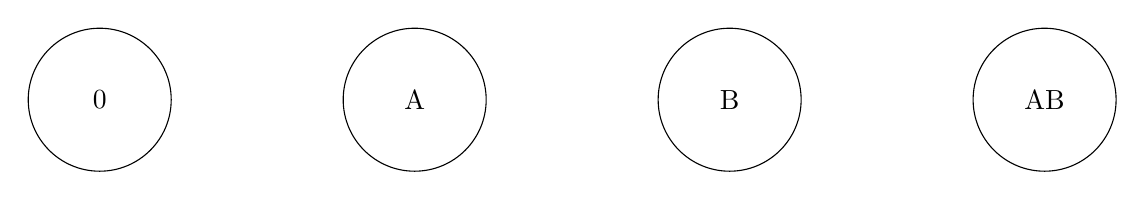
\begin{tikzpicture}[scale=1]
		\path[draw] (1,0) circle (6ex);\node at (1,0) {$0$};
		\path[draw] (5,0) circle (6ex);\node at (5,0) {A};
		\path[draw] (9,0) circle (6ex);\node at (9,0) {B};
		\path[draw] (13,0) circle (6ex);\node at (13,0) {AB};
	\end{tikzpicture}
	\vspace{2cm}
\end{minipage}



\vspace{0.4em}
\Kommentar{[Blutgruppen $A, B, AB, 0$ mit ihren Antigenen auf der Oberfläche]  }{}{0.8cm}{}

\vspace{0.3cm}
\enlargethispage{1.6cm}\hfill
\begin{minipage}[!h][][b]{12cm}
% % \setlength{\extrarowheight}{24pt} %% verträgt sich NICHT mit der Zentrierung
% \setcapmargin*[0cm]{0cm}
	\captionof{table}[Verzeichnis]{Punnet squar for the transfer of \textbf{blood} in the AB0-system \\ \textit{\textbf{remember:} There is NO "`universal donor"' for whole blood (serum \& cells) because when a transfer is done with whol blood, both antigens and antibodies must match! }}
	\begin{tabularx}{12cm}[]{m{2.2cm} | m{2.2cm} | m{2.2cm} | m{2.2cm} | m{2.2cm} m{0.1cm}  }% \toprule
	\textbf{Blut} & \centering \textbf{$0$} &\centering \textbf{A} &\centering \textbf{B} & \centering\textbf{AB}&   \\ [24pt] \midrule
	\textbf{$0$} &  & &  &  &  \\[24pt] \midrule
	\textbf{A}  &  & &  &   &  \\[24pt] \midrule
	\textbf{B} &  & &  & &  \\[24pt] \midrule
	\textbf{AB} &  & &  & &  \\[24pt] \midrule
	\end{tabularx}
\end{minipage}


%% I can't resume the list here - counter fails due to the dissection-counter (a workaround isn't trivial...)
% \ding{46} Copy the results from the blood typing test explained in \ding{229} Starr 34.7 (page 601) using the 8 circles below and write a short explanation about how this works!\label{exc:BloodTypeTheory}
%
%
% \vspace{0.6cm}
% 	\begin{tikzpicture}
% 		\path[draw] (1,0) circle (6ex);
% 		\path[draw] (5,0) circle (6ex);
% 		\path[draw] (10,0) circle (6ex);
% 		\path[draw] (14,0) circle (6ex);
% 	\end{tikzpicture}
% 	\vspace{0.3cm}
%
% 	\begin{tikzpicture}
% 		\path[draw] (1,0) circle (6ex);
% 		\path[draw] (5,0) circle (6ex);
% 		\path[draw] (10,0) circle (6ex);
% 		\path[draw] (14,0) circle (6ex);
% 	\end{tikzpicture}
%
% 	\vspace{2cm}
% \textbf{class activity:} Graphical explanation of antibodies and antigens:
% 		\vspace{1cm}
%
% 	\begin{tikzpicture}
% 		\path[draw] (1,0) circle (4ex);
% 		\path[draw] (5,0) circle (4ex);
% 		\path[draw] (10,0) circle (4ex);
% 		\path[draw] (14,0) circle (4ex);
% 	\end{tikzpicture}
%
% 	\vspace{2cm}



 \areaset[0cm]{14cm}{26.5cm}      
\subsubsection{Identify your own blood group and microsopy of red blood cells}
		\vspace{-0.6cm}
		\begin{center}
		 \fcolorbox{red}{Gray!20}{\parbox{14cm}{\centering
		\textbf{Taking a blood sample}     
		
		A drop of blood may transfer a sickness from one person to another! When working with blood, always do it the professional way!
		
		 \textit{Hint: in order to get your blood flowing \textbf{swing your arm} before pricking, in order to increase blood supply in your fingers.}
		}}
		\end{center}

		\marginpar{Until blood agglutination was understood most attempts to transfer blood between two persons failed. Since Landsteiner's discovery, Serum rich in antibodies can be used to test blood samples before donation: donor and recipient blood types must match!}

% \vspace{-0.6cm}
\paragraph{Materials:} Serum A; Serum B; Serum D; physiologische Kochsalzlösung (NaCl 0.9\%); 2 microscope slides tooth picks; blood lancets; swabs; disinfectant; paper towels; waist bin (jar with a plastic bag); cover slips; microscope
		\begin{enumerate}[label=\textit{(\arabic*)},leftmargin=1em,series=zaehler,itemsep=-2pt]
		      \item Get all your materials ready; mark the one microscope slide on the \textit{left} half with \textbf{A} and on the \textit{right} half with \textbf{B}; on the other slide you mark \textit{left} \textbf{D} and right \textbf{NaCl}

		      \item Use a swap and KODAN-disinfectant  in order to disinfect your finger.

		       \item Hold your hand against the table's surface and prick your finger with a \textsc{sterile} device and  \emph{immediately} press out those droplets!

		      \item You need four drops - two on each side of the two slides.

	              \item Trash the blood pricking tool. Use the your swap to sterilise your finger again, then trash the swab too.

		      \item Add one drop of \textbf{serum A }to the blood drop at the mark \emph{A}.
		      Add one drop of \textbf{serum B }to the blood drop at the mark \emph{B}.
		      Add one drop of \textbf{serum D }to the blood drop at the mark \emph{D}.
		      Add one drop of \textbf{NaCl 0.9\% }to the blood drop at the mark \emph{NaCl}.

		     \item Mix blood and serum - use a new tooth pick for each of the four tests (A, B, D, NaCl).

		     \item Can you observe \textbf{blood clumps}?  \gap{ yes: blood drop with serum A }
		      \item Compare your result with your sketches on page \pageref{exc:BloodTypeTheory}!
			      \begin{itemize}
			       \item your \texttt{A-B-0} blood group: \gap{\ldots A \ldots}
			       \item your D- or rhesus- blood group: \gap{\ldots D = Rh+ \ldots}
			      \end{itemize}
		      \item Trash your specimen (including the glass slides in the small bins!)
		\end{enumerate}
		
% \subsubsection{Red blood cells under the microscope}
% 		\begin{enumerate}[label=\textit{(\arabic*)},leftmargin=0em,series=zaehler]
% % 		      \item \sout{give a drop of blood onto a fresh slide}
% % 		      \item \sout{add a drop of 0.9\%  \ce{NaCl} }
% 		      \item observe one of your unclotted specimens from the AB0 test at 400x magnification
% 		      \item you may use Immersion oil and the 1000x mangification \textrightarrow~ clean the lenses afterwards!!
% 		      \item    if time allows: add a drop of strong salt solution (\textbf{ \ce{NaCl} 6\% }) to a specimen with unclotted blood and observe how osmosis produces misformed red blood cells
% 		\end{enumerate}
%

\vspace{0.5cm} \enlargethispage{1.6cm}
\Pointinghand\, Lets have a look at the "`universal donor"' of \textbf{blood cells} (table \ref{tab:Eryspende}) and the "`universal donor"' for \textbf{plasma} (table \ref{tab:Plasmaspende}):

\hspace{-2cm}
\begin{minipage}[!h][][b]{7.5cm}
	\captionof{table}[Verzeichnis]{Punnet squar for the transfer of \textbf{red blood cells} in the AB0-system } \label{tab:Eryspende}
	\begin{tabularx}{7.5cm}[]{m{1.4cm} | m{1.1cm} | m{1.1cm} | m{1.1cm} | m{1.1cm} m{0.1cm}  }% \toprule
	\textbf{Ery\-thro\-cyten} & \centering \textbf{$0$} &\centering \textbf{A} &\centering \textbf{B} & \centering\textbf{AB}&   \\ [6pt] \midrule
	\textbf{$0$} &  & &  &  &  \\[6pt] \midrule
	\textbf{A}  &  & &  &   &  \\[6pt] \midrule
	\textbf{B} &  & &  & &  \\[6pt] \midrule
	\textbf{AB} &  & &  & &  \\[6pt] \midrule
	\end{tabularx}
\end{minipage}
\hspace{1cm}
\begin{minipage}[!h][][b]{7.5cm}
	\captionof{table}[Verzeichnis]{Punnet squar for the transfer of \textbf{plasma} in the AB0-system} \label{tab:Plasmaspende}
	\begin{tabularx}{7.5cm}[]{m{1.4cm} | m{1.1cm} | m{1.1cm} | m{1.1cm} | m{1.1cm} m{0.1cm}  }% \toprule
	\textbf{Blut\-plasma} & \centering \textbf{$0$} &\centering \textbf{A} &\centering \textbf{B} & \centering\textbf{AB}&   \\ [6pt] \midrule
	\textbf{$0$} &  & &  &  &  \\[6pt] \midrule
	\textbf{A}  &  & &  &   &  \\[6pt] \midrule
	\textbf{B} &  & &  & &  \\[6pt] \midrule
	\textbf{AB} &  & &  & &  \\[6pt] \midrule
	\end{tabularx}
\end{minipage}


\begin{enumerate}[itemsep=1.5em, leftmargin=*]
\item  Why is every blood sample being divided into plasma and hematocrit?
	\Loesung{\\ In order help more patients with a single blood donation}{1cm}
\end{enumerate}

	 \areaset[0cm]{11.5cm}{27.4cm} %% (restore default)

	\cleardoublepage
%
% ... empty
% \clearpage

\section{Immunity}\label{sec:immunity}
% 	\marginnote{
% 		\begin{quotation}
% 		This section introduces to the battle of a complex organism, such as a human being, against small, agile and rapidly adapting invaders, such as bacteria, viruses, fungi and protozoans.
% 		\end{quotation}
% 			}

	\marginnote{\caution[t][BrickRed][what's about]{This topic is about complex organisms, such as a humans, on the one hand and small, agile, rapidly adapting invaders, such as bacteria, viruses, fungi or protozoans, on the other hand.}}[-0.6cm]


	 \marginnote{\caution[t][blue][films on moodle!]{A body with a healthy immune system eventually falls sick, but the absence of an immune system makes life unbearable: see \ding{253} \textsc{moodle} for film materials about our immune system.\\
	 \includegraphics[width=1.8cm]{/share/SB_Unterricht/moodle-QR-code.png}} }[3.5cm]


\begin{sloppypar}
  \begin{description}
\item \textsc{Topics of this chapter:}\\
You know what germs are and can give some examples\\
You understand the concept how our body distinguishes between self and non-self\\
You understand the function and anatomy of the lymphatic system\\
You can explain how the innate ("`non specific"') immunity fights off pathogens\\
You can explain how the adaptive ("`specific"') immunity fights off pathogens\\
You understand the concept of vaccination \\
You know some typical human diseases, including HIV-AIDS and Ebola\\
\end{description}
\end{sloppypar}


\subsection{Health, sickness}

\fboxp{12cm}{\textbf{Your personal definition of "`well being"' or \emph{health}:} \\
	\Kommentar{to me ``well being'' is to wake up in the morning and be able to take the coming day with ease, having plenty of energy }{}{1.6cm}{}
	}

\emph{"`disease"':}  \bgroup \color{DarkOrchid}  \bfseries  "`\textit{dis}"' = "`non"' and "`\textit{ease}"' = "`well-being"' \egroup

% \textbf{\emph{"`disease"':}}  \Answer{"`\textit{dis}"' = "`non"' and "`\textit{ease}"' = "`well-being"'}{0cm} \vspace{0.3cm}


What may cause a disease? Discuss this question with your group mate and take some notes about your findings:  \Answer{\fillwithdottedlines{2cm}}{2cm}
			\Loesung{\marginline{\href{/share/SB_Unterricht/Biology/hum11_immunobiology/Immune_ Biology_HS16.ppt}{link to ppt ``immunity''}}}{0cm}


\fboxp{14cm}{\textbf{Common terms related to diseases:} \\
	influenza (\textit{Grippe}), rubella (\textit{Röteln}), poliomyelitis (\textit{Kinderlähmung}), whooping cough (\textit{Keuchhusten}), stroke (\textit{Schlag (-anfall)}), anaemia (\textit{Blutarmut}), degenerative (\textit{abbauend}), anorexia (\textit{Magersucht}), obesity (\textit{Fettleibigkeit}), deficiency (\textit{Mangel}), Scurvy (\textit{Skorbut}), rickets (\textit{Rachitis}), essential (\textit{notwendig}), diphteria (\textit{Starrkrampf}), german measles (\textit{Wilde Blatern = Kuhpocken}), infectious disease (\textit{Infektionskrankheit}),
	epidemic (\textit{Infektionskrankheit}),
	pandemic  (\textit{Epidemie / Seuche }),
	malaria (\textit{Malaria}),
	plague (\textit{Pest}),
	cholera (\textit{Cholera}),
	World Health Organization (WHO) (\textit{Weltgesundheitsorganisation}),
	SARS (severe acute respiratory syndrome) (\textit{SARS}),
	droplet infection (\textit{Tröpfcheninfektion}),
	flu / influenza  (\textit{Grippe}),
	bird flue (\textit{Vogelgrippe}),
	swine flu (\textit{Schweinegrippe}),
	Health Impact Assessment (HIA) (\textit{Gesundheitsverträglichkeitsprüfung}),
	health prevention (\textit{Gesundheitsvorsorge}),
	Obama care (\textit{die vom US Präsidenten Obama eingeführte obligatorische Krankenversicherung}
	cow pox (\textit{Kuhpocken, ``Wilde Blatern''}),
	globalisation BE / globalization AE (\textit{Globalisierung}),
	travel advice (\textit{Reisetipp}),
	poverty (\textit{Armut}),
	developing country (\textit{Entwicklungsland}),
	newly industriaiised country (\textit{Schwellenland})
	}
\clearpage
\subsection{Pathogens - what we have to be prepared  for}
\subsubsection*{The six kingdoms of life}
\Pointinghand\, Study  \ding{229} Starr. fig. 1.6 (9ed) and note down the six kingdoms of life:
	\Kommentar{
			Archaea \\
			Bakteria \\
			Protista \\
			Fungi \\
			Plants \\
			Animals \\

			Kern / Zellwand / Grösse / Komplexität

			$\rightarrow\,$  Diskussion: welche Kriterien gewählt? Bekanntes / Unbekanntes? \\
			$\rightarrow\,$ Was ist mit den Viren? (... werden wir anschliessend anschauen)
			$\rightarrow\,$ Wer muss sich vor wem / was schützen?
						\vspace{2cm}
			}{}{6cm}{}

\subsubsection*{Bacteria}
\Pointinghand\, Structures of a bacterial cell

\textit{Literature:  \ding{229} Smith, p. 128 und \ding{229} Starr (9ed) Fig. 19.7}
	\Kommentar{


			$\rightarrow\,$  WT-Skizze entwickeln  \\
			$\rightarrow\,$ Wieso "'wollen"' Bakterien uns "'angreifen"`? \\
			$\rightarrow\,$ Was macht nun Bakterien für uns "'gefährlich"`?
			}{}{8cm}{}
\clearpage
\subsubsection*{Fungi}
\Pointinghand\, Structures of a fungal cell:

\textit{Literature:  \ding{229} Smith, p. 130 and \ding{229} Starr Fig. 22.6}

	\Kommentar{


			$\rightarrow\,$ Was unterscheidet Pilze von Bakterien? \\
			$\rightarrow\,$  WT-Skizze entwickeln  \\
			$\rightarrow\,$ Wieso leiden wir selten an "'Verpilzung"`?
			}{}{8cm}{}


\subsubsection*{Viruses}
\Pointinghand\, Structures of a virus:

	\textit{Literature: \ding{229} Smith, S. 129 and \ding{229} Starr 19.4}
	\vfill

 \areaset[0cm]{11.5cm}{27.4cm}


\subsubsection{Visualisation of the first line of defence}
			\piccaptionside
		%\setcapmargin*[-2cm ]{0cm }
		\piccaption[VERWEIS]{\label{fig:LABEL}
		visualisation of the \emph{first line of defence} in human body: \\[6pt]
		a) mechanical barrier and chemical protection (acids in sweat and sebum (\textit{Talg}))\\[6pt]
		b) good bacteria competing against pathogenic bacteria\\[6pt]
		c) cilia (\textit{Flimmerhäärchen})\\[6pt]
		d) lysozym and other enzymes\\[6pt]
		e) flush off by urine\\[6pt]
		f) acids \\[6pt]
		g) acid milieu produced by mucous membranes (\textit{Schleimhäute})\\[6pt]
		h) saliva and mucous (with lysozym), sneezing and coughing
		}
		\parpic[l]{\includegraphics[width=6cm]{/share/SB_Unterricht/Biologie/hum11_Immunbiologie/Immunbio-Lieske_HS12/Immun-ppt-noraHS12-033.png}}
%		\picskip{0}
		%\setcapmargin*[0cm ]{0cm }



\vspace{2cm}
\subsection{Hygiene - not to be underestimated}
		\marginline{\Loesung{\href{/share/SB_Unterricht/Biology/hum11_immunobiology/SurgicalCabinet-1870s_Nufield01_v2.png}{Hygiene was once highly critically neglected: Surgical Cabinet in 1870}}{0cm}}
Most people will connect microbes with disease, although many microbes are beneficial and useful to man and many more are quite harmless. Disease-causing microbes are, in fact, normally in the minority. Microorganisms are widespread and quickly multiply, therefore a small number of harmful germs may quickly develop a large community. It is obviously desirable to control the spread of those microbes which cause food to spoil and those which cause infection and disease.

You can test the effect of washing your hands: First, dig one finger into fresh soil, gently rub the dirt off and place this finger onto Petri dish \# 1. Second, thoroughly wash your hands with soap, blot them dry with a \emph{clean} towel and place one finger onto Petri Dish \# 2. Use one petri dish for up to four persons. Your plates will be incubated at for 2 days at 37\degreecelsius. Next week you will record the results:

		\todol{get Petri dishes ready!}

	\begin{tikzpicture}
		\path[draw] (1,0) circle (16ex);
		\path[draw] (9,0) circle (16ex);
	\end{tikzpicture}

		% % % an interesting on the immunity of the airways:

			% \commentpage{false}{
			% 	\subsection*{Defence of the airways}
			% 	(from: \url{http://www.merckmanuals.com/home/lung-and-airway-disorders/biology-of-the-lungs-and-airways/defense-mechanisms-of-the-respiratory-system}
			%
			% 		The average person who is moderately active during the daytime breathes about 20,000 liters (more than 5,000 gallons) of air every 24 hours. Inevitably, this air (which would weigh more than 20 kilograms [44 pounds]) contains potentially harmful particles and gases. Particles, such as dust and soot, mold, fungi, bacteria, and viruses deposit on airway and alveolar surfaces. Fortunately, the respiratory system has defense mechanisms to clean and protect itself. Only extremely small particles, less than 3 to 5 microns (0.000118 to 0.000196 inches) in diameter, penetrate to the deep lung.
			%
			% 		One of the respiratory system's defense mechanisms involves tiny, muscular, hair-like projections (cilia) on the cells that line the airways. The airways are covered by a liquid layer of mucus that is propelled by the cilia. These tiny muscles beat more than 1,000 times a minute, moving the mucus that lines the trachea upwards about 0.5 to 1 centimeter per minute (0.197 to 0.4 inch per minute). Particles and pathogens that are trapped on this mucus layer are coughed out or moved to the mouth and swallowed.
			%
			% 		Because of the requirements of gas exchange, alveoli are not protected by mucus and cilia—mucus is too thick and would slow movement of oxygen and carbon dioxide. Instead, the body has another defense system. Mobile cells on the alveolar surface called phagocytes seek out deposited particles, bind to them, ingest them, kill any that are living, and digest them. The phagocytes in alveoli of the lungs are called alveolar macrophages. When the lungs are exposed to serious threats, additional white blood cells in the circulation, especially neutrophils, can be recruited to help ingest and kill pathogens (foreign particles). For example, when the person inhales a great deal of dust or is fighting a respiratory infection, more macrophages are produced and neutrophils are recruited.
			% 	}
			% %*******************************************



\clearpage
\subsection{The lymphatic system}\label{ssc:LymphSystem}

			\begin{mdframed}[style=exampledefault, userdefinedwidth=12cm,frametitle={Starr chapter 33.10}\label{mat:BEISPIELMATERIAL}]
			The \emph{lymphatic system} connects the circulatory system to the immune system: read about this system of small vessels and clumps of pathogen fighting cells \ding{229} p. 584.
		\end{mdframed}

	\begin{enumerate}[leftmargin=*]
	\item Use figure \ref{fig:LymphSystOverv} to test your knowledge: annotate it with a legend and write short definitions for the lymphatic organs shown in this figure!
	\end{enumerate}

			\marginnote{\caution[c][blue][film!]{Find an animated illustration of the lymphatic system on \ding{253} \textsc{moodle}
% 			 \href{https://cloudfs.tam.ch/share?t=5897f135a641e69b178b464a5897f197d341a2.87745049}{\ding{253}kzucloud}
			}}


	\vspace{4pt}
	 \Ersatz{
	\begin{minipage}[htbp]{12cm}
	\includegraphics[width=10cm]{/images/biozone-human-0137-1_v1.png}\captionof{figure}[lymph syst from biozone humanbiol p. 137]{The lymphatic system: label the figure according to figure 33.21 (Starr 9ed) in your textbook}  	\label{fig:LymphSystOverv}
	\end{minipage}
	}{%%
	\begin{minipage}[htbp]{12cm}
	\includegraphics[width=10cm]{/images/biozone-human-0137-1_v2.png}\captionof{figure}[lymph syst from biozone humanbiol p. 137]{The lymphatic system: label the figure according to figure 33.21 (Starr 9ed)}  	\label{fig:LymphSystOverv}
	\end{minipage}
	}



\clearpage
\subsection{Three lines of defence}\label{sec:ThreeLinesDefence}
				\begin{mdframed}[style=exampledefault, userdefinedwidth=12cm,frametitle={Starr chapter 34.1}\label{mat:BEISPIELMATERIAL}]
			Our body is warm, wet and full of delicious nutrients - a feast for every microorganism!
			Under the title \textit{What is immunity} you can find a conceptual introduction to the way our body fights off pathogens.
		\end{mdframed}

%  We learned from human history different solutions in this situation: you either fully protect your wealth - you will have to start an arms race (\textit{"'Wettrüsten"', see the cold war}) or rule and divide (\textit{"`herrsche und teile"`, as during the colonial time}). You never can be sure to protect your goods and eventually you get sick and finally you will die, getting rotten by microorganisms.



The arms race against "`bad"' microorganisms is lined up in three lines of defence:

	\begin{enumerate}[itemsep=1.5em, leftmargin=*]
	\item   Match the following terms with the corresponding line of defence:  \textsc{
	adaptive immunity; mechanical barrier; innate immunity; phagocytic white blood cells; lymphocytes, cellular response, chemical barrier; inflammatory response; secretion of mucus; antibodies; antimicrobial proteins; skin; complement proteins}.

	\item Explain which of these three lines are \textbf{unspecific}, which are \textbf{specific} against \textsc{certain germs}!
	\end{enumerate}
%
				\Loesung{\marginline{\href{/share/SB_Unterricht/Biology/hum11_immunobiology/Immune_ Biology_HS16.ppt}{link to ppt ``immunity''}}}{0cm}

% % 	\begin{addmargin*}[-.5cm]{-1.5cm}
	\hspace{-3.6cm}
	 \begin{minipage}{16cm}
		\setlength{\extrarowheight}{6pt}
		 \captionof{table}{Characteristics of the three lines of defence}
		  \vspace{12pt}
		    \begin{tabularx}{16cm}[]{p{5cm} p{5cm} p{6cm}} %
		\toprule
		First line of defence & Second line of defence  & Third line of defence \\\midrule
		 \gap{mechanical barrier}   &  \gap{phagoc. white blood cells} &  \gap{adaptive immunity}\\
		 \gap{chemical barrier}   & \gap{inflammatory response}  & \gap{lymphocytes} \\
		 \gap{secretion of mucus}   &  \gap{complement proteins} & \gap{cellular response} \\
		 \gap{skin}   & \gap{innate immunity}  & \gap{antibodies} \\
		 \gap{antimicrobial proteins} &  &  \\
		\bottomrule
		\end{tabularx}%
		  \label{tab:ThreeLinesDefence}%
	\end{minipage}
% % 	\end{addmargin*}


% \Ersatz{\vspace{0cm}\enlargethispage{2cm} }{\vspace{1cm}}
% \Ersatz{\hspace{-1cm}}{\hspace{-1cm}}

	\vspace{1cm}
	\begin{enumerate}[resume,itemsep=4pt, leftmargin=0cm]
	\item  Use \ding{229} Starr chapter 34 to assist you filling in the cross word (\autoref{fig:CrissCrossBodyDefense})
	\end{enumerate}

	\enlargethispage{2cm}
	\hspace{-3.6cm}
	\begin{minipage}{16cm}
			\begin{multicols}{2}
			\bgroup \Ersatz{\tiny}{\small}
			1. an organism's capacity to resist and combat an infection
				\Loesung{\\ immunity}{0cm}

			2. which underlying process developed the concept of self and non-self?
				\Loesung{\\ evolution}{0cm}

			3. abbreviation for non-self cues
				\Loesung{\\ pamp}{0cm}

			4. set of proteins that can destroy invading cells
				\Loesung{\\ complement}{0cm}

			5. a fast general defence against infection
				\Loesung{\\ innate immunity}{0cm}

			6. what stands the abbreviation 'PAMP' for?
				\Loesung{\\ pathogen associated molecular patterns}{0cm}

			7. a tailored immune defense
				\Loesung{\\ adaptive immunity}{0cm}

			8. cells that mount a quick secondary response even years after a first infection with a specific antigen
				\Loesung{\\ memory cells}{0cm}

			9. physical, chemical and mechanical barriers against invaders are called the [...] of defense
				\Loesung{\\ first line)}{0cm}

			10. a cell that moves around and engulfs ('eats') other cells is ...
				\Loesung{\\ phagocytic}{0cm}

			11. general term for substances which allow partners of the immune system to communicate
				\Loesung{\\ cytokines}{0cm}

			12. The most abundant phagocytic cells are
				\Loesung{\\ neutrophiles}{0cm}

			13. interleukins and interferons are
				\Loesung{\\ cytokines}{0cm}

			14. Cells of the innate immune system which alert the adaptive immune system
				\Loesung{\\ cendritic cells}{0cm}

			15. Eosinophiles contain vesicles filled with destructive enzymes targeting
				\Loesung{\\ parasites}{0cm}

			16. The nervous system may cause degranulation of
				\Loesung{\\ mast cells}{0cm}

			17. Cell of the adaptive immune system, recognizing a specific antigen:
				\Loesung{\\ lymphocyte}{0cm}

			18. an infected cell may be destroyed by a
				\Loesung{\\ cytotoxic t-cell}{0cm}

			19. a cancerous (von Krebs befallen) cell may be destroyed by a
				\Loesung{\\ natural killer cell}{0cm}

			20. approximative number of different antigens detected by the innate immune system
				\Loesung{\\ thousand}{0cm}

			21. approx. response time for the adaptive immune system - in 'days'
				\Loesung{\\ seven}{0cm}
			 \egroup
	\end{multicols}
	\end{minipage}

%
% 	\vspace{4pt}
% 	\hspace{1cm}
	 \areaset[0cm]{20cm}{28cm}
	\thispagestyle{empty}
	\Ersatz{
		\begin{minipage}[htbp]{22cm}
		\centering {\includegraphics[width=1\textwidth,angle=90]{/share/SB_Unterricht/Biology/hum11_immunobiology/BodyDefence-CrissCross_L_v2.png}} \captionof{figure}[VERZEICHNISEINTRAG]{Crossword on immune response - introduction}  	\label{fig:CrissCrossBodyDefense}
		\vspace{2pt}
		\end{minipage}
		}%
		{
		\begin{minipage}[htbp]{20cm}
		\centering {\includegraphics[width=1\textwidth]{/share/SB_Unterricht/Biology/hum11_immunobiology/BodyDefence-CrissCross_S_v3}} \captionof{figure}[VERZEICHNISEINTRAG]{Crossword on immune response - introduction}  	\label{fig:CrissCrossBodyDefense}
		\vspace{2pt}
		\end{minipage}
		}%


 \areaset[0cm]{15cm}{27.4cm}
\subsection{How cells recognise each another and form tissues}
\Pointinghand\, May cells erronously stick to the wrong partner? The following figures  (\textit{taken vorm Markl, chp 3.2}) give you an answer:

\begin{enumerate}[itemsep=1.5em, leftmargin=*]
\item  The cells of two differently colored sponges (\textit{yes, these are living organisms!}) of the same species were isolated through a sieve and then mixed up. Describe the outcome of this experiment and draw a general conclusion!
\end{enumerate}
			\vspace{1.4cm}
			\begin{figure}[htp]\centering
		  \includegraphics[width=0.5\textwidth]{/share/00_SCHULE_DATA-add/bilder_saz/Markl_Bilder/1_4_Zellen/3_Biomembranen_und_Transportvorgaenge/03_02_01_1.jpg}
		  \caption[Schwammzellen finden sich aus Markl 3.2]{Cells of two different sponges were experimentally mixed (coloured figure in Markl 3.2 or on \ding{253} \textsc{Moodle}).}
		  \label{fig:SchwammZellen}
		%\setfloatalignment{b}
		\end{figure}

			\begin{figure}[htp] \centering
		  \includegraphics[width=0.5\textwidth]{/share/00_SCHULE_DATA-add/bilder_saz/Markl_Bilder/1_4_Zellen/3_Biomembranen_und_Transportvorgaenge/03_01_01_1_v1.jpg}
		  \caption[Aufbau Zellmembran aus Markl 3.1]{Fluid mosaic model of cell membranes (coloured figure in Starr (9ed) 4.3 or on \ding{253} \textsc{Moodle})}
		  \label{fig:ZellmembraneGlykolipide}
		%\setfloatalignment{b}
		\end{figure}

\clearpage
\subsection{The family tree of blood cells}
\Pointinghand\, Knowing the "`who is who"' in the family of blood cells tells us what they may have in common and how they are related to each other:

\hspace{-3cm}
    \begin{figure}[htbp]
    \begin{minipage}{7cm}

      \includegraphics[width=0.8\textwidth]{/share/00_SCHULE_DATA-add/bilder_saz/Markl_Bilder/9_16_Genetik/13_Entwicklungsgenetik/13_04_01_0.jpg}
      \caption{The various blood cells stem from multi-potent stem cells. (\textit{figure taken from Markl, 13.4}) }  \label{fig:BlutGenese}
    \end{minipage}\hfill
    \begin{minipage}{9cm}
     \hfill
      \includegraphics[width=0.8\textwidth]{/share/00_SCHULE_DATA-add/bilder_saz/Humanbio_Bilder/Anatomie_MalAtlas_en/AnatomyCol-121_v1.png}
      \caption{White blood cells need to be trained for their job (\textit{from Markl Kap. 16.1.}) \textbf{A} Bone Marrow; \textbf{T} Thymus; \textbf{C} Spleen; \textbf{D} Lymph node; \textbf{E} lymphatic tissue connected to the intestines; \textbf{F} Tonsils; \textbf{G} Appendix; \textbf{B} B-Lymphocytes; \textbf{PC} Plasma-Cell; \textbf{TH} T-Helper-Cell; \textbf{TC} T-Cytotoxic-Cell; \textbf{NK} Natural Killer Cell; \textbf{P} Phagocyte
      }  \label{fig:LymphOrgane}
    \end{minipage}
	 \end{figure}



\Lehrer{ \vspace{2cm}
		Diskussion des Konzepts Stammzelle\\
		Einführen der Typen von weissen B.K.\\
		Bildungs- und Ausbildungs-Orte der weissen B.K.
		}

\clearpage \enlargethispage{1.8cm}
\subsection{Discrimination of self and foreign}
\Pointinghand\, This chapter explains how our immune system discriminates self from foreign - a prerequisite to any action against pathogens.

\subsubsection{The Major Histocompatibility Complex One (MHC-I) acts as the cells' identity card}
\begin{mdframed}[style=RedGray]
\textbf{ 1.} NO infection present: "`safe"' and healthy every day life of cell.
\end{mdframed}


% \begin{mdframed}[style=RedGray]
	\begin{minipage}{14cm}
	 \centering
		\includegraphics[width=1\textwidth]{/share/00_SCHULE_DATA-add/bilder_saz/Humanbio_Bilder/humanbio_Tortora-en/ch22/pap14_fig_22_14.jpg}
	\end{minipage}
% 	\end{mdframed}
\vspace{2cm}

%
% 	\setlength{\extrarowheight}{4pt}
% 	\begin{tabularx}{14cm}[]{>{\textbf}m{0.7cm} >{\textsc}m{3cm} X} \toprule
% 	\textbf{Nr} &  \textbf{Prozess} \\ \midrule
% 	1 &  Lysosom  & Abbau von zelleigenen Proteinen in Peptidfragmente \\
% 	2 & Endopl. Retic. (ER) & Synthese von MHC Molekülen in ein Vesikel  \\
% 	3 & Golgi-Vesikel & Vesikel mit MHC-I nimmt Peptid (Proteinbruchstücke) auf und wird zum MHC-Vesikel \\
% 	4 & MHC-Vesikel &  Peptide werden an MHC-I gebunden und wandert zur Zellmembran \\
% 	5 & Zellmembran & Exocytose des mit Peptid beladenen MHC-I Komplexes und Einbau in die Zellmembran \\
% 	6 & Zellmembran & tausende von MHC-I Komplexe über der ganzen Zelloberfläche zeigen laufend die typischen zelleigenen Proteine \\
% 	\bottomrule
% \end{tabularx}

\vfill \bgroup \centering
\Pointinghand\, The cells of the immune system permanently scan the surface of every body cell. As long as the immune system encounters well known protein-fragments posted on MHC-I the cell is considered healthy and the immune system won't get activated. \egroup
\vfill

\clearpage
\subsubsection{In case of an infection, MHC-I triggers the "`alarm"'}
\vspace{0.2cm}
\begin{mdframed}[style=RedGray] \textbf{2.} An infection (or a tumor) is present: this means "`sickness"' to any kind of cells. \end{mdframed}

% \Kommentar{
% \begin{mdframed}[style=RedGray]
	\begin{minipage}{16cm}
	 \centering \vspace{0.4cm}
		\includegraphics[width=0.7\textwidth]{/share/00_SCHULE_DATA-add/bilder_saz/Humanbio_Bilder/humanbio_Tortora-en/ch22/pap14_fig_22_14.jpg}
	\end{minipage}
	% 	\end{mdframed}
	\vspace{0.2cm} This is the \textsc{same} figure as on the previous page \textsc{but} DIFFERENT proteins are shown: fragments of either a \textbf{virus} or distorted proteins e.g. typical for \textbf{cancer}.
% 		}{}{5cm}{}

\vspace{0.3cm}
\bgroup \centering \Pointinghand\, Whenever a cell presents unusual proteins such as virus fragments or proteins that derive from a mutation within the cell's genome on its MHC-1 flag poles the immune system sets the alarm! This starts the immune response to fight off every cell that shows the same type of antigen (\textit{"`strange or foreign protein"'})!
\egroup

\enlargethispage{1.4cm}
\vfill
	\hfill	\begin{mdframed}[style=exampledefault,leftmargin=-1cm, userdefinedwidth=16cm,frametitle={\hfill Antigene: "`antibody generating agent"'\hfill}\label{mat:BEISPIELMATERIAL}]
			Every structure which causes the formation of antibodies is called an \textsc{antigen}. Examples are the surface proteins of erythrocytes (see the \textsc{AB0}-blood-system) OR strange proteinfragments shown on MHC-1 (\textit{this chapter}) OR surface structures of pathogens (see fig.\ref{fig:AntigeneEpitopeAntikoerper}) OR surface structures various kind of foreign matter such as pollen (hay fever).\\
			\emph{note} the difference between  \emph{antigen} and \emph{epitop} as shown here:

	 \centering
		  \includegraphics[width=0.5\textwidth]{/share/00_SCHULE_DATA-add/bilder_saz/Purves/abbildungen/kap-18/18-06_v2.jpg}
		  \captionof{figure}[Antigene, Epitope, Antikörper; aus Purves, 7. Aufl. 2006, Abb. 18-06]{An \textbf{epitop} is a specific part of an antigen which causes the formation of a specific antibody (see  \ding{229} Starr ... }
		  \label{fig:AntigeneEpitopeAntikoerper}
		\end{mdframed}
% \vspace{1cm}

\clearpage
\subsection{Phagocytosis, cells of the immune system and MHC-II}
\Pointinghand\, Cells of the immune system are capable of \textsc{phagocytisis}, i.e. to ingest and digest foreign cells and other particles. Fragments of the eaten up foreign material is presented attached to "`Major Histocompatibility Complexes Two"` (MHC-II) on the outer membrane of \textsc{antigen presenting cells}:

\vspace{1cm}
% \Kommentar{
% \begin{mdframed}[style=RedGray]
	\begin{minipage}{12cm}
	 \centering
		\includegraphics[width=1\textwidth]{/share/00_SCHULE_DATA-add/bilder_saz/Humanbio_Bilder/humanbio_Tortora-en/ch22/pap14_fig_22_13.jpg}
	\end{minipage}
% 	\end{mdframed} \vspace{0.2cm}
% 		}{}{6cm}{}

% 	\setlength{\extrarowheight}{4pt}
% 	\begin{tabularx}{14cm}[]{>{\textbf}m{0.7cm} >{\textsc}m{3cm} X} \toprule
% 	\textbf{Nr} &  \textbf{Prozess} \\ \midrule
% 	1 & Zellmembran & Phagocytose (\textit{Zellfressen}) eines Antigens \\
% 	2 & Phagosom (Vesikel) & Verdau des Antigens in Peptidfragmente \\
% 	3 & Endopl. Retic. (ER) & Synthese von MHC Molekülen und Verpackung in ein Vesikel  \\
% 	4 & Vesikel & Verschmelzung von  Phagosom und MHC-Vesikel  \\
% 	5 & MHC-Vesikel & Antigen-Peptidfragmente binden an MHC-II Moleküle \\
% 	6 & Zellmembrane & Die MHC-II Komplexe zeigen die fremden Proteine (Peptid-Fragmente) auf der Zelloberfläche. Das ist eine Alarmglocke! \\
% 	\bottomrule
% \end{tabularx}


\vfill
		\begin{mdframed}[style=exampledefault,leftmargin=2cm userdefinedwidth=14cm,frametitle={MHC-I, MHC-II and Interleukins allow to trigger a immune reaction }\label{mat:BEISPIELMATERIAL}]
			Aberrant material (antigens) presented both on MHC-I and / or MHC-II triggers the communication among cells of the immune system. In response the cells of the immune system produce signalling chemicals, referred to \textsc{cytokines} or more specific to \textsc{interleukins}

			\centering Communication among cells is crucial at the interface of \textsc{unspecific} and \textsc{specific} immune response as well as in the coordination and control of the highly complex specific immune response.
		\end{mdframed}
	\vspace{1cm}



\clearpage \enlargethispage{1.6cm}
\subsection{Antibodies and Receptors}
\Pointinghand\,\, Both secreted antibodies \emph{freely moving in blood and lymph} and receptors \emph{membrane bound antibodies} are the counter players of antigens - they do recognise them. You already well know the antibodies of the $AB0$-blood group system, that match the respective antigens. Lets now have a closer look:


		\begin{minipage}{9cm}
		  \includegraphics[width=0.9\textwidth]{/share/SB_Unterricht/Biologie/hum11_Immunbiologie/Antikoerper-Rezeptor_Kuby-Fig-01-07_v2.jpg}
		  \captionof{figure}[B-Rezeptor und B Antikörper aus Kuby 8th ed. p. 12 (Fig. 1-7)]{Model of a free moving (secreted) antibody (left) and a receptor attached to the membrane (right)  \textit{source: Kuby, 8th ed.} More details in  \ding{229} Starr (9ed) 34.4 }
		  \label{fig:RezeptorAntikoerper}
		\end{minipage}
% 		\hspace{0.4cm}
		\begin{minipage}{6cm}
		 \includegraphics[width=1\textwidth]{/share/SB_Unterricht/Biologie/hum11_Immunbiologie/Toll-Rezeptor_Kuby-Fig-03-010_v2.jpg}
		  \captionof{figure}[Toll-Rezeptor aus Kuby 8th ed p. 63 (Fig. 3-10)]{Toll receptor of a macrophage - this receptor matches with typical glykolipids (or glykoproteins) on the surface of bacteria \textit{Quelle: Kuby, 8th ed.}}
		  \label{fig:TollRezptor}
		\end{minipage}

		\begin{mdframed}[style=exampledefault, userdefinedwidth=16cm,frametitle={Toll-receptors, Immunoglobulines, cell-bound Receptors }\label{mat:BEISPIELMATERIAL}]
			\begin{itemize}
				\item Toll Receptors are found on the surface of macrophages and they are crucial in the \textsc{innate} immune response.

				\item Toll receptors recognise typical surface antigens ($\rightarrow$~ "' \textit{unspecific response"`}) of most bacteria and allow macrophages to immediately phagocyte the bacteria.

				\item Immunoglobulines (Ig) are the typical kind of secreted antibodies and they are crucial in the \textsc{adaptive immune response}.

				\item Membrane-bound receptors of the \textsc{lymphocytes} recognise antigens attached to either  MHC-I or MHC-II.

				\item Every type of immunglobuline (Ig) or membrane-bound-receptor can identify a single type of antigen.

				\item Because their are billions of different antibodies (Ig or receptors) one will always match to a new kind of antigen!
			\end{itemize}
		\end{mdframed}





		\begin{minipage}{15.5cm}\centering
		  \includegraphics[width=0.9\textwidth]{/share/SB_Unterricht/Biologie/hum11_Immunbiologie/Ecoli-Lipopolysaccharide_Kuby-Fig-03-09_v1.png}
		  \captionof{figure}[E. coli Zellwand aus Kuby 8th ed p. 63 (Fig. 3-9)]{Darstellung der Zellwand eines \textit{E. coli} (Darm-)Bakteriums: Die Lipopolysaccharide auf der Aussenseite werden (in der Regel) von den Toll-Rezeptoren der Makrophagen erkannt und lösen die \textsc{unspezifische} Immunreaktion aus. \textit{Quelle: Kuby, 8th ed.}}
		  \label{fig:BakterienZellwand}
		\end{minipage}

% \areaset[0cm]{11.5cm}{27.4cm}
\subsection{Innate immunity - your second line of defence}\label{sec:ImmuneInnate}\label{ssc:ImmuneInnate}
Work with your textbook \ding{229} chapter 34.4 (Starr 9ed 34.3).

		\begin{mdframed}[style=exampledefault, userdefinedwidth=12cm,frametitle={Starr chapter 34.3}\label{mat:BEISPIELMATERIAL}]
			Starr explains you which types of cells are capable of phagocytosis. The \emph{complement}-proteins form another part of the innate immune system. The \emph{inflammation} is the ``battle field'' of the innate immune system and \emph{fever} is the recordable outcome of such a kind of immune reaction.
		\end{mdframed}

	\begin{enumerate}[itemsep=1.5em, resume, leftmargin=*]
	\item  Match the terms and explanations in table \ref{tab:InnateImmunityLabels} with the charts in figure \ref{fig:InnateImmunityFigure}!
	\end{enumerate}

% 			\begin{figure}[htp]
				\begin{addmargin*}[-2cm]{-2cm}
	 \begin{minipage}{16cm}
		  \includegraphics[width=1\textwidth]{/images/biozone-human-0135_v3.png}
		  \captionof{figure}[VERZEICHNISEINTRAG]{The innate immune reaction, synopsis}
		  \label{fig:InnateImmunityFigure}
		%\setfloatalignment{b}
% 		\end{figure}
	 \end{minipage}
				\end{addmargin*}


	\begin{addmargin*}[-2cm]{-2cm}
	 \begin{minipage}{16cm}
% 		 \begin{table}[!htbp]
		\setlength{\extrarowheight}{6pt}
		 \captionof{table}{Text pieces taken from figure \ref{fig:InnateImmunityFigure}}
		  \vspace{12pt}
		    \begin{tabularx}{16cm}[]{X p{2cm}} %
		\toprule
		Structure or function& Legend for figure \ref{fig:InnateImmunityFigure}   \\\midrule
		Bacteria are engulfed and destroyed by phagccytes (macrophages and neutrophils).  & \gap{  6 } \\
		Bacteria entering on knife or other sharp object.   & \gap{  2 } \\
		 Phagocytes stick to capillary walls.  & \gap{ 9  } \\
		 Bacterium  & \gap{  1 } \\
		Blood vessels increase diameter (vasodilatation) and permeability.  & \gap{ 4  } \\
		Capillary wall & \gap{  7 } \\
		Red blood cells & \gap{8   } \\
		Phagocytes squeeze between cells making up blood vessel walls.   & \gap{ 5  } \\
		Chemicals (e.g. histamines and prostaglandins) are released by damaged cells, attracting more and more phagocytes to this infection.   & \gap{ 3  } \\
		\bottomrule
		\end{tabularx}%
		  \label{tab:ThreeLinesDefence}%
% 		\end{table}%
	\end{minipage}
	\end{addmargin*}


\subsubsection{Opsonierung von Krankheitserregern}
\Pointinghand\, Der Wirbeltierkörper produziert Proteine ("'Opsonine"`), welche auf der Oberfläche von Bakterienzellwänden an Oberflächenstrukturen haften, welche es bei vielen Bakterien, aber nicht bei tierischen Zellen gibt. Diese Opsonine wirken für die Fresszellen wie Signalfahnen: "'\textit{Achtung, hierhin und auffressen!}"`. \Forward\, \href{https://cloudfs.tam.ch/share/b57cd0560b90e9f2b2f344aaef286649}{Animationsfilm zur Opsonierung auf  \ding{229} moodle }

\subsubsection{Das Komplementsystem}
\Pointinghand\, Wie bei den Opsoninen, binden die Komplementproteine and Bakterienoberflächen  \ding{229} Markl Kap. 16.2 (ganz am Schluss) und \href{https://cloudfs.tam.ch/share/362f92164b2771f7806ebc86e1db186b}{Animation zum Komplementsystem}


\subsubsection{Fieber unterstützt die Abwehrreaktion}

\begin{enumerate}[itemsep=1.5em, leftmargin=*]
\item  Lesen Sie den nachfolgenden Text übers Fieber - wo nötig setzen Sie ihren Dictionnaire ein! Machen Sie sich passende (Rand-)Notizen!
\end{enumerate}

\begin{minipage}{16cm}
	\includegraphics[width=1\textwidth]{/images/biozone-human-0136_v2.jpg}
	 \captionof{figure}[Fieberdarstellung aus Biozone Humans p.136]{Eine erhöhte Körpertemperatur unterstützt die Heilung effizient, denn das Wachstum vieler Bakterien wird gehemmt und metabolische Prozesse laufen rascher ab (Teilchenbewegung, RGT-Regel). Die normale Körpertemperatur liegt bei 36.2 bis 37.2\degreecelsius\, und Temperaturen über 45.5\degreecelsius\, bedeutet Todesgefahr.}
\end{minipage}



\clearpage
\subsection{Adaptive Immune Response (third line of defence)}\label{ssc:AdaptiveImmunity}

		\begin{mdframed}[style=exampledefault, userdefinedwidth=12cm,frametitle={Starr chapter 34.4}\label{mat:BEISPIELMATERIAL}]
			Not the editor's choice this spread, but fine to make you acquainted with the sheer infinite variability of receptors, antigens and antibodies. Read this section carefully and make sure you understand the concepts. However, don't learn by heart the five classes of antibodies (\ding{229} Table 34.3).
		\end{mdframed}

	\begin{enumerate}[resume, leftmargin=*]
	\item  Explain in your words how \textit{antigen diversity arises} (\ding{229}, Fig. 34.9)
		\Loesung{ \vspace{3cm}} {3cm}
	\end{enumerate}

		\hspace{-2cm}
		\begin{minipage}{18cm}
		  \includegraphics[width=1\textwidth]{/share/00_SCHULE_DATA-add/bilder_saz/Humanbio_Bilder/physiolo-coloringbook/PhysiolColor_148_v1.png}
		  \captionof{figure}[Physiology Coloring Book p. 148 v1, Ineterleukins]{How interleukins (IL) coordinate the processes of the adaptive immune response}
		  \label{fig:Interleukins}
		\end{minipage}

		\begin{mdframed}[style=exampledefault, userdefinedwidth=12cm,frametitle={Starr, chapter 34.5}\label{mat:BEISPIELMATERIAL}]
			Here, Starr introduces you to the concept of \emph{adaptive immunity} on an easy level
		\end{mdframed}
\vfill
				\begin{mdframed}[style=exampledefault, userdefinedwidth=12cm,frametitle={Starr chapters 24.6 and 34.8}\label{mat:BEISPIELMATERIAL}]
			These two (sub-) chapters explain the details of both antibody-mediated (= ``humoral``) immune response (\ding{229} 34.6) and cell-mediated immune response (\ding{229}  34.8). As a piece of advice you should use figure \ref{fig:ImmuneAdaptiveEvaHo} on page \pageref{fig:ImmuneAdaptiveEvaHo} as a scaffold (\textit{a frame}).
		\end{mdframed}

		\marginnote{\caution[c][blue][film!]{\ding{253} Find a selection of youtube movies on \textsc{moodle} that may help you for a better understanding of these complicated processes.
		}}


\begin{enumerate}[resume, leftmargin=*]

% \item The charts A through D in figure \ref{fig:ImmuneAdaptiveTortora} shows you several aspects of the adaptive immune response in greater detail. Carefully study these charts in order to understand the functions (and duties) of all the cells and molecules involved!

\item Figure \ref{fig:ImmuneAdaptiveEvaHo} summarises the \textsc{Adaptive Immune Response}. Use the \textsc{Compad} materials to visualise this scheme AND produce a \textsc{stop-motion film} or a series of \textsc{power point }slides.

% \item In order to revise the entire topic of immune response you'll be provided with a card game - just ask your teacher about.

\end{enumerate}
\vfill
\clearpage
			% %% may be provided as coloured copies   %%%%%%%%%%%%%%%
			% \clearpage  \thispagestyle{empty}
			% 		\begin{minipage}{16cm}
			% 		\hspace{-2cm}
			% 			\includegraphics[width=1\textwidth]{/share/SB_Unterricht/Biology/hum11_immunobiology/immune-adaptive/AdaptiveImmunity_picts-Tortora_HS16_v1.pdf}
			% 			\captionof{figure}[Adaptive Immune System charts from Tortora ch. 22]{Adaptive Immune System$\rightarrow$~  check the coloured pdf-version (intranet cloud)!}\label{fig:ImmuneAdaptiveTortora}
			% 		\end{minipage}
			%
			%
			%%%%%%%%%%%%%%%%%%%%%%%%%%%%%%%%%%%%%%%


% 		\hspace{-5cm}
% 		\hspace{-2cm}
	\begin{minipage}{18cm}
			\includegraphics[width=1\textwidth]{/share/SB_Unterricht/Biology/hum11_immunobiology/immune-adaptive/immune-response_specific_l.png}
			\captionof{figure}[Adaptive Immune System; complet scheme from EvaHo]{Adaptive Immune System: simplified overview$\rightarrow$~  compare with figure \label{fig:ImmuneAdaptiveEvaHo}!}
		\end{minipage}


\subsubsection{The function of memory cells and the concept of vaccination}

		\hspace{-3cm}
		\begin{minipage}{18cm}
		  \includegraphics[width=1\textwidth]{/share/00_SCHULE_DATA-add/bilder_saz/Humanbio_Bilder/physiolo-coloringbook/PhysiolColor_147_v1.png}
		  \captionof{figure}[Physiology Coloring Book p. 147 v1, Memory Cells]{How memory cells speed up future immune responses. More information  \ding{229} Starr (9ed) 34.5 (memory cells) and  \ding{229} Starr (9ed) 34.11 (vaccination) }
		  \label{fig:MemoryCells}
		\end{minipage}

\vfill
\subsubsection{Passive Immunity for the newborn}

% 		\hspace{3cm}
		\begin{minipage}{8cm}
		  \includegraphics[width=1\textwidth]{/share/00_SCHULE_DATA-add/bilder_saz/Humanbio_Bilder/physiolo-coloringbook/PhysiolColor_147_v2.png}
		  \captionof{figure}[Physiology Coloring Book p. 147 v2, Passive Immunity]{How Immunoglobulines are being passed from mother to child.}
		  \label{fig:PassiveImmunity}
		\end{minipage}
\vfill
%
%
%
%  \areaset[0cm]{15cm}{27.4cm}
% \subsection{Pathogens in general, viruses in specific and the concept of vaccination}
% Pathogens are defined as organisms which harm a host-organism\sidenote{Wirtsorganismus}. With regard to a human body, pathogens are small, but often very numerous. They belong to highly different groups of organisms: worms, protista\sidenote{Einzeller}, fungi, bacteria, virus. Among these organisms, bacteria and viruses are most often involved. Fungi do not dwell well on human skin, because they are deterred by the acidic environment: in this case first barrier of our immune defence is highly efficient.
%
% 	\begin{enumerate}[leftmargin=*]
% 	\item  Compare bacteria and viruses: \ding{229} Starr 19.1 (viruses) and 19.4 (bacteria). Summarise your findings in table table (\ref{tab:BacteriaViruses}) below.
% 	\end{enumerate}
%
%
%
% 	\begin{addmargin*}[-1.4cm]{-1.4cm}
% 		\begin{minipage}[!h][][b]{16cm}
% 		\setcapmargin*[0cm]{0cm}
% 		\captionof{table}[Comparison of bacteria and viruses]{Comparison of bacteria and viruses - summarise their traits!}
% 	\setlength{\extrarowheight}{4pt}
% 	  \vspace{6pt}
% 	    \begin{tabularx}{17cm}[]{m{3cm} m{6cm} m{6cm} m{0.1cm} }%
% 	\toprule
% 		characteristic  & bacteria  & viruses  \& \\midrule
% 		 approximative size & \gap{ $1\,\micro\metre$-range  } & \gap{  $100\,\nano\metre$-range  } & \\[1.8cm]
% 		 characteristics of the DNA  & \gap{  always DNA, one chromosome} & \gap{  either DNA OR RNA one strand} &  \\[1.8cm]
% 		 how they multiply & \gap{  mitosis and binary fision (''splitting in two``)}   & \gap{  only by aid of a cell providing the copy-machinery (transcription and translation }  &   \\[1.8cm]
% 		 what makes them dangerous  & \gap{  toxins they give off}  & \gap{  hijacking cells and deplete their resources}  &  \\[1.8cm]
% 		 draw a sketch of...   & \gap{  \ding{229} Starr 19.4}  & \gap{   \ding{229} Starr 19.1 } & \\[2.8cm]
% 		\bottomrule
% 		\end{tabularx}%
% 	  \label{tab:BacteriaViruses}%
% 		  \end{minipage}
% 	\end{addmargin*}
%
% 	\clearpage
% 	\begin{enumerate}[resume, leftmargin=*]
% 	\item Work in pairs: First, study \ding{229} Starr figure 19.4, the \textbf{life cycle of HIV}. Second, close the book, take an empty sheet of paper\sidenote{+ scrap paper} and draw the life cycle of HIV by heart. Third, determine one partner who opens the book and advises the other partner to correct his or her sketch.
%
% 	\item "`Vaccinations"' protect you against several kind of severe diseases, such as small pox \sidenote{Pocken}, tetanus\sidenote{Starrkrampf}, poliovirus\sidenote{Polio}, pertussis\sidenote{Keuchhusten} and a few others\sidenote{\ding{229} Starr(9ed), table 34.6}.\\
% 	The term \emph{vaccination} derives from the latin name of "`\textit{cow pox}"' as explained here: \Forward~~youtube: \hrefL{/share/SB_Unterricht/Biology/hum11_immunobiology/immune_film/Edward Jenner Story-jJwGNPRmyTI.mp4}{https://www.youtube.com/watch?v=jJwGNPRmyTI}{"`The Jenner story"'}
%
% 	\item Study the following film about vaccination \Forward \hrefL{/temp/temp-filme/Vaccination [Animation]-0MNf8I76ryc.mp4}{https://www.youtube.com/watch?v=0MNf8I76ryc&index=64&list=PLXwnjgs_UWpIyKAZ9yaEUbv8Sz1AMve45}{Dr. Prodigious, vaccination} and read the corresponding section in your book: \ding{229} 34.11 ( 9ed). See figure \ref{fig:PrimarySecondaryImmuneResponse} for additional information.
%
% 	\item The disease \textbf{Ebola} reached its peak in mid 2014. Fierce attempts were made to develop a vaccine against this deadly disease. By November 2014 a first vaccine was available. About the way it works we coud read in the newspaper: \textit{A specific protein helps the Ebola virus to enter the cell - it is this virus which is used as a vaccine, to kick the immune system to produce antibodies against the virus}\sidenote{NZZ, Friday Nov. 29th 2014}. Thus, the vaccine makes use of the first step in virus infection: \textit{"`Viral protein binds to proteins at the surface of a white blood cell} and a recent newspaper article explains the concept of an Ebola vaccine\sidenote{  \ding{229} Starr figure 19.4 }. \\
% 	Now learn more about the Ebola disease: \hrefL{/media/kleiber/FilmeKS/BIOLOGIE_saz/HUMANBIOLOGIE/IMMUNBIO/The Ebola Virus Explained — How Your Body Fights For Survival-sRv19gkZ4E0.mp4}{https://www.youtube.com/watch?v=sRv19gkZ4E0}{Ebola explained with a cartoon}
%
% \todol{change the local film link$\rightarrow$~  cloud}
%
% 	\end{enumerate}
%
%
% %
% %
% % 	\begin{enumerate}[resume, leftmargin=*]
% % 	\item  GENERAL REPETITION OF IMMUNITY Take a set of 6 cards and prepare them as "'TABU-cards"`: Choose for each card one of the terms from the over head transparency and add four to five expressions that shall not be used to explain the term chosen. Play the card game "'TABU"` together with another group or two.
% % 	\end{enumerate}
% % 	\clearpage
% %
% % 	\begin{comment}
% % 	\enlargethispage{2cm}
% % 	\begin{landscape}
% % 	\bgroup \huge  \sffamily \mdseries \onehalfspacing
% %
% % 	 \begin{multicols}{3}
% % 	  Pathogen \\   plasma cell \\ 1. line of defence  \\ innate immunity  \\  infectious disease \\ phagocytosis  \\ macrophage \\ adaptive immunity \\ bacteria  \\ antigen antibody complex  \\ platelets  \\ lymphocytes  \\ erythrocytes  \\  formation of antibodies \\ virus  \\  cell mediated   \\  airborne infection \\ antibody mediated   \\ cytotoxic T-cell  \\ T-helper cell  \\ B-cell  \\  small pox  \\  complement system  \\  toll receptor   \\  cytokines  \\  mast cell  \\  granulocytes \\ lymphsystem  \\ MHC  \\  antigen  \\  antibody  \\  2. line of defence  \\  3. line of defence  \\  leukocytes  \\
% % 	 \end{multicols}
% % 	  \egroup
% % 	\end{landscape}
% % 	\addtocounter{page}{-2}
% % 	\end{comment}

% 		 \areaset[0cm]{11.5cm}{27.4cm}

\includepdf[pages=9-14,clip=true,angle=0,scale=0.9,  pagecommand={\thispagestyle{empty}}, viewport=1.75cm 1.3cm 19.9cm 27.4cm, addtotoc={
     9-14,subsection,3,Revision Immuno,GCP-immuno}]	% last p -entry NO COMMA!
     {/share/00_SCHULE_DATA-add/Buecher_Bio/revision_CGP-bio_GSCE/CGP-Bio-GCSE-A4.pdf}



\areaset[0cm]{11.5cm}{27.4cm}
\section{The mammal Heart and its cardiac cycle}

			\begin{mdframed}[style=exampledefault, userdefinedwidth=12cm,frametitle={Starr 33.3}\label{mat:BEISPIELMATERIAL}]
			Starr gives us a nice introduction and a general view on this topic: read \ding{229} prior to our ``hands-on'' heart dissection lesson!
			Additionally, explore the animated heart exploration provided by the British Heart Foundation \Forward ~~\textit{youtube link:} \href{http://www.bhf.org.uk/heart-health/how-your-heart-works/know-your-heart.aspx}{www.bhf.org.uk}
		\end{mdframed}

	\begin{enumerate}[resume,series=chapter]
	\item Read the following text and write the terms both in \emph{English} and \emph{German} next to the coloured figure \ref{fig:HeartOpenTortora}. Do also compare with the overview to the cardiac cycle given in \ref{fig:KreislaufSchemaLeer} on page \pageref{fig:KreislaufSchemaLeer}!
	\end{enumerate}
% \onesidemarginals


\Ersatz{
		\begin{figure}[htp] \centering
		  \includegraphics[width=1\textwidth]{/share/00_SCHULE_DATA-add/bilder_saz/Humanbio_Bilder/humanbio_Tortora-en/ch20/pap14_fig_20_04a.jpg}
		  \caption[Heart cut open (frontal); from Tortora ch 20]{Frontal section of  a human heart.}
		  \label{fig:HeartOpenTortora}
		%\setfloatalignment{b}
		\end{figure}
		}{
		\begin{figure}[htp] \centering
		  \includegraphics[width=0.85\textwidth]{/share/00_SCHULE_DATA-add/bilder_saz/Humanbio_Bilder/humanbio_Tortora-en/ch20/pap14_fig_20_07a_v2.jpg}
		  \caption[Heart cut open (frontal); from Tortora ch 20]{Frontal section of  a human heart.}
		  \label{fig:HeartOpenTortora}
		%\setfloatalignment{b}
		\end{figure}
		}

 The tissue\sidenote{Gewebe} beneath the nail on your big toe is called the nail matrix, or nail bed. The function of the nail bed is to produce new cells (by mitosis) that then transform into nail substance and thus let your toenail grow by roughly 0.1 mm per day. In order to fulfil this function, the nail bed tissue needs nutrients and oxygen ( \ce{O2}).
These substances are transported there in the blood vessels which in turn form part of the circulatory system. Waste products of nail matrix metabolism\sidenote{Stoffwechsel} such as carbon dioxide  (\ce{CO2}) are removed in the blood vessels. And because all living cells require nutrients and oxygen and are dependent on waste removal, every cell in your body is no further than 1 mm away from a blood vessel. The blood vessels from the lower body, e.g. from your big toe, from feet and legs or from the intestines \sidenote{Darm} eventually gather in the main vein from the lower body, the \textit{inferior vena cava}\sidenote{Untere Hohlvene}. The blood in the \textit{vena cava} is low in oxygen and thus is of a dark red colour and the same is true for the blood in the \textit{superìor vena cava}\sidenote{Obere Hohlvene}, the main vein that brings the blood from the upper body.

The \textit{inferior} and \textit{superior} \textit{vena cava} enter the heart in the\textbf{ right atrium}\sidenote{Vorhof}. \emph{Veins} are defined as blood vessels that carry blood to the heart. From the right atrium blood passes through the \textbf{tricuspid valve}\sidenote{Rechte Segelklappe} also known as the right atrio-ventricular valve into the \textbf{right ventricle}\sidenote{Rechte Herzkammer}. As the heart muscle contracts, the blood is pumped out of the right ventricle, through the \textbf{pulmonary valve}, also known as the \textbf{right semi-lunar valve}\sidenote{Rechte Taschenklappe} and into the \textbf{pulmonary artery} \sidenote{Lungenarterie}.  \emph{Arteries} are defined as blood vessels that carry blood from the heart. The pulmonary artery branches to bring the de-oxygenated blood to both the right and the left lung. Gas exchange then takes place on the surface of the \emph{alveoli}\sidenote{Lungenbläschen}: following their concentration gradients,  \ce{CO2} diffuses from the capillaries into an alveolus and  \ce{O2} diffuses from an alveolus into the capillaries. Oxygenated blood has a bright red colour and this blood, now rich in oxygen, is transported in the left and right \textbf{pulmonary veìn}\sidenote{Lungenvene}  into the \textbf{left atrium}\sidenote{Linker Vorhof}.

From the left atrium, the blood passes through the \textbf{bicuspid valve}, also known as the left atrio-ventricular valve\sidenote{Linke Segelklappe, \textit{Bicuspidalklappe}} into the \textbf{left ventricle}\sidenote{Linke Herzkammer, \textit{li Ventrikel}}. The wall that separates the two ventricular chambers is called the interventricular septum\sidenote{Herzscheidewand}. As the heart muscle contracts, the blood is pumped out of the left ventricle, through the \textbf{aortic valve}, also known as the left semi-lunar valve\sidenote{linke Taschenklappe, \textit{Aortenklappe}} and into the \textbf{aorta}\sidenote{Aorta}, the main artery of our body. Some of the blood in the aorta is used to supply the heart itself - through the \textbf{coronary arteries}\sidenote{Herzkranzgefässe}. In the aortic arch\sidenote{Aortenbogen} blood vessels branch off to bring blood to the upper body. One of the vessels in the upper body, the \textbf{carotid artery}\sidenote{Halsschlagader}, brings the blood into the brain, for example to the visual cortex in the \emph{occipital lobe of the cerebrum}\sidenote{Sehzentrum im Hinterhauptslappen des Hirns}: this is where nerve cells process" the visual information coming from your eyes, now that you are reading this text. After passing through the brain, the blood is again de-oxygenated. It is transported via the superior vena cava into the right heart, from there into the lungs where gas exchange takes place, from the lungs back into the left heart, under high pressure into the aorta and perhaps down again to the nail matrix of your big toe. Taken together: we can distinguish the short distance - low pressure \textbf{pulmonary circulation}\sidenote{Lungenkreislauf} powered by the right heart and the long distance - high pressure \textbf{systemic circulation}\sidenote{Körperkreislauf} powered by the left heart.



	\vspace{4pt}
	\begin{minipage}[htbp]{1\columnwidth}
	\centering {\includegraphics[width=1\linewidth]{/images/heart/anatomy/table-heart.png}} \captionof{figure}[VERZEICHNISEINTRAG]{Fill in the table!}  	\label{fig:BILDLABEL}
	\vspace{2pt}
	\end{minipage}

	\clearpage
	\subsection{Heart dissection}
			\begin{enumerate}[label=\textit{(\arabic*)},leftmargin=0em,series=labcounter]
		      \item Hold the pig's heart in front of you, as if you would look onto it in a (human's) chest.
		      \item Distinguish left and right: one of the heart muscles is \textbf{thicker} than the other one, it is the \gap{...left...} ventricle.
		      \item If a tough bag of tissue is found around the heart, it is the \textbf{pericard}: it allows the heart to slide \gap{... without friction ...}.
		      \item Cut away the pericard using a scalpel, but leave both aorta and pulmonary artery in place!
		      \item Separate these aorta and pulmonary artery: cut the connective tissue in between.
		      \item Refer to figure \ref{fig:HeartOpenTortora} on page \pageref{fig:HeartOpenTortora} or in \ding{229} Starr p. 574: can you identify all the structures labelled?
		      \item Turn the heart over and have a look from the backside! Compare with your figures: a pig heart shows quite some differences, when looked from the back side - don't get confused!
		      \item Rip the Aorta using a scalpel. What are the small holes along the aorta?
		      \item Keep the heart upright, search for the aortic valve and fill its flaps with some water - now, can you fill the entire trunk of the aorta with more water? \gap{... yes, this should be possible - this prevents a backflow of blood into the heart!...}
		      \item Now fill the trunk of the vena cava and the right atrium with water. Can you fill these structures with water too? \gap{.. no, because water is let in by the AV valve...}
		      \item Enter the probe (rubber tube with a piece of glass) through the right atrium and the right ventricle and observe where your probe leaves the heart: \gap{... out of the pulmonary artery ...}
		      \item Cut the heart open using the scalpell according to your teachers instructions!
		      \item Study the mitral (or left AV) valve, the tricuspidal (or right AV) valve, the pulmonary valve (a semi-lunar valve), the aortic valve (the other semi-lunar valve).
		      \item Further you investigate the septum, the myocard, the papillary muscles and the chordae tendinae.
		      \item Look for the coronary arteries using a piece of wire. The function of the coronary arteries is to \gap{...deliver oxygen rich blood to the heart...}
		\end{enumerate}

% \clearpage
\areaset[0cm]{16cm}{26.5cm}
\subsection{The cardiac cycle}
\enlargethispage{2.6cm} \thispagestyle{empty}

				\begin{mdframed}[style=exampledefault, userdefinedwidth=16cm,frametitle={Starr Chapter 33.3}\label{mat:Starr-33.3_CardiacCycle}]
			Starr gives a short explanation on the \textbf{cardiac cycle}, check \ding{229} paragraph ``setting the pace'' on p. 575. This is part of the syllabus. Figure \ref{fig:CardiacCycleRussell} completes Starr's (too) short text.
		\end{mdframed}

%
\begin{minipage}{16cm} \hspace{-2cm}
		  \includegraphics[width=1\textwidth]{/images/figures/Russel-44_17-txt_v1.jpg}
		  \captionof{figure}[Cardiac Cycle; Russel DynamicScience, chp 44]{These figures explain you the course of a cardiac cycle, from the genesis of an impulse at the AV-node to expulsion of blood from the ventricles. }
		  \label{fig:CardiacCycleRussell}
\end{minipage}

% /share/00_SCHULE_DATA-add/bilder_saz/Humanbio_Bilder/humanbio_Tortora-en/ch20/pap14_fig_20_12.jpg


% \begin{enumerate}[resume, leftmargin=*,series=chapter]
% \item  Check moodle for animations of the cardiac cycle and then colour figure \ref{fig:CardiacCyclePhysiolColBook} accordingly.
% \end{enumerate}

% 		\begin{center}
	\begin{minipage}{16cm}
	\centering
		\includegraphics[width=0.65\textwidth]{/images/PhysiolMalatl_036B_v4.png}
		\captionof{figure}[scheme of a cardiac cycle, Physiologie Malatlas, Wynn Capit ]{The electrical potentials measured give the medical professional valid information about the processes taking place within the heart. \textbf{Check moodle for animations} of the cardiac cycle and then colour figure \ref{fig:CardiacCyclePhysiolColBook} accordingly.}
		\label{fig:CardiacCyclePhysiolColBook}
			\end{minipage}
% 			\end{center}


\includepdf[pages=113-116,clip=true,angle=0,scale=0.9,  pagecommand={\thispagestyle{empty}}, viewport=1.75cm 1.3cm 19.9cm 27.4cm, addtotoc={
     113-116,subsection,3,Revision Circulation,GCP-circulation}]	% last p -entry NO COMMA!
     {/share/00_SCHULE_DATA-add/Buecher_Bio/revision_CGP-bio_GSCE/CGP-Bio-GCSE-A4.pdf}


\cleardoubleoddstandardpage
	\begin{comment}
	  \part*{INTRO "`respiratory system"'}
		  \emph{Materials needed:}
			  \begin{itemize}
			   \item hydra - the plastic model
			   \item earthworm - the plastic model
			   \item insect - model or specimen
			   \item Fish - the plastic model
			   \item Frog - the plastic model (??)
			   \item human - the skeleton
			       \item print the following page as an OP transparency
% 	               \item container and water to illustrate the vital capacity
	               \item transparency with gas exchange
	               \item flow meter
			  \end{itemize}



	  \clearpage

	  \clearpage
	  \begin{Large}
	  You all know:
		   \begin{itemize}
	               \item cell respiration takes place in the mitochondriae
	               \item cell respiration requires  \ce{O2} according to  \ce{C6H12O6 + 6 O2 ~ ->~ 6 H2O + 6 CO2}
	             \end{itemize}

	             \vspace{1cm}
	\rule{16cm}{1pt}
	             \vspace{1cm}

	What do you know about \emph{respiration}, gas exchange and transport of oxygen?

			\begin{enumerate}[label=\textit{(\arabic*)},leftmargin=0em,series=zaehler]
			      \item Check the models of different organisms on display: how can oxygen travel from the air to any single cell in those organisms?

			      \item Check the skeleton and compare with your own rip cage: how is air taken into your body? How can you illustrate your answer with a body activity?

			      \item Imagine your lungs: how should they be constructed in order to efficiently take up oxygen from the air?

			      \item You know there is \emph{hemoglobin} in every erythrocyte - how does this protein help to transport oxygen?
			\end{enumerate}


	\end{Large}   \clearpage \addtocounter{page}{-2}
	\end{comment}



\section{The respiratory system}\label{sec:RespiratorySystem}
\subsection{Routes of oxygen}
According to the summarized cell respiration, every cell of an \emph{aerobic} organism requires oxygen (\ce{O2}). Complete the equation:  \ce{C6H12O6} + \gap{\ce{ 6 O2 ~ ->~ 6 H2O + 6 CO2}}

		\begin{mdframed}[style=exampledefault, userdefinedwidth=12cm,frametitle={Starr, chapter 35.1 and 35.2}\label{mat:BEISPIELMATERIAL}]
		Depending on the level of organisation, there are different routes and different organs to deliver oxygen from the outside, the environment, to every single cell of an organism.
		\end{mdframed}

	 \begin{enumerate}[itemsep=1.5em, leftmargin=*]
	\item  Read \ding{229} 35.1 and 35.2 and fill in the following table \ref{tab:O2Transport}!
	\end{enumerate}

	\begin{table}[!htbp]
	\setlength{\extrarowheight}{6pt}
	\captionof{table}[oxygen pathways]{How oxygen reaches the cells}
	  \vspace{12pt}  \hspace{0cm}
	    \begin{tabularx}{16cm}[]{p{3cm} p{4cm} X} %
	\toprule
	Organism & route of  \ce{O2}  &  \ce{O2}-uptake system: short summary  \\\midrule
	 Paramecium (1 cell) &  across the cell membrane & solely by diffusion; no special structures (\textit{... its a single celled organism!...}) \\[1.1cm]
	 Hydra (many cells) & \gap{ across cell membranes} & \gap{diffusion} \\[1.1cm]
	 Earth worm &  \gap{skin cell $\rightarrow$~ blood vessels $\rightarrow$~ body cells } & \gap{diffusion, blood flow} \\[1.1cm]
	 Insect &  \gap{trachea, membranes of trachea and cells} & \gap{air movement, diffusion} \\[1.1cm]
	 Fish &  \gap{gills, membrane of gill, blood, cell membrane} & \gap{diffusion, blood flow} \\[1.1cm]
	 Frog &  \gap{skin $\rightarrow$~ blood, primitive lung $\rightarrow$~ blood} & \gap{diffusion, blood flow} \\[1.1cm]
	 Human &  \gap{lungs $\rightarrow$~ blood} & \gap{diffusion, blood flow} \\[1.1cm]
	\bottomrule
	\end{tabularx}%
	  \label{tab:O2Transport}%
	\end{table}%
%


\subsection{The human respiratory system}
The overall goal of the respiratory system in mammals is the  maximisation of the respiratory surface, enabling the organism to efficiently take up oxygen.

		\begin{mdframed}[style=exampledefault, userdefinedwidth=12cm,frametitle={Starr, chapter 35.4}\label{mat:BEISPIELMATERIAL}]
			This is an integral part of our syllabus: read and revise this topic with your textbook.
		\end{mdframed}

\vspace{6cm}



\subsection{The respiratory cycle}
The main principle of in- and expiration in animals that have a rip cage is v\gap{entilation}

		\begin{mdframed}[style=exampledefault, userdefinedwidth=12cm,frametitle={Starr, chapter 35.5}\label{mat:BEISPIELMATERIAL}]
			Only the first section \textit{``The respiratory cycle''} applies here. (See chapter \titelref{sec:HomeostaticControl}, page \pageref{sec:HomeostaticControl} for \textit{``control of breathing''})
		\end{mdframed}

	\begin{enumerate}[resume, leftmargin=*]
	\item  Comment the following figure (\ref{fig:RespiratoryCycle}) according the instructions given in \ding{229} Starr
	\end{enumerate}



		 		\begin{figure}[htp]
		  \includegraphics[width=12cm]{../images/BiolColBook-265-fig1.png}
		  \caption[Respiratory cycle; Biology Coloring Book p. 265]{Respiratory cycle of a human}
		  \label{fig:RespiratoryCycle}
% 		\setfloatalignment{b}
		\end{figure}


\clearpage
\subsection{Gas exchange and transport}

	\marginnote{\caution[t][BrickRed][hint!]{The process of \textbf{diffusion} drives the exchange of gases in your body, of oxygen in and carbon dioxide out of your body cells.}}

		\begin{mdframed}[style=exampledefault, userdefinedwidth=11.5cm,frametitle={Starr chapter 35.6}\label{mat:BEISPIELMATERIAL}]
			The coloured figures nicely allow for a clear understanding of the \textit{``air bags''}, the \emph{alveoli} and the distributions of  \ce{O2} on the one hand and  \ce{CO2} on the other hand. Carefully read this section.
		\end{mdframed}

	\begin{enumerate}[resume, leftmargin=*]
	\item  Define the term \emph{partial pressure of a gas} - see \ding{229} p.622:
	\Loesung{The \textbf{partial pressure} of a gas is its contribution to the pressure of a mixture of gases. In fresh air these are approximately 78\%  \ce{N2}, 21\%  \ce{O2}, 1\%  (\ce{Ar}, \ce{Kr},\ce{Xe}), 0.04\%  \ce{CO2} }{1.7cm}

	\item Read \ding{229} Starr 35.6, section \emph{oxygen transport} and explain the role of the erythrocytes (\textit{=red blood cells}) for the transport of oxygen!
		\Loesung{Oxygen binds to hemoglobin, or even more precisely to the \emph{heme} group, the iron containing part of hemoglobin. One, two, three or four  \ce{O2} molecules may be attracted by hemoglobin.}{1.7cm}

	\item Carefully study figure \ref{fig:O2andCO2Ery} and explain the role of the erythrocytes for the transport of carbon dioxide!
		\Loesung{Carbon dioxide gas, the  \ce{CO2} enters the erythrocyte. Only a small portion binds to hemoglobin. Most of the  \ce{CO2} gas is being converted into \textit{''soluble carbon dioxide''}, the  \ce{HCO3-} anion. This substance is highly water soluble, exits the erythrocyte and is being transported in the blood plasma.
		}{1.7cm}
	\end{enumerate}


% 			\begin{figure}[htp]
% 		  \includegraphics[width=1\textwidth,angle=0]{../images/Russel-Dynamic_p1036-1_v2.png}
% 		  \caption[Processes of O2 and CO2 exchange, source: Russel, Dynamic Science, p 1036]{Transport of  \ce{CO2}; from (A) body tissues (B) to alveolar air.}
% 	  \label{fig:O2andCO2Ery}
% 		%\setfloatalignment{b}
% 		\end{figure}


		\vfill
		\hspace{-2cm}
% 		\hspace{-4cm}
	\begin{minipage}[htbp]{18cm}
		 \includegraphics[width=1\textwidth,angle=0]{../images/Russel-Dynamic_p1036-1_v2.png}
		  \captionof{figure}[Processes of O2 and CO2 exchange, source: Russel, Dynamic Science, p 1036]{Transport of  \ce{CO2}; from (A) body tissues (B) to alveolar air.}
	  \label{fig:O2andCO2Ery}
	\end{minipage}
	\vfill


\clearpage
\subsection{Myoglobin, Hemoglobin,  \ce{O2}-dissociation curves}
Myoglobin consists of one polypeptide chain and one hem group.
Myoglobin binds  \ce{O2} in the muscle. Myoglobin makes muscles red.
Hemoglobin consists of four polypeptide chains and four hem groups.
Hemoglobin binds  \ce{O2} in the blood. Hemoglobin makes blood red.


% 	\marginline{
% 		 \includegraphics[width=4.6cm]{../images/PhysiolMalatl_053-4-_Atmung-i.png}
% 		 \captionof{figure}[Hemoglobin molecule, scheme; Malatlas Physiol p.53]{Schematic view of a hemoglobin molecule}
% 	         \label{fig:HemoglobinScheme} }

The hemoglobin molecule is shown in \ding{229} Starr  Figure 35.15: four subgroups can be identified, two in blue and two in green and four hem groups, shown in red. Each protein chain forms a pocket big enough to store one molecule of  \ce{O2}, thus the four protein chains can bind four  \ce{O2} molecules.
%
% 	\marginnote{
% 		 \includegraphics[width=5cm]{../images/PhysiolMalatl_053_v2.png}
% 		 \captionof{figure}[hemoglobin, T- and R-form, from Malatlas Phyisol]{Tense, \textbf{T}-form and relaxed, \textbf{R}-form of hemoglobin. }
% 	         \label{fig:HemoglobinCooperation} }

 Hemoglobin is found in two different states - the oxygenated (found in "`oxy blood"') and the deoxygenated (present in "`deoxy"' blood) condition. Biochemically this is well understood:

 In \emph{deoxy-hb} all four sub units are very close together and form a tight block due to ionic forces (\textit{like what keeps salt molecules together}). This form is called \emph{tight} and abbreviated as \textbf{T}-form.

 In \emph{oxy-hb} one or more of the sub units carry a  \ce{O2}-molecule. As soon as the first  \ce{O2}-molecule binds to the hemoglobin, the four subunits move apart a little bit, making it easier for the second, third and fourth  \ce{O2}-molecule to bind at the remaining sub units. Under this circumstance the hemoglobin molecule seems to be \emph{relaxed}, therefore it is called \textbf{R-}form (see figure \ref{fig:HemoglobinCooperation}). Due to this irregularity in  \ce{O2}-affinity, the resulting   \ce{O2}-dissociation curve is \textbf{S-shaped} instead of being linear (see figure \ref{fig:HbAffinitaetskurve}).


			\begin{figure}[htp]
		  \includegraphics[width=9cm]{../images/PhysiolMalatl_054-1_Atmung-i_v1.jpg}
		  \caption[Hb Affinitätskurve aus Malatlas Physiol]{Course of the normal  \ce{O2}-dissociation curve of hemoglobin.}
		\label{fig:HbAffinitaetskurve}
		%\setfloatalignment{b}
		\end{figure}


	\clearpage
	\begin{enumerate}[resume, leftmargin=*]
	\item  Figures \ref{fig:HemDissCurveLung} and \ref{fig:HemDissCurveTissue} are highly similar to figure \ref{fig:HbAffinitaetskurve} - but in greater details. Now, explain the shift of the dissociation curve in figure \ref{fig:HemDissCurveTissue} that comes along with the change in pH from 7.4 to 7.2!\\
		 \Loesung{ ... it's what the figure legend reads ... }{1.7cm}

	 \item Read again figure \ref{fig:O2andCO2Ery} and explain why the blood pH falls from 7.4 at the beginning of the systemic capillaries to pH 7.2 at the start of the  systemic veins (see  \ding{229} Starr figure 35.14 for systemic capillaries and veins).\\
		 \Loesung{Active cells give off  \ce{CO2} which reacts with water to  \ce{HCO3-} and  \ce{H+}. The  \ce{H+} is a so called ``acid particle'' - the more there is, the lower the pH reads. Summary: At the end of the capillaries there is more  \ce{H+} due to  \ce{CO2} and thus the pH is lower than at the beginning of the capillaries. }{1.7cm}
	\end{enumerate}


	\enlargethispage{2cm}
				\begin{figure}[htp]
		  \includegraphics[width=7.5cm]{../images/Russel-Dynamic_p1035-1-A_v2.png}
		  \caption[VERWEIS]{ Hemoglobin-O2 dissociation curve in the \textbf{lungs}.}
		  \label{fig:HemDissCurveLung}
		%\setfloatalignment{b}
		\end{figure}

				\marginnote[-1cm]{\caution[c][BrickRed][info]{The unit \emph{Torr} defines the length of a mercury column in a tube (= \emph{mm HG}). This unit is named after E. Torricelli who discovered the barometer. Torr is mostly used in medicine because its values are easy to remember - compare the blood pressure values, being around ``\textit{80 over 120}`` for the diastolic and systolic pressures respectively.
		\includegraphics[width=4cm]{../images/NSRW_Torricelli's_experiment_v1.jpg}
		\textit{A tube, one meter long, sealed at the top, is filled with mercury, and set vertically into a basin of mercury. The column of mercury falls to about 760 mm (76 cm). The column's height fluctuats with changing atmospheric pressure - this is a simple barometer. (from: wikipedia)}
		}}

						\begin{figure}[htp]
		  \includegraphics[width=7.5cm]{../images/Russel-Dynamic_p1035-1-B_v2.png}
		  \caption[VERWEIS]{ Hemoglobin-O2 dissociation curve in the \textbf{body tissue}.}
		  \label{fig:HemDissCurveTissue}
		%\setfloatalignment{b}
		\end{figure}


\marginnote{\caution[c][BrickRed][hint!]{The shift of the  \ce{O2}-dissociation curve due to changes in pH is called the \textbf{Bohr effect}}}

%
% A close look at figure \ref{fig:O2andCO2Ery} reveals the release of one  \ce{H+} for the production of each  \ce{HCO3-} from  \ce{CO2 + H2O} and an arrow bringing this  \ce{H+} to \textit{Hemoglobin}. There is a close link of this chemical process to the  \ce{O2}-dissociation curve of hemoglobin:
% \begin{itemize}
%  \item each  \ce{H+} forms in water a  \ce{H3O+}
%  \item every  \ce{H3O+} lowers the pH, low pH is "`acidic"'
%  \item in the body tissue the pH \gap{sinks} due to \gap{CO2} given off from the tissue
%  \item in the lungs the pH \gap{rises} due to \gap{CO2} taken away by the lungs
%  \item the lower the pH, the \gap{lower} the affinity of hemoglobin for  \gap{\ce{O2}}
%  \item the higher the pH, the \gap{higher} the affinity of hemoglobin for \gap{\ce{O2}}
% \end{itemize}


	 \areaset[0cm]{14cm}{28cm}   % = default; kann geändert werden


\begin{enumerate}[itemsep=1.5em, leftmargin=*]
\item  In addition to the number of  \ce{O2}-molecules bound to Hb and the pH value, a third factor controls the affinity of hemoglobin for  \ce{O2}: the chemical substance di-phospho-glycerol (DPG). This is best seen figure \ref{fig:HbRechtsverschiebung}: the more to the left a curve lies, the lower the concentration of DPG. The \textit{pregnant mom} depicts the  \ce{O2}-dissociation curve of a mother's blood (= an adult body). The \textit{baby} depicts the  \ce{O2}-dissociation curve of a fetus' blood inside a mother's whomb. Now explain the effect of the different concentrations of DPG present in the fetal hemoglobin (Hb\textsubscript{f}) compared to DPG present in the adult hemoglobin (Hb\textsubscript{a})!
	\Loesung{\\ The foetus' haemoglobin has a higher affinity to oxygen than mother's haemoglobin. This allows the transfer of oxygen from the mother's to the foetus' blood. Without this adaptation, the foetus would die due to a lack of oxygen.}{2.5cm}
\end{enumerate}


		\begin{figure}[htp]
		  \includegraphics[width=7.5cm]{../images/PhysiolMalatl_054-3_Atmung-i.png}
		  \caption[Hb Rechtsverschiebung, aus Malatlas Physiol]{ Effect of acids ( \ce{H+}),  \ce{CO2} oder Diphosphoglycerol (DPG) on the  \ce{O2}-affinity of hemoglobin (Hb) }
		 \label{fig:HbRechtsverschiebung}
		%\setfloatalignment{b}
		\end{figure}

\enlargethispage{2cm}
\begin{enumerate}[resume, leftmargin=*]
\item  Discuss now the  \ce{O2}-dissociation curve of \textbf{Myoglobin} in regard to the amount of DPG present, and in regard to its role as a  \ce{O2}-acceptor inside the muscle.
\Loesung{ \\ Myoglobin's higher affinity for oxygen allows for the oxygen transfer from hemoglobin to muscle.}{0.85cm}

\end{enumerate}


		\begin{figure}[htp]
		  \includegraphics[width=7.5cm]{../images/PhysiolMalatl_054-2_Atmung-i.png}
		  \caption[Myoglobin vs Hämoglobin aus Malatlas Physiol]{ Oyxgen is transferred from Hemoglobin (Hb) in the blood stream to Myoglobin (Mb) in the muscle. Explain the different shapes of these two dissociation curves!}
		\label{fig:HbUebergabeMb}
		%\setfloatalignment{b}
		\end{figure}


% 				\piccaptionoutside
% 		%\setcapmargin*[-2cm ]{0cm }
% 		\piccaption[oxygen debt after exercising; from Kent biology]{\label{fig:OxygenDebt} The effect of exercising on the oxygen uptake of your body - explain the debt of oxygen at the end of the exercise!}
% 		\parpic[r]{\includegraphics[width=12cm]{../images/Kent_p130-Fig2_oxygen-debt.jpg}}
% 		\picskip{0}
% 		%\setcapmargin*[0cm ]{0cm }
%

% 	 \areaset[0cm]{11.5cm}{27.4cm}   % = default; kann geändert werden

\cleardoubleoddstandardpage
\section{Homeostasis}\label{sec:HomeostaticControl}
		\begin{center}
		 \fboxp{12cm}{The maintencance of the \textbf{internal environment} of a body is considered a relatively stable condition and this is called \texttt{HOMEOSTASIS}.
		\texttt{note: homeostasis is \texttt{dynamic} process, in which internal adjustments are made continuously to compensate for extranal changes.}}
		\end{center}

\subsection{Analogy to explain homeostatic feedback control}		
Figure \ref{fig:HomeostasisAnalogy} summarises a simple experiment to keep the temperature of a basin full of water at a steady temperature:
\vspace{1cm}


		
		\begin{figure*}[htp]
		  \includegraphics[width=1\textwidth]{/share/SB_Unterricht/Biologie/hum14_RegelKreise/Regelkreis-Analogie-Wasser_v1.png}
		  \caption[Homeostasis model analogy with cold and warm water; unknown source, adapted by saz]{Analogy model to explain homeostatic control}
		  \label{fig:HomeostasisAnalogy}
		%\setfloatalignment{b}
		\end{figure*}
\clearpage


\begin{comment}
	\begin{landscape}
\bgroup 
 \large

%  	\begin{table}[]
% 	\setlength{\extrarowheight}{6pt}	
	 \begin{tabularx}{22cm}[]{|p{10cm} | p{10cm}|} %
	\toprule
	\subsection*{student 1} pour a beaker full of \textbf{cold} water into the basin! 
	\newline repeat this upon instruction by the teacher &
	
	\subsection*{student 2} Read the temperature of the thermometer and continuously tell the figures student No 3! \vspace{18pt} \\ \midrule
	
	 \subsection*{student 3} Call student No 4 for action, in order to keep the temperature at the \textbf{initial} value! 
	 \newline $\Rightarrow$ show the \textbf{red} card if the temperature rises above the initial value!   
	 \newline $\Rightarrow$ show the \textbf{blue} card if the temperature falls \textbf{below} the initial value! &
	 
	  \subsection*{student 4} Act according to the instructions given by student No3:    
	  \newline $\Rightarrow$ pour \textbf{cold} water into the basin whenever the \textbf{red} card is shown!  
	   \newline $\Rightarrow$ pour \textbf{hot} water into the basin whenever the \textbf{blue} card is shown!  \vspace{18pt}\\
	\bottomrule
	\end{tabularx}%
% 	\end{table}% 
 \egroup
\end{landscape}
\newpage
... empty page...
\clearpage
 \addtocounter{page}{-2}
\end{comment}

	 \areaset[0cm]{16cm}{27.4cm}  

			\begin{figure}[htp]
		  \includegraphics[width=1.1\textwidth]{/share/SB_Unterricht/Biology/hum14_homeostasis/Homeostasis-Circle-scheme.png}
		  \caption[Homeostasis circular model, according to natura3]{ Homeostatic control works as a circular feedback system.}
		  \label{fig:HomeostasisCircle}
		%\setfloatalignment{b}
		\end{figure}
	
	\vfill
	\hspace{-2cm}
% 	\hspace{-5cm}
% 	\begin{addmargin*}[-3cm]{-5cm}
\begin{minipage}{18cm}
 		 \includegraphics[width=1\textwidth]{/images/Russel-Dynamic_p0878-fig-1_v2.png}
\captionof{figure}[Homeostasis, negative feedback system; Russel (3rd Ed), Fig. 38.9]{Components of a negative feedback control system maintaining homeostasis. The sensor, integrator, and effector(s) are physical components in the body, such as a body structure or chemical.}\label{fig:HomeostasisNegativeFeedback}
\end{minipage}
% 	\end{addmargin*}	
	\vfill
	
% 	 \areaset[0cm]{11.5cm}{27.4cm}  
\begin{landscape}
\subsection{Control of breathing}
Maintencance of an adequate concentration of  \ce{O2} in your blood, the lymph and the interstitial fluid is absolutely crucial. The following scheme (fig. \ref{fig:HomeostasisBreathing}) visualises this homeostatic control mechanism and \ding{229} Starr Chapter 35.5 on p. 620 (9ed) describes this process.

\thispagestyle{empty} 
		\Ersatz{
		\hspace{-1cm}
		\begin{minipage}{22cm}
			\includegraphics[width=1\textwidth]{/share/SB_Unterricht/Biologie/hum14_RegelKreise/Physiol-Malatl_Atmung-i_056-farbig.png}
		  \captionof{figure}[Homeostasis of breathing; according to Malatlas Physiologie]{Maintencance of a homeostasis of the respiratory system is based on the measurement of  \ce{CO2}-concentration in the cerebral fluid.}
		  \label{fig:HomeostasisBreathing}
		\end{minipage}
		}{%%
		\hspace{-1cm}
		\begin{minipage}{22cm}
			\includegraphics[width=1\textwidth]{/images/PhysiolMalatl_056-b1_Atmung-i.png}
		  \captionof{figure}[Homeostasis of breathing; according to Malatlas Physiologie]{Maintencance of a homeostasis of the respiratory system is based on the measurement of  \ce{CO2}-concentration in the cerebral fluid.}
		  \label{fig:HomeostasisBreathing}
		\end{minipage}
		}

		
		
		




% \begin{addmargin*}[0cm]{-4cm}
\enlargethispage{2cm}
\hspace{2cm} \vspace{0.4cm}
\begin{minipage}{18cm}
% 	\captionof{table}[Homeostasis; terms used by Starr, Chapter 35.6 (8ed)]{Terms used by Starr to explain homeostasis of breathing:}
% 	  \vspace{3pt}  \hspace{0cm}
	    \begin{tabularx}{17cm}[]{X X | p{0.3cm} X X} %
	\toprule
	neuron  & Nervenzelle && medulla oblongata& verlängertes Rückenmark  \\
	action potential & Aktionspotential = Nervensignal && cerebrospinal fluid & Liquor = Flüssigkeit in Hirn und Rückenmark \\
	chemoreceptor & Sinnesorgan für einen bestimmten chemischen Stoff && carotid artery & Carotis = Halsschlagader \\
	\bottomrule
	\end{tabularx}%
	  \label{tab:HomeostasisTerms}%
\end{minipage}

\end{landscape}		
\clearpage


% \end{addmargin*}

% 		\piccaptionoutside 					
% 		%\setcapmargin*[-2cm ]{0cm }  
% 		\piccaption[Homeostasis, negative feedback system; Russel (3rd Ed), Fig. 38.9]{\label{fig:HomeostasisNegativeFeedback} Components of a negative feedback control system maintaining homeostasis. The sensor, integrator, and effector(s) are physical components in the body, such as a body structure or chemical.}    
% 		\parpic[r]{\includegraphics[width=16cm]{/images/Russel-Dynamic_p0878-fig-1_v2.png}}
% 		\picskip{0}
% 		%\setcapmargin*[0cm ]{0cm }
% 		..
% 		\vspace{1cm}
% 		
% 				\piccaptionoutside 					
% 		%\setcapmargin*[-2cm ]{0cm }  
% 		\piccaption[Homeostasis, Husky example of a negative feedback system; Russel (3rd Ed), Fig. 38.10]{\label{fig:HomeostasisNegativeFeedback}Homeostatic negative feedback control system maintaining the body temperature of a dog when environmental temperatures are high. }    
% 		\parpic[r]{\includegraphics[width=14cm]{/images/Russel-Dynamic_p0879-fig-1_v2.jpg}}
% 		\picskip{0}
% 		%\setcapmargin*[0cm ]{0cm }
		
		

\cleardoubleoddstandardpage
\begin{comment}
\section*{Endocrine Control}
 \textrightarrow~ discuss the underlying problem an animal body faces to control its interior environment,
	 \begin{itemize}
	  \item anatomical figurines and students shall discuss (in pairs) how the organs could be controled; think about quick and short vs slow and longterm
	  \item discuss diff. concepts: neural signalling vs chemicals in the blood stream
	  \item BB-sketch: cell - bloodstream - cell (like biozone human p.93)
	  \item chemicals in the blood = hormones \textrightarrow~ how can they act at the target?
	 \end{itemize}

\begin{figure}[h]
 \includegraphics[width=6cm]{/images/biozone-human-0093_v1.jpg}
\end{figure}

	 
	 
Overview Endocrine System: label the figure
 \newpage
 ...empty page...
\newpage \addtocounter{page}{-2}
\end{comment}


\section{Endocrine Control} \label{sec:EndocrineControl}
 
		\begin{mdframed}[style=exampledefault, userdefinedwidth=15cm, frametitle={Starr 31.1}\label{mat:BEISPIELMATERIAL}]	  
			Starr covers the topic of \emph{endocrine control} excellently in chapter 31, starting on p. 535. The following sub-chapters are part of our syllabus: 31 (p.535), 31.1, 31.2, 31.3, 31.4, 31.5, 31.6, 31.7 31.8 (.\textit{.. virtually the entire chapter...})
		\end{mdframed}

\begin{enumerate}[resume, leftmargin=*]
\item  Identify the endocrine organs shown in figure \ref{fig:EndokrinSystem}, label them and write a short description to each of these organs and their functions! \\ \emph{Also highlight every organ and its function-description in a specific colour!} 
\end{enumerate}


 \enlargethispage{2cm}
% \hspace{-2cm}
\Ersatz{
	\begin{minipage}{15cm}
	   \includegraphics[width=0.95\textwidth]{/images/BiolColBook_245_v2.png} 
	 \captionof{figure}[Endokrines System aus dem Biology Coloring Book]{The human endocrine system:   hormone producing organs.}
			      \label{fig:EndokrinSystem}
	\end{minipage}
	}{%%
		\begin{minipage}{15cm}
	   \includegraphics[width=0.95\textwidth]{/images/BiolColBook_245_v3.png} 
	 \captionof{figure}[Endokrines System aus dem Biology Coloring Book]{The human endocrine system:   hormone producing organs.}
			      \label{fig:EndokrinSystem}
	\end{minipage}
	}



\clearpage
\subsubsection{There are two ways a hormone may act}\label{sss:HormonesActDifferent}
Hormones may have different effects and response times 
				 \marginline{\textrightarrow~\texttt{ in all cases hormones are transported by the blood stream. How manages your body to react so different to the presence of a hormone?} \textleftarrow~}
\begin{itemize}
 \item Adrenalin, a very quick acting hormone: \hrefL{/temp/temp-filme/Best of Summer 2012 - Adrenalin Junkies-3qd37C9aLZ8.mp4}{https://www.youtube.com/watch?v=3qd37C9aLZ8}{Adrenalin Junkies (youtube)}
 \item Insulin, a hormone that acts quite fast and if absent, may be added
 artificially: \hrefL{/temp/temp-filme/A Day in the Life of Diabetes-bHyPWkWjAkM.mp4}{https://www.youtube.com/watch?v=bHyPWkWjAkM}{A day in the life of two girls (4, 11) with diabetes (youtube)}
 \item Sexual hormones such as estrogen, progesteron or testosteron act very slow and show their effects over years: \hrefL{/temp/temp-filme/Puberty - The Infographics Show-TRyOcLSJDzk.mp4}{https://www.youtube.com/watch?v=TRyOcLSJDzk}{Effects of sexual hormones during puberty (youtube)}
 \item The signal molecules or enzymes released by the effector cells alter growth, behaviour or physical reactions of the body.
\end{itemize}



% \subsubsection{Paracrine, endocrine, autocrine}
% 
% \todo[inline]{fig. from biozone p.94 -- erase the paths of the hormones: HP work}


\subsubsection{Signal transduction}
\hspace{-2cm}
\enlargethispage{3.4cm} \thispagestyle{plain}
% 	\begin{addmargin*}[-5cm]{-5cm}
	\Ersatz{
		\begin{minipage}{18cm}
		 \includegraphics[width=18cm]{/images/biozone-human-0095-1_v2.png}
		 \captionof{figure}[hormones, signal transduction, biozone human p.95]{Two different modes of signal transduction for hormones. Complete these charts using Starr 31.1 (9ed)}
			\end{minipage}
		}{
		\begin{minipage}{18cm}
		 \includegraphics[width=18cm]{/images/biozone-human-0095-1_v5.png}
			  \captionof{figure}[hormones, signal transduction, biozone human p.95]{Two different modes of signal transduction for hormones. Complete these charts using Starr 31.1 (9ed)}
			\end{minipage}
			}

% 	\end{addmargin*}
\clearpage

	
\subsubsection{A déjà-vu: Control of the menstrual cycle}
In grade 3.2 we discussed the development of chordata (\textit{animals with spinal chord}). This was the first time you encountered the effects of hormones. Starr's chapter 31.7 briefly outlines this topic. In figure \ref{fig:MenstrualCycle} some terms have been replaced by \ldots $\leftrightarrow$ please complete these gaps!


	\begin{addmargin*}[-1cm]{-1cm}
	\Ersatz{
		\begin{minipage}{18cm}
		 \includegraphics[width=18cm]{/images/biozone-human-0214-o_v1.jpg}
		 \captionof{figure}[regulation of the female menstrual cycle, biozone human p.214]{Hormonal regulation of the female menstrual cycle - add the missing terms!}
		 \label{fig:MenstrualCycle}
			\end{minipage}
		}{
		\begin{minipage}{18cm}
		 \includegraphics[width=18cm]{/images/biozone-human-0214-o_v2.png}
			 \captionof{figure}[regulation of the female menstrual cycle, biozone human p.214]{Hormonal regulation of the female menstrual cycle - add the missing terms!}
		 \label{fig:MenstrualCycle}
			\end{minipage}
			}

	\end{addmargin*}


\fillwithdottedlines{\stretch{1}}
\clearpage

\cleardoubleoddstandardpage
\section{Cell respiration: How cells deal with chemical energy}

You are already familiar with the general concept of \emph{cell respiration} and know about structure and function of the \emph{mitochondriae}. This chapter teaches you these things in greater details.

		\begin{mdframed}[style=exampledefault, userdefinedwidth=12cm,frametitle={Starr, chapter 5.5}\label{mat:BEISPIELMATERIAL}]	  
			Under the heading ``\textit{How do cofactors work?}'' Starr introduces you to both ATP and NADH, two molecules that help every cell to utilise chemical energy.
		\end{mdframed}

\begin{enumerate}[itemsep=1.5em, leftmargin=*]
\item  Read \ding{229} Starr, p. 86 and explain the term \emph{cofactor}:\\
	\Loesung{... cofactors are helpers to enzymes - they're often small organic molecules or metal ions...}{1.7cm}
	

\item  Read \ding{229} Starr, p. 86 and revise our chapter \titelref{sec:RespiratorySystem}, page \pageref{sec:RespiratorySystem} and state how many heme groups may be found \emph{hemoglobin} and in \emph{myoglobin} respectively:\\
	\Loesung{... hemoglobin carries 4 heme group; myoglobin carries only 1 heme group ...}{1.7cm}
	

\item  Read \ding{229} Starr, p. 86. Copy the chemical formula that begins with  \ce{NAD+} ... and explain the function of the \emph{coenzyme}  \ce{NAD+}\/ \ce{NADH2}:\\
	\Loesung{... \ce{NAD+ + e- + H+ -> NADH -> NAD+ + e- + H+} ...}{4.5cm}
	
\item  Read \ding{229} Starr, p. 87. Explain the meaning of the following sentence: \textit{``The ATP\/ADP cycle couples endergonic reactions with exergonic ones''}.\\
	\Loesung{... exergonic reactions (alike burning wood) set free energy; this energy is stored in ATP; ATP ``offers'' a portion of energy to endergonic reactions (like linking glucose molecules to form starch) ...}{1.7cm}
\end{enumerate}

\clearpage
\subsection{Summary-1: link  \ce{O2}, blood stream and mitochondriae}

\begin{enumerate}[resume, leftmargin=*]
\item  In figure \ref{fi:GewebeAtmung} we shall summarise the transport of oxygen from the lungs to the mitochondriae in metabolically active cells, the formation of ATP and the back-transport of  \ce{CO2} from the metabolic active cells to the lungs.
\end{enumerate}
    \Ersatz{		
		 \hspace{-2.4cm}
			      \begin{minipage}[htbp]{1.4\columnwidth}
				\centering {\includegraphics[width=1\linewidth]{../images/GewebeAtmung_Loes.png}}   \captionof{figure}[GewebeAtmung Kopie von Westermann Folie Best No 356814]{How oxygen makes your muscles move.}  	\label{fig:GewebeAtmung}
				\vspace{2pt}
				\end{minipage}
			      }{
			      \hspace{-2.4cm}
			      \begin{minipage}[htbp]{1.4\columnwidth}
				\centering {\includegraphics[width=1\linewidth]{../images/GewebeAtmung_Vorlage.png}}   \captionof{figure}[GewebeAtmung Kopie von Westermann Folie Best No 356814]{How oxygen makes your muscles move.}  	\label{fig:GewebeAtmung}
				\vspace{2pt}
				\end{minipage}
			      }

\vspace{1cm}	\enlargethispage{2cm}		      
\subsection{Summary-2: Aerobic (cell-)respiration}
		\begin{mdframed}[style=exampledefault, userdefinedwidth=12cm,frametitle={Starr, chapter 7.1}\label{mat:BEISPIELMATERIAL}]	  
			 Starr summarises in \ding{229} Figure 7.1 the aerobic respiration, which consists of three processes: \emph{Glycolysis}, \emph{Krebs cycle} and \emph{Electron Transfer Phosporylation}.
		\end{mdframed}

\begin{enumerate}[resume, leftmargin=*]
	\item  Why is ATP shown as gold coins? Write a short explanation!\\
	\Loesung{... your answer...}{1.5cm}
	
	\item What is the difference between aerobic respiration and fermentation in regard to energy yield? \\
		\Loesung{... your answer...}{1.5cm}
\end{enumerate}
		
		
\clearpage
  \areaset[0cm]{14cm}{27.5cm}  
\subsection{The process of glycolysis}
\marginnote{\caution[c][BrickRed][Starr!]{Read \ding{229} Starr ch 7.3}}[1cm]


      \Ersatz{
	\vspace{4pt}
	\begin{minipage}[htbp]{0.9\columnwidth}
	\centering {\includegraphics[width=1\linewidth]{../images/BiolColBook_039_v1.pdf}}   \captionof{figure}[Glycolysis scheme taken from Biology Coloring book, chapter 2]{Glycolysis, the break down of glucose, takes part in the cytoplasm. Colour and explain this figure!}   \label{fig:GlykolyseMarkl}
	\vspace{2pt}
	\end{minipage}
	      }{   
			\vspace{4pt}
	\begin{minipage}[htbp]{0.9\columnwidth}
	\centering {\includegraphics[width=1\linewidth]{../images/BiolColBook_039_v1.pdf}}   \captionof{figure}[Glycolysis scheme taken from Biology Coloring book, chapter 2]{Glycolysis, the break down of glucose, takes part in the cytoplasm. Colour and explain this figure!}   \label{fig:GlykolyseMarkl}
	\vspace{2pt}
	\end{minipage}
	      }	      
	      
	      \todol{get the answer figure ready!}
	      
\clearpage	        \areaset[0cm]{16cm}{27.5cm}  
\subsection{The Krebs cycle}
\marginnote{\caution[c][BrickRed][Starr!]{Read \ding{229} Starr ch 7.4}}[1cm]

\Ersatz{
		\vspace{1cm}
	\begin{minipage}[htbp]{0.95\columnwidth}
	\centering {\includegraphics[width=1\linewidth]{../images/BiolColBook_041_v1.pdf}}   \captionof{figure}[Krebs cycle scheme taken from Biology Coloring book, chapter 2]{The Krebs cycle - the central piece of the metabolic system in any cell. Colour and explain this figure!}   \label{fig:KrebsCycleColourBook}
	\vspace{2pt}
	\end{minipage}
	}{
		\vspace{1cm}
	\begin{minipage}[htbp]{0.95\columnwidth}
	\centering {\includegraphics[width=1\linewidth]{../images/BiolColBook_041_v1.pdf}}   \captionof{figure}[Krebs cycle scheme taken from Biology Coloring book, chapter 2]{The Krebs cycle - the central piece of the metabolic system in any cell. Colour and explain this figure!}   \label{fig:KrebsCycleColourBook}
	\vspace{2pt}
	\end{minipage}
	}
	      
	      \todol{get the answer figure ready!}
	      
	      
\clearpage
\subsection{Electron Transfer Phosporylation}
\marginnote{\caution[c][BrickRed][Starr!]{Read \ding{229} Starr ch 7.5}}[0cm]
\Ersatz{
		\vspace{1.5cm}
	\begin{minipage}[htbp]{1\columnwidth}
	\centering {\includegraphics[width=1\linewidth]{../images/BiolColBook_043_v1.pdf}}   \captionof{figure}[Electron transfer scheme taken from Biology Coloring book, chapter 2]{The Electron Transport and Chemiosmosis - a process where osmosis meets chemistry. Colour and explain this figure!}   \label{fig:ElectronTransferColourBook}
	\vspace{2pt}
	\end{minipage}
	}{
		\vspace{1cm}
	\begin{minipage}[htbp]{1\columnwidth}
	\centering {\includegraphics[width=1\linewidth]{../images/BiolColBook_043_v1.pdf}}   \captionof{figure}[Electron transfer scheme taken from Biology Coloring book, chapter 2]{The Electron Transport and Chemiosmosis - a process where osmosis meets chemistry. Colour and explain this figure!}     \label{fig:ElectronTransferColourBook}
	\vspace{2pt}
	\end{minipage}
	}



\clearpage
\subsection{Cell respiration - the overview}
	\fboxsep2pt
\begin{enumerate}[resume, leftmargin=*]
\item  Figure \ref{fig:Atmungskette} is incomplete. Label the steps (column \textit{step}), indicate the location of the steps (column \textit{place}). Add the missing items: \fbox{2  \ce{H2}}, \fbox{2  \ce{H}}, \fbox{ 2 \ce{CO2}}, \fbox{2  \ce{H2O}}, \fbox{citrate},  \fbox{succinate},  \fbox{oxalacetate},  \fbox{2 acetyl-CoA},  \fbox{2 pyruvate},  \fbox{12  \ce{H2}},  \fbox{6  \ce{O2}}, \fbox{12  \ce{H2O}}. Add the numbers of ATP generated in each step (column \textit{ATP yield}).
\end{enumerate}
\enlargethispage{2cm}

\Ersatz{
		\begin{minipage}{16cm}
			  \includegraphics[width=0.95\textwidth]{../images/CellRespirationOverview_v1.png}
		  \captionof{figure}[VERZEICHNISEINTRAG]{sum up the ATPs and  \ce{H2} molecules!} 
		  \label{fig:Atmungskette}
		\end{minipage}
		}{
				\begin{minipage}{16cm}
			  \includegraphics[width=0.95\textwidth]{../images/CellRespirationOverview_v3.png}
		  \captionof{figure}[VERZEICHNISEINTRAG]{sum up the ATPs and  \ce{H2} molecules!} 
		  \label{fig:Atmungskette}
		\end{minipage}
		}

\cleardoubleoddstandardpage
 \areaset[0cm]{14cm}{28cm} 
\section{The urinary system}
\subsection{Maintenance of the composition of body fluids}

\Kommentar{Intro: why we need the urinary system - ref to the BB-scheme "`metabolism"' --> 10 min}{}{1.4cm}{}

Read \ding{229} Starr (9ed) chapter 37.1 (p.650-651) and answer the following questions: \marginline{\textbf{hint}: \textit{search the key terms given in the question and read your text from there.}}
	\begin{enumerate}[itemsep=1.5em, leftmargin=*]
	\item  What relates proteins to urea and to urine?
		\Loesung{	proteins (and other nitrogen containing molecules) eventually need to be broken down\\
			the breakdown product of proteins is \emph{urea} in mammals \\
			urea is water soluble and is excreted with some water as \emph{urine}.
			}{3cm}
	\item Why can birds or reptiles do it for a longer time than mammals without drinking?
		\Loesung{ Birds and reptiles form uric acid\\
			 excretion of uric acid requires 20 to 30 times less water to excrete than urea
			}{3cm}
	\item What are the organs called that adjust salt and water concentrations in body fluids? \\
		\ldots in reptiles: \gap{...kidneys ...}\\
		\ldots in earth worms: \gap{...nephridia (plural) / nephridium (sing.) ...}\\
		\ldots in mammals: \gap{...kidneys ...}\\
		\ldots in insects: \gap{...Malpighian tubules ...}\\
		\ldots in fish: \gap{...kidneys ...}\\
	\item Use your text (Starr, 37.1) to comment figures \ref{fig:OsmoregulationMeer} and \ref{fig:OsmoregulationSuessw}
		
	\end{enumerate}
	
	\Ersatz{
			    \begin{figure}[htbp]
			    \begin{minipage}{0.46\textwidth}
			     \centering
			      \includegraphics[width=1\textwidth]{../images/OsmoregulationMeer_Cornelsen.png}
			      \caption [Osmoregulation Meerfisch aus Cornelsen SII]{Osmotic regulation in salt water fish. \textit{Explain this process:} \textcolor{red}{Salt water fish risks to loose water due to osmosis; active excretion of excess salt is necessary, accompanied by formation of only small amounts of urine}}  \label{fig:OsmoregulationMeer}
			    \end{minipage}\hfill
			    \begin{minipage}{0.48\textwidth}
			     \centering
			      \includegraphics[width=1\textwidth]{../images/OsmoregulationSuessw_Cornelsen.png}
			      \caption[Osmoregulation bei Süsswasserfischen aus Cornelsen SII]{Osmotic regulation in fresh water fish. \textit{Explain this process:} \textcolor{red}{Fresh water fish risks to burst due to osmotic water uptake; formation of very high amounts of urine, accompanied by active uptake of salts from water}}  \label{fig:OsmoregulationSuessw}
			    \end{minipage}
 				 \end{figure}
		}{%
			    \begin{figure}[htbp]
			    \begin{minipage}{0.46\textwidth}
			     \centering
			      \includegraphics[width=1\textwidth]{../images/OsmoregulationMeer_Cornelsen-sw.png}
			      \caption [Osmoregulation Meerfisch aus Cornelsen SII]{Osmotic regulation in salt water fish. \textit{Explain this process:} \dotfill \\ \ldots \dotfill \\ \ldots \dotfill  \\ \ldots \dotfill }  \label{fig:OsmoregulationMeer}
			    \end{minipage}\hfill
			    \begin{minipage}{0.48\textwidth}
			     \centering
			      \includegraphics[width=1\textwidth]{../images/OsmoregulationSuessw_Cornelsen-sw.png}
			      \caption[Osmoregulation bei Süsswasserfischen aus Cornelsen SII]{Osmotic regulation in fresh water fish. \textit{Explain this process:} \dotfill \\ \ldots \dotfill \\ \ldots \dotfill  \\ \ldots \dotfill }  \label{fig:OsmoregulationSuessw}
			    \end{minipage}
 				 \end{figure}
			}%



 
\subsection{The human urinary system}
Read \ding{229} Starr chapter 37.2 and use the following questions and figures to check your understanding

		\begin{figure}[htp]
		  \includegraphics[width=0.4\textwidth]{../images/AnatomieMalatlas109-2_sw_v3.png}
		  \caption[Sagital cut of the trunk]{This is a sagital cut of a human body. Use table \ref{tab:UrinarySystemSagital} to complete the legend!}
		  \label{fig:UrinarySystemSagital}
		%\setfloatalignment{b}
		\end{figure}

	\hspace{-2cm}
	\begin{minipage}{14cm}
	\setlength{\extrarowheight}{4pt}	
	\captionof{table}[VERZEICHNIS]{Legend for figure \ref{fig:UrinarySystemSagital} - use Starr complete the terms. }
	  \vspace{12pt}  \hspace{0cm}
	       \begin{tabularx}{14cm}[]{p{1.5cm} p{4.5cm} p{1.5cm} p{4.5cm}} 
	\toprule
	\#  & anatomical term & \#  & anatomical term  file\\\midrule
	 a  & \gap{kidney} & o   & \gap{bladder} \\
	 a1  & \gap{ureter}  & p  & \gap{urethra} \\
	 a2  & \gap{ureter}  & q  & \gap{penis} \\
	 b  & \gap{diaphragm}  & r  & \gap{rectum} \\
	 m  & \gap{adrenal gland}  & v  & \gap{peritoneum} \\
	 n   & \gap{back bone}  & w  & retroperitoneum \\
	\bottomrule
	\end{tabularx}%
	  \label{tab:UrinarySystemSagital}%
	\end{minipage}


	\hspace{-1cm}
	\begin{minipage}[b]{9cm}
		\centering {\includegraphics[width=1\linewidth]{../images/AnatomieMalatlas110_b_sw_v1.png}}   \captionof{figure}[Niere koronal, AnatomieMalatlas110b]{Cross section through the left kidney. Use table \ref{tab:KidneyCrossEntire} to complete the legend!} 	\label{fig:KidneyCrossEntire}
	\vspace{0.6pt}
	\end{minipage}
	\hspace{0.5cm}
	\begin{minipage}[b]{7cm}
	\centering {\includegraphics[width=1\linewidth]{../images/AnatMalAtl2_299-3_v1.png}}   \captionof{figure}[Nephron, AnatMalAtl2-299-3]{Enlarged view of renal cortex and medulla. Use table \ref{tab:KidneyCortexMedulla} to complete the legend!}  	\label{fig:KidneyCortexMedulla}
	\vspace{2pt}
	\end{minipage}
	
\enlargethispage{1.2cm}
	
	\marginline{Use colour pencils (red, blue) and \textbf{add} the \emph{peritubular capillaries} in figure \ref{fig:KidneyCortexMedulla}!}
	
		\hspace{-1cm}
	\begin{minipage}{14cm}
	\setlength{\extrarowheight}{2pt}	
	\captionof{table}[VERZEICHNIS]{Legend for figure \ref{fig:KidneyCrossEntire} - use Starr complete the terms. }
	  \vspace{12pt}  \hspace{0cm}
	       \begin{tabularx}{14cm}[]{p{1.5cm} p{4.5cm} p{1.5cm} p{4.5cm}} 
	\toprule
	\#  & anatomical term & \#  & anatomical term  \\\midrule
	 a  & \gap{renal capsule} & g   & \gap{renal pelvis} \\
	 b  & \gap{renal cortex}  & h  & \gap{ureter} \\
	  c & \gap{renal medulla}  & i  & \gap{renal artery} \\
	 d & apex of the pyramid  &  j & \gap{renal vein} \\
	 e & small callyx  &  k & -- \\
	  f  & large callyx  &   &  \\
	\bottomrule
	\end{tabularx}%
	  \label{tab:KidneyCrossEntire}%
	\end{minipage}
			\hspace{-1cm}
	\begin{minipage}{14cm}
	\setlength{\extrarowheight}{2pt}	
	\captionof{table}[VERZEICHNIS]{Legend for figure \ref{fig:KidneyCortexMedulla} - use Starr complete the terms. }
	  \vspace{12pt}  \hspace{0cm}
	       \begin{tabularx}{14cm}[]{p{1.5cm} p{4.5cm} p{1.5cm} p{4.5cm}} 
	\toprule
	\#  & anatomical term & \#  & anatomical term  \\\midrule
	  B & \gap{renal cortex} & I & \gap{proximal tubule}\\
	  C & \gap{renal medulla} & J & \gap{loop of Henle}\\
	  G & \textbf{renal artery } &  K  & \gap{distal tubule } \\
	  G1 & \gap{afferent arteriole }  & L   & \gap{collecting tubule} \\
	  G2 & \gap{efferent arteriole }  &   L2 & \gap{opening of tubule } \\
	  G+H & \gap{glomerulus (G) in Bowman capsule (H)} a  &  M & \gap{urin } \\
	\bottomrule
	\end{tabularx}%
	  \label{tab:KidneyCortexMedulla}%
	\end{minipage}
	
	
	 \areaset[0cm]{11.5cm}{27.4cm}  
	 
\subsection{Urine formation}
Read \ding{229} Starr chapter 37.3 and use the following figures and questions to deepen your knowledge!

\hspace{-3cm}
\begin{minipage}{15cm}
	 \includegraphics[width=1\textwidth]{../images/biozone-human-0202_v2.jpg}
		  \captionof{figure}[Urine foramtion overview biozone human p.222]{The diagram above presents an overview of the structures and processes involved in the formation of urine in the kidney. The structures involved are labelled with letters (A-H), while the major processes are identified with numbers (1-7).}
		  \label{fig:UrineFormationBiozone}
\end{minipage}
\begin{enumerate}[resume, leftmargin=*]
\item  Using the word list provided below, identify each of the structures marked with a letter (A - H) in figure \ref{fig:UrineFormationBiozone}. Write the name of the structure in the space provided on the diagram. 

	\emph{\gap{B} distal convoluted tubule; \gap{G} efferent arteriole; \gap{E} glomerulus; \gap{A} Bowman's capsule; \gap{D} proximal convoluted tubule; \gap{H} loop of Henle; \gap{F} large blood proteins; \gap{C} collecting duct }
	
\item Match each of the processes (identified on the diagram with numbers 1-7) to the correct summary of the process provided below. Write the process number next to the appropriate sentence. 
 \gap{ 4 }   Active transport of seit ( \ce{Na+} and  \ce{Cl-}) from the ascending Iimb of the loop of Henle. 
 \gap{ 1 }   Filtration through the membranes of the glornerulus. Glucose, water, and ions pass through. 
 \gap{ 2 }   Reabsorption of glucose and ions by active transport. Water follows by diffusion. 
 \gap{ 3 }   Reabsorption of water by osmosis from the descending limb of the loop of Henle. 
 \gap{ 5 }   Active secretion (into the filtrate) of  \ce{H+} and  \ce{K+}(  \ce{NH3} also diffuses into the filtrate). 
 \gap{ 7 }  Concentration of the urine by osmotic withdrawal of water from the flitrate. 
 \gap{ 6 }   Reabsorption of  \ce{Na+} and  \ce{Cl-} by active transport and water by osmosis. 

% \item There is marked gradient in salt concentration in the extracellular fluid of the medulla, produced by the transport of salt out of the filtrate. Explain the purpose of this salt gradient: 
\end{enumerate}

	 \areaset[0cm]{13cm}{27.4cm}  

\begin{landscape}

\subsubsection{Osmosis drives reabsorption}
\hspace{4 em} 
	
	\begin{minipage}[p]{20cm}
		\centering {\includegraphics[width=1\textwidth]{../images/PhysiolMalatl_059-A-small_Nieren.png}}   \captionof{figure}[PhysiolMalatl 059]{Filtration is driven by blood pressure; reabsorption is driven by osmosis: carefully explain these processes shown in this figure!}  	\label{fig:Filtration}
% 	\vspace{2pt}
	\end{minipage}
 
\end{landscape}

	 \areaset[0cm]{11.5cm}{27.4cm}  
	 
 \subsubsection{Crosscurrents maintain a salt concentration gradient}
 This issue is not covered in Starr. It's all about the \emph{increasing solute concentration in interstitial fluid} shown in Starr's figure 37.7
 
%  \Ersatz{
		    \begin{figure}[htbp]
		    \begin{minipage}{0.4\textwidth}
		     \centering
		      \includegraphics[width=1\textwidth]{../images/Gegenstromprinzip_Silbernagl-2.jpg}
		      \caption[Gegenstromprinzip aus Silbernagl]{Crosscurrent in a heating system}  	\label{fig:GegenstromWaermetauscher}
		    \end{minipage}\hfill
		    \begin{minipage}{0.4\textwidth}
		     \centering
		      \includegraphics[width=1\textwidth]{../images/Gegenstromprinzip_Silbernagl-3.jpg}
		      \caption[Gegenstrom-Vogel aus Silbernagl]{Crosscurrent keep bird's feet warm.}  	\label{fig:Flamingo}
		    \end{minipage}
			 \end{figure}
% 		}{
% 		   \piccaptionoutside
%  		\piccaption[Abb. zu Wärmetauscher selber zeichnen]{ \label{fig:BLA} Selber einzeichnen: "`Gegenstrom in einem Wärmetauscher"'}  	\label{fig:GegenstromWaermetauscher}
% 		\parpic(6.5cm,6cm)[f][l]{}
% 		   \piccaptionoutside
%  		\piccaption[Gegenstrom-Vogel aus Silbernagl]{ \label{fig:Flamingo} Vogel auf dem Eis - z.B. ein Flamingo}
% 		\parpic[r]{\includegraphics[width=6cm]{../images/Gegenstromprinzip_Silbernagl-3_sw.png}}	\picskip{0}
% 		}
 
 \vspace{2cm}
 	\begin{minipage}[htbp]{1\columnwidth}
	 {\includegraphics[width=1\linewidth]{../images/thews_p346-v1_sw.png}}   \captionof{figure}[Schema zum Aufbau des Konz-Gradienten; aus Thews]{Osmotic gradient in the renal medulla - all figures in mol per litre. The higher the figure, the more salt is dissolved in the interstitium, the space between the cells in the renal medulla.}  	\label{fig:KonzVerhaeltnis}
	\vspace{2pt}
	\end{minipage}


		\include{./Biology/hum02_gaseous-exchange/lung-Xrays-HS14}


\Loesung{
	\listoffigures
	\listoftables
	%\nobibliography
	%\bibliography{Lit_bio_saz}   % unbedingt: run(pdflatex) dann run(bibtex)) dann run(pdflatex)
	%\theendnotes        %%gibt Probleme mit svn oder sowas (ev. packet neu installieren)
	}{0cm}
\end{document} 

%
